

\documentclass[
	% -- opções da classe memoir --
	12pt,				% tamanho da fonte
	openright,			% capítulos começam em pág ímpar (insere página vazia caso preciso)
	oneside,			% para impressão em verso e anverso. Oposto a oneside
	a4paper,			% tamanho do papel. 
	% -- opções da classe abntex2 --
	%chapter=TITLE,		% títulos de capítulos convertidos em letras maiúsculas
	%section=TITLE,		% títulos de seções convertidos em letras maiúsculas
	%subsection=TITLE,	% títulos de subseções convertidos em letras maiúsculas
	%subsubsection=TITLE,% títulos de subsubseções convertidos em letras maiúsculas
	% -- opções do pacote babel --
	english,			% idioma adicional para hifenização
	french,				% idioma adicional para hifenização
	spanish,			% idioma adicional para hifenização
	brazil				% o último idioma é o principal do documento
	]{abntex2}

% ---
% Pacotes básicos 
% ---
\usepackage{lmodern}			% Usa a fonte Latin Modern		
\usepackage[T1]{fontenc}		% Selecao de codigos de fonte.
\usepackage[utf8]{inputenc}		% Codificacao do documento (conversão automática dos acentos)
\usepackage{textcomp}
\usepackage{lastpage}			% Usado pela Ficha catalográfica
\usepackage{indentfirst}		% Indenta o primeiro parágrafo de cada seção.
\usepackage{color}				% Controle das cores
\usepackage{graphicx}			% Inclusão de gráficos
\usepackage{microtype} 			% para melhorias de justificação
\usepackage{float}
\usepackage{amsmath,amssymb}




% ---
% Pacotes adicionais, usados apenas no âmbito do Modelo Canônico do abnteX2
% ---
\usepackage{lipsum}				% para geração de dummy text
% ---

% ---
% Pacotes de citações
% ---
\usepackage[brazilian,hyperpageref]{backref}	 % Paginas com as citações na bibl
\usepackage[alf]{abntex2cite}	% Citações padrão ABNT


%%%%%%%%%%%%%%%%%%%%%%%%%%%%%%%%%%%%%%%%%%%%%%%%%%%%%%%%%%%%%%%%%%%%%%%%%%%%%%%%%%%%%%

% Informações de dados para CAPA e FOLHA DE ROSTO
% ---
\titulo{Análise de risco de falha por desgaste erosivo de tubulações curvas de aço-carbono por meio de Simulação numérica e metamodelo gerado por Superfície de resposta.
}
\autor{João Guilherme Cyrillo Kern}
\local{Porto Alegre}
\data{2023}
\orientador{Prof. Dr. Marcelo Favaro Borges}
\coorientador{Prof. Dr. Vinícius Ribeiro Machado da Silva}
\instituicao{Universidade Federal do Rio Grande do Sul}
\tipotrabalho{Dissertação}
% O preambulo deve conter o tipo do trabalho, o objetivo, 
% o nome da instituição e a área de concentração 

% --%%%%%%%%%%%%%%%%%%%%%%%%%%%%%%%%%%%%%%%%%%%%%%%%%%%%%%%%%%%%%%%%%%%%%%%%%%%%%%%%%%%%-





% --- 
% CONFIGURAÇÕES DE PACOTES
% --- 

% ---
% Configurações do pacote backref
% Usado sem a opção hyperpageref de backref
\renewcommand{\backrefpagesname}{Citado na(s) página(s):~}
% Texto padrão antes do número das páginas
\renewcommand{\backref}{}
% Define os textos da citação
\renewcommand*{\backrefalt}[4]{
	\ifcase #1 %
		Nenhuma citação no texto.%
	\or
		Citado na página #2.%
	\else
		Citado #1 vezes nas páginas #2.%
	\fi}%
% ---

% Configurações de aparência do PDF final

% alterando o aspecto da cor azul
\definecolor{blue}{RGB}{41,5,195}

% informações do PDF
\makeatletter
\hypersetup{
     	%pagebackref=true,
		pdftitle={\@title}, 
		pdfauthor={\@author},
    	pdfsubject={\imprimirpreambulo},
	    pdfcreator={},
		pdfkeywords={abnt}{latex}{abntex}{abntex2}{trabalho acadêmico}, 
		colorlinks=true,       		% false: boxed links; true: colored links
    	linkcolor=black,          	% color of internal links
    	citecolor=blue,        		% color of links to bibliography
    	filecolor=magenta,      		% color of file links
		urlcolor=blue,
		bookmarksdepth=4
}
\makeatother
% --- 

% --- 
% Espaçamentos entre linhas e parágrafos 
% --- 

% O tamanho do parágrafo é dado por:
\setlength{\parindent}{1.3cm}

% Controle do espaçamento entre um parágrafo e outro:
\setlength{\parskip}{0.2cm}  % tente também \onelineskip

% ---
% compila o indice
% ---
\makeindex
% ---

% ----
% Início do documento
% ----
\begin{document}

% Seleciona o idioma do documento (conforme pacotes do babel)
%\selectlanguage{english}
\selectlanguage{brazil}

% Retira espaço extra obsoleto entre as frases.
\frenchspacing 

% ----------------------------------------------------------
% ELEMENTOS PRÉ-TEXTUAIS
%----------------------------------------------------
\begin{capa}
        \begin{center}
                \begin{DoubleSpace}
                \MakeUppercase{UNIVERSIDADE FEDERAL DO RIO GRANDE DO SUL } \\
                 \MakeUppercase{Escola de Engenharia} \\
                \MakeUppercase{Programa de Pós-Graduação em Engenharia de Minas, Metalúrgica e de Materiais} \\
                \end{DoubleSpace}
                \vspace{5cm}
				\MakeUppercase{\imprimirautor}  \\
            
                        				
				\vspace{5cm}
             \textbf{{\large\MakeUppercase{\imprimirtitulo}}} \\
			 \textbf{{\large \MakeUppercase{\imprimirsubtitulo}}} \\
				\vfill
        {\large{\imprimirlocal \\ \imprimirdata }}
        \end{center}
\end{capa}   
 % Capa


% ---

% ---
% Folha de rosto
% (o * indica que haverá a ficha bibliográfica)
% ---
 \begin{center}
                \MakeUppercase{UNIVERSIDADE FEDERAL DO RIO GRANDE DO SUL } \\
                 \MakeUppercase{Escola de Engenharia} \\
                \MakeUppercase{Programa de Pós-graduação em Engenharia de Minas, Metalúrgica e Materiais} \\
                
                \vspace{4cm}
				\MakeUppercase{\imprimirautor}  \\
				\vspace{2cm}
			    \begin{DoubleSpace}
                \MakeUppercase{\textbf{\imprimirtitulo} } \\
                \MakeUppercase{\textbf{\imprimirsubtitulo}} \\
                \end{DoubleSpace} 
      \end{center}
    \vfill 
    \begin{flushright} 
    \parbox{0.6\linewidth}{
		\imprimirtipotrabalho~apresentada ao Programa de Pós-Graduação em Engenharia de Minas, Metalúrgica e Materiais da \imprimirinstituicao~ como parte dos
		requisitos necessários para a obtenção do grau de Mestre em Ciência e tecnologia dos Materiais.\\ \\
		\textbf{\imprimirorientadorRotulo}~\imprimirorientador \\
		\textbf{\imprimircoorientadorRotulo}~\imprimircoorientador}
   \end{flushright} 
		\vfill
   \begin{center}
   {\large{\imprimirlocal \\
   \imprimirdata} }
   \end{center} } % folha de rosto

% ---

% ---
% Inserir a ficha bibliografica
% ---

% Isto é um exemplo de Ficha Catalográfica, ou ``Dados internacionais de
% catalogação-na-publicação''. Você pode utilizar este modelo como referência. 
% Porém, provavelmente a biblioteca da sua universidade lhe fornecerá um PDF
% com a ficha catalográfica definitiva após a defesa do trabalho. Quando estiver
% com o documento, salve-o como PDF no diretório do seu projeto e substitua todo
% o conteúdo de implementação deste arquivo pelo comando abaixo:
%
% \begin{fichacatalografica}
%     \includepdf{fig_ficha_catalografica.pdf}
% \end{fichacatalografica}

\begin{fichacatalografica}
	\sffamily
	\vspace*{\fill}					% Posição vertical
	\begin{center}					% Minipage Centralizado
	\fbox{\begin{minipage}[c][8cm]{15.5cm}		% Largura
	\small
\hspace{0.5cm} Kern. J.G.C.
	%Sobrenome, Nome do autor
	
	\hspace{0.5cm} \imprimirtitulo  / \imprimirautor. --
	\imprimirlocal, \imprimirdata-
	
	\hspace{0.5cm} \pageref{LastPage} p. : il. (algumas color.) ; 30 cm.\\
	
	\hspace{0.5cm} \imprimirorientadorRotulo~\imprimirorientador\\
	
	\hspace{0.5cm}
	\parbox[t]{\textwidth}{Dissertação, Universidade Federal do Rio Grande do Sul,
	\imprimirdata.}\\
	
	\hspace{0.5cm}
		
  1. Desgaste erosivo 
  2. Perfuração de poços
  3. Simulação fluidodinâmica computacional,
  4. Análise de risco
  5. Árvore de Derivação
  6. Monte Carlo 
  7. Planejamento estatístico 
  8. Superfície de resposta
  9. Metamodelos.
		I. Prof.Dr. Marcelo Favaro Borges.
		II. Universidade Federal do Rio Grande do Sul.
		III. Programa de Pós-Graduação em Engenharia de Minas, Metalúrgica e Materiais.
		IV. Análise de Risco de Falha por Desgaste Erosivo de Tubulações Curvas de Aço-carbono por Meio de Simulação numérica e Metamodelo Gerado por Superfície de Resposta.		
	\end{minipage}}
	\end{center}
\end{fichacatalografica}
% ---

% ---
% Inserir errata
% ---
% \begin{errata}
% Elemento opcional da \citeonline[4.2.1.2]{NBR14724:2011}. Exemplo:

% \vspace{\onelineskip}

% FERRIGNO, C. R. A. \textbf{Tratamento de neoplasias ósseas apendiculares com
% reimplantação de enxerto ósseo autólogo autoclavado associado ao plasma
% rico em plaquetas}: estudo crítico na cirurgia de preservação de membro em
% cães. 2011. 128 f. Tese (Livre-Docência) - Faculdade de Medicina Veterinária e
% Zootecnia, Universidade de São Paulo, São Paulo, 2011.

% \begin{table}[htb]
% \center
% \footnotesize
% \begin{tabular}{|p{1.4cm}|p{1cm}|p{3cm}|p{3cm}|}
%   \hline
%   \textbf{Folha} & \textbf{Linha}  & \textbf{Onde se lê}  & \textbf{Leia-se}  \\
%     \hline
%     1 & 10 & auto-conclavo & autoconclavo\\
%   \hline
% \end{tabular}
% \end{table}

% \end{errata}
% ---

% ---
% Inserir folha de aprovação
% ---

% Isto é um exemplo de Folha de aprovação, elemento obrigatório da NBR
% 14724/2011 (seção 4.2.1.3). Você pode utilizar este modelo até a aprovação
% do trabalho. Após isso, substitua todo o conteúdo deste arquivo por uma
% imagem da página assinada pela banca com o comando abaixo:
%
% \includepdf{folhadeaprovacao_final.pdf}
%
\begin{folhadeaprovacao}


\begin{center}
     {\large \imprimirautor}\\
       	\vspace{2cm}	
    \begin{DoubleSpace}    
    {\large \textbf{\MakeUppercase{\imprimirtitulo}}} \\
    {\large \textbf{\MakeUppercase{\imprimirsubtitulo}}}
    \end{DoubleSpace}
		\vspace{1cm}
        
\end{center}		


\begin{flushright} 
    \parbox{0.6\linewidth}{
		\imprimirtipotrabalho~apresentada ao Programa de Pós-Graduação em Engenharia de Minas, Metalúrgica e de Materiais da \imprimirinstituicao~ como parte dos
		requisitos necessários para a obtenção do grau de Mestre em Ciência e tecnologia dos Materiais.\\}
   \end{flushright} 

\noindent Trabalho aprovado em \imprimirlocal, \imprimirdata. 

\begin{center}
\vfill
       \rule{10cm}{.1pt} \\
       {\imprimirorientador} \\ Universidade Federal do Rio Grande do Sul \\
			 Orientador 
       \vfill
       \rule{10cm}{.1pt} \\
       Prof. Dr. Marco Antônio Durlo Tier \\ Universidade Federal do Pampa \\
			  Examinador 
       \vfill
       \rule{10cm}{.1pt} \\
       Dr. Lúcio de Abreu Corrêa \\ Universidade Federal do Rio Grande do Sul \\
			 Examinador 
       \vfill
       \rule{10cm}{.1pt} \\
      Dr. Toni Roger Schifelbain de Lima \\ Universidade Federal do Rio Grande do Sul \\
			 Examinador 
       \vfill
  \end{center}
\end{folhadeaprovacao}
% ---



% ---
% Agradecimentos
% ---
\begin{agradecimentos}

Dedico esse trabalho aos meus pais Gelson Cláudio e Ana Nélia e aos meus irmãos Pedro Henrique e Victor Hugo. Agradeço os meus tios Jair Antônio, Márcia Rejane e Daisy Cirilo que sempre me apoiaram durante toda minha trajetória acadêmica. Agradeço imensamente a minha companheira de vida Jéssica Haylla por todo carinho amor e dedicação.

Ademais, agradeço aos meus orientadores Prof. Dr. Marcelo Favaro Borges e Dr. Vinicius Ribeiro Machado da Silva, pela substancial contribuição para a elaboração e execução deste trabalho. Gostaria de agradecer ao Laboratório de Metalurgia Física (LAMEF), por todo seu apoio físico e técnico. Minha sincera gratidão aos colegas de laboratório, em especial ao Luiz Francisco Rodrigues Venturini, Guilherme Pilotto Montagna, Tayron Zilli Stapasolla, João Júnior Lopês e Matias Seyboth. 



\end{agradecimentos}


\begin{epigrafe}
	\vspace*{\fill}
	\begin{flushright}
		\textit{“A persistência é o menor caminho do êxito”. \\(Charles Chaplin)}
	\end{flushright}
\end{epigrafe}

% ---

% ---
% RESUMOS
% ---

% resumo em português
\setlength{\absparsep}{18pt} % ajusta o espaçamento dos parágrafos do resumo
\begin{resumo}

\SingleSpacing KERN, J.G.C. ~{\bfseries \rmfamily \fontsize{12}{12} \imprimirtitulo} \imprimirdata. \thelastpage p. \imprimirtipotrabalho – Programa de Pós-Graduação em Engenharia de Minas, Metalúrgica e de Materiais (PPGE3M), \imprimirinstituicao, \imprimirlocal.

A etapa de perfuração de poços de petróleo está associada a grandes riscos em função de diversas fontes de incertezas provenientes das condições operacionais, geológicas e econômicas. A falha de equipamentos utilizados na perfuração de poços petrolíferos pode representar sérios danos ambientais, econômicos e à vida humana. Um modo de falha presente em projetos petrolíferos é causado pelo desgaste erosivo, que é um fenômeno proveniente do impacto de partículas sobre as camadas dos materiais utilizados nas operações. Através do avanço da tecnologia computacional, é possível a aplicação de simulação fluidodinâmica numérica para modelagem de fenômenos físicos e previsão quantitativa do desgaste erosivo sob condições complexas de escoamento de fluidos. Dentro desta perspectiva, o objetivo principal desse trabalho é o desenvolvimento de uma metodologia para
analisar o risco de falha por desgaste erosivo de tubulações curvas utilizadas em perfuração de
poços petrolíferos, através da aplicação subsidiária de planejamento estatístico com intuito
de diminuir o tempo computacional, com confiabilidabe estatística dos resultados. Na metodologia proposta neste estudo, a análise de risco é focada na geração de cenários de fluxo, compostos pela combinação dos atributos aleatórios que influenciam no Desgaste erosivo. Embora haja semelhanças metodológicas com estudos anteriores para estimativas de risco \cite{loschiavo},\cite{steagall}, \cite{santoss2}, é importante ressaltar que este estudo aborda uma área distinta, com foco na análise de falha durante a perfuração de poços. Isso contribui para o avanço do conhecimento e a aplicação de métodos de estimativa de risco em um novo contexto, com potenciais benefícios para a indústria de perfuração. A quantificação de risco de falha é realizada pelas técnicas de Árvore de Derivação e Monte Carlo com objetivo de compará-las. Porém, a depender do número de atributos analisados e a quantidade de sorteios requerida pelos diferentes métodos abordados, o tempo e esforço computacional necessário para execução das simulações pode ser inviável. Portanto, é proposto o desenvolvimento de metamodelos através de Planejamento estatístico por Superfície de resposta para substituição do simulador numérico. Os resultados demonstram similitude entre as técnicas de Árvore de Derivação e Monte Carlo na obtenção da probabilidade de risco de falha por erosão para as variáveis aleatórias analisadas. O metamodelo gerado por Superfície de resposta aplicado neste trabalho demonstrou resultados satisfatórios para previsão do desgaste erosivo com confiabilidade estatística, capacidade preditiva e redução do tempo computacional de simulação para previsão do Desgaste erosivo. A utilização do metamodelo diminuiu em 69\% as simulações totais para o método de Árvore de Derivação e foi essencial para o método de Monte Carlo em função do grande número de cenários de previsão (301.100) requeridos pela técnica. 


% O resumo deve ressaltar o
%  objetivo, o método, os resultados e as conclusões do documento. A ordem e a extensão



 \textbf{Palavras-chave}: Desgaste erosivo, Perfuração de poços, Simulação fluidodinâmica computacional, Análise de risco, Árvore de Derivação e Monte Carlo, Planejamento estatístico, Superfície de resposta, Metamodelos.
\end{resumo}

% resumo em inglês
\begin{resumo}[Abstract]
\SingleSpacing KERN, J.G.C. ~{\bfseries \rmfamily \fontsize{12}{12} \imprimirtitulo} \imprimirdata. \thelastpage p. \imprimirtipotrabalho – Programa de Pós-Graduação em Engenharia de Minas, Metalúrgica e Materiais (PPGE3M), \imprimirinstituicao, \imprimirlocal.
 \begin{otherlanguage*}{english}
 
The oil drilling well stage is associated with great risks from operating conditions, geological uncertainty
and economic uncertainty. The failure of equipment used in oil drilling wells can
represent serious environmental, biological and human life damage. A failure mode
recurring in oil projects is caused by erosive wear, which is a phenomenon
provided by the impact of particles on the layers of materials used in industry. Through the advancement of computational technology, it is possible to apply
numerical fluid dynamics simulation for modelling physical phenomena and predictions
quantitative assessment of erosive wear under complex fluid flow conditions. Inside
from this perspective, this work aims to carry out a risk analysis of failure by
erosive wear. The proposed methodology of this study, the risk analysis focuses on generating flow scenarios, composed of the combination of random attributes that influence Erosive Wear. Although there are methodological similarities with previous studies on economic risk estimation \cite{loschiavo},\cite{steagall}, \cite{santoss2}, it is important to emphasize that this study addresses a distinct area, with a focus on failure analysis during drilling. This contributes to the advancement of knowledge and the application of risk estimation methods in a new context, with potential benefits for the drilling industry. These methodologies aim to combine random attributes that influence the quantification of erosive wear. However, depending on the number of attributes analyzed, the time and computational effort required for the execution
of the simulations may be unfeasible for composing the risk curve. Therefore, it is proposed
the development of metamodels through statistical planning by Response Surface methodology to replace the numeric simulator. The results showed similarity
between Derivation Tree and Monte Carlo techniques in obtaining the probability of
risk of failure. The metamodel generated by
Response Surface methodology applied in this work tested results achieved for the
prediction of erosive wear and followed in 69\% as total simulations for the method of
Derivation tree and an option for the Monte Carlo method, which in turn
demands many forecasting scenarios.
   

   \vspace{\onelineskip}
 
   \noindent 
   \textbf{Keywords}: Erosive wear, Well drilling, Computational Fluid Dynamics , Risk analysis, Derivation tree and Monte Carlo, Statistical planning, Response surface, Metamodels, Surrogated Models.
 \end{otherlanguage*}
\end{resumo}



% ---
% inserir lista de ilustrações
% ---
\pdfbookmark[0]{\listfigurename}{lof}
\listoffigures*
\cleardoublepage
% ---

% ---
% inserir lista de tabelas
% ---
\pdfbookmark[0]{\listtablename}{lot}
\listoftables*
\cleardoublepage
% ---

% ---
% inserir lista de abreviaturas e siglas
% ---
\begin{siglas}
\item[ABNT] Associação Brasileira de Normas Técnicas
\item[AD] Árvore de Derivação
\item[ANOVA] Análise de Variância (analysis of variance)
\item[ANP] Agência Nacional de Petróleo
\item[API] American Petroleum Institute
\item[CAD] Desenho Assistido em Computador
\item[CFD] Simulação Fluidodinâmica Computacional
\item[COV] Coeficiente de Variação
\item[DOE] Design de Experimentos
\item[FDP] Função de Densidade de Probabilidade (FDP)
\item[FLUENT] Código do Desenvolvedor Ansys para CFD
\item[FO] Função-objetivo
\item[GL] Graus de Liberdade 
\item [MC] Monte Carlo
\item[ML] Aprendizado de Máquina
\item[MVF] Método dos Volumes Finitos
\item[QM] Quadrados Médios
\item[RSM] Metodologia de Superfície de Resposta (Response Surface
Methodology)
\item[SIM] Simulação 
\item[SQ] Soma de Quadrados
\item[SR] Superfície de Resposta



\end{siglas}
% ---


% ---
% inserir o sumario
% ---
\pdfbookmark[0]{\contentsname}{toc}
\tableofcontents*
\cleardoublepage


%% ------------- Capítulos ----------------------%%
\pagenumbering{arabic} \setcounter{page}{1}
\textual 

% ----------------------------------------------------------
% Introdução (exemplo de capítulo sem numeração, mas presente no Sumário)
% ----------------------------------------------------------
\chapter[Introdução]{Introdução}
% ----------------------------------------------------------

Na indústria de petróleo uma das etapas de exploração é a Perfuração, que visa alcançar um reservatório subterrâneo de hidrocarbonetos através da construção de um poço. Esta etapa é extremamente importante para o setor petrolífero, pois é um processo que demanda altos investimentos e possui inúmeros riscos associados \cite{rocha2016projetos}. 

Durante a perfuração, a ação promovida pela broca de perfuração gera a ruptura e desagregação das rochas de subsuperfície e como resultado, são gerados pequenos fragmentos comumente chamados de cascalhos de perfuração, que são levados à superfície para etapas de separação e descarte \cite{thomas}. A ação mecânica destes cascalhos nas paredes dos sistemas hidráulicos de perfuração causa o desgaste erosivo, principalmente nas tubulações curvas (\textit{elbows}), que são zonas suscetíveis ao impacto recorrente das partículas, devido ao efeito combinado da queda de pressão, turbulência, inércia, ação centrífuga e mudança brusca na direção de fluxo. Esse fenômeno pode resultar na falha dos materiais e equipamentos de perfuração, o que pode acarretar em sérios danos ambientais, econômicos e principalmente, risco à vida humana \cite{WANG}. Deste modo, os danos causados pela erosão são uma grande ameaça à confiabilidade e segurança dos sistemas de tubulação. Consequentemente, a previsão do comportamento da erosão nas tubulações curvas é de grande importância para identificar os locais mais propensos à erosão e avaliar a vida útil dos equipamentos do sistema hidráulico de perfuração de poços. 

Diversos pesquisadores desenvolveram modelos numéricos para previsão do fenômenos de erosão, a fim de quantificar o desgaste nos materiais envolvidos em operações diversas da indústria. Estes modelos encontram-se presentes em diversos softwares comerciais fluidodinâmicos (Ansys, Comsol,OpenFOAM, entre outros) que são capazes de simular condições de escoamento e fornecem quantitativamente o desgaste erosivo resultante do impacto de partículas ou fluido em determinada parede de um material \cite{oka} \cite{dnv} \cite{finnie} \cite{maclaury}. 

Durante as fases de perfuração de poços de petróleo, existem diversas incertezas com forte impacto no desgaste erosivo dos materiais que compõe as linhas hidráulicas, de modo que o processo de tomada de decisão em relação ao projeto de perfuração deva ser um procedimento probabilístico relacionado a estes atributos. Portanto, é necessário um estudo aprofundado das características das variáveis que influenciam no desgate erosivo para a realização de um projeto com confiabilidade e segurança operacional, em que os riscos e incertezas sejam mapeados e quantificados. O estudo das incertezas permite a redução dos incidentes e das falhas catastróficas de dutos em campo, através da otimização da seleção dos materiais que compõe a tubulação, estimativa de troca preventiva dos equipamentos ou controle de variáveis que influenciam no desgaste erosivo. 

Em uma análise de incerteza probabilística, é possível que certas variáveis relacionadas ao problema apresentem uma aleatoriedade associada, cujo comportamento é aleatório e pode ser descrito por meio de funções estatísticas. Diversas metodologias de análise de risco estudam os atributos de forma aleatória e incorporam e tratam suas incertezas de modo probabilistico, com objetivo de obter como resultado a probabilidade da resposta estudada \cite{loschiavo} \cite{steagall} \cite{santoss2}. A Árvore de derivação é um método utilizado na análise de risco, cujo objetivo é discretizar em diferentes níveis cada atributo e simular todas as combinações possíveis dos atributos incertos discretizados. Após a simulação de todos os cenários, é realizado um tratamento estatístico para obter a curva de risco de falha. Essa abordagem permite avaliar a probabilidade e o impacto de cada cenário e auxilia na tomada de decisões informadas em relação aos riscos envolvidos no projeto \cite{madeira}. 

A técnica de Monte Carlo é amplamente utilizada na análise de risco, combinando variáveis aleatórias que influenciam o desgaste para compor cenários de simulação. Esses cenários são gerados por sorteios aleatórios, levando em consideração a distribuição de probabilidade de cada variável \cite{hammers}. Cada cenário é simulado e permite a realização de um tratamento estatístico para obter a curva de risco de falha \cite{Srikanta} \cite{hammers}.

O método da Árvore de derivação e o método de Monte Carlo, geralmente, resultam em muitos cenários de simulação. Deste modo, para a quantificação de risco estes métodos podem demandar um enorme esforço computacional para execução das simulações fluidodinâmicas, o que pode inviabilizar o processo de análise de falha.

Deste modo, a utilização de metamodelos (\textit{Proxy models} ou \textit{Surrogate models}), surge como opção subsidiária das metodologias de análise de risco. O metamodelo pode substituir o simulador de fluxo para obtenção da análise de risco de falha, diminuindo o tempo e esforço computacional requerido para a obtenção das taxas erosivas. Uma forma de obtenção de metamodelos muito aplicada na indústria de petróleo é a metodologia de planejamento de experimentos. Este método visa compor uma matriz de ensaios com as variações dos atributos e obter a resposta para cada cenário de simulação. Através da validação estatística é possível a obtenção de um polinômio que represente as simulações fluidodinâmicas e que substituam o simulador numérico para geração das respostas para os cenários elaborados pelas técnicas de análise de risco \cite{risso1}.

\section{Objetivo}


    O objetivo principal deste trabalho consiste no desenvolvimento de uma metodologia para analisar o risco de falha devido ao desgaste erosivo em tubulações utilizadas na perfuração de poços petrolíferos. Para alcançar esse objetivo, serão aplicadas técnicas de análise de risco amplamente utilizadas em produção de reservatórios e análise econômica de projetos petrolíferos. Essa abordagem visa ampliar o leque de aplicação dessas metodologias, trazendo para o contexto de perfuração de poços e análise de falha para quantificação de risco.

\section{Objetivos Específicos}   

    Os objetivos específicos deste trabalho são:
    
    • Com o propósito de predizer o desgaste erosivo em condições operacionais específicas para a composição de Análise de Risco, será desenvolvido um modelo numérico utilizando Simulação Fluidodinâmica Computacional para a reprodução de escoamento multifásico em dutos petrolíferos empregados na perfuração de poços.
    
    • A etapa de triagem objetiva identificar as variáveis mais críticas por meio de Análise de Sensibilidade e Planejamento Plackett-Burman, a fim de comparar as metodologias. Será realizada uma avaliação do nível de influência individual de cada variável no desgaste por erosão, visando reduzir o tempo necessário para a geração dos cenários destinados à Análise de risco.
    
    • Com o propósito de prever os cenários necessários para a Análise de Risco, este estudo propõe a aplicação de Planejamento Estatístico por meio da técnica de Superfície de Resposta. Essa análise permitirá estimar os efeitos lineares, de interação e quadráticos significativos das variáveis que exercem influência sobre o desgaste erosivo, visando a criação de um metamodelo para redução do tempo e esforço computacional requeridos para elaboração dos métodos com confiabilidade estatística dos resultados.

    • Realizar a comparação entre diferentes abordagens de Análise de risco de falha por desgaste erosivo em tubulações curvas de aço carbono utilizadas na Perfuração de poços petrolíferos. As metodologias a serem comparadas consistem no método da Árvore de derivação com atributos críticos, o método da Superfície de resposta aplicada à previsão da matriz da Árvore de derivação e a técnica de Monte Carlo previsto pelo metamodelo de Superfície de resposta. Além da análise comparativa das curvas de risco resultantes de cada metodologia, será levado em consideração o número de simulações numéricas necessárias em cada etapa.

    

\section{Organização da dissertação}

Para a realização desta dissertação, foram elaborados os seguintes capítulos:

• O Capítulo 2 apresenta uma revisão bibliográfica, onde são apresentados artigos científicos, dissertações e teses relacionados aos temas que servem como base para elaboração deste trabalho.

• O Capítulo 3 demonstra o conceito de desgaste erosivo, a técnica de simulação fluidodinâmica computacional, os métodos de análise de risco para elaboração de cenários probabilísticos e os métodos de planejamento estatísticos para criação de metamodelos. 

• O Capítulo 4 apresenta a metodologia proposta para criação do modelo de simulação numérica, triagem de atributos, análise de risco e elaboração do planejamento estatístico para obtenção de metamodelo de regressão.

• O Capítulo 5 demonstra os resultados obtidos e a discussão.

• O Capítulo 6 apresenta as conclusões e recomendações para trabalhos futuros.

\chapter{Revisão da literatura}
%%%%%%%%%%%%%%%%%%%%%%%%%%%%%%%%%%%%%%%%%%%%%%%%%%%%%%%%%%%%%%%%%%%%%%%%%%%%%%%%%%%%%%%%%%%%%%%%%%%%%%
Para melhor didática e objetivando melhor compreensão dos temas abordados neste trabalho, a revisão bibliográfica foi dividida em cinco partes. A primeira etapa apresenta o sistema de perfuração de poços petrolíferos e seus componentes. Na segunda, é abordado o conceito de Desgaste erosivo e os atributos (variáveis) que propiciam sua ocorrência. A terceira parte discute sobre a técnica de simulação fluidodinâmica computacional. Na quarta parte são demonstrados os métodos de análise de risco para elaboração de cenários probabilísticos. Na quinta parte, é demonstrado o método de Planejamento estatístico por Superfície de resposta para obtenção de metamodelo de regressão. Por fim, são apresentados artigos científicos, dissertações e teses relacionados à estrutura da dissertação que servem como base para elaboração deste trabalho.

%%%%%%%%%%%%%%%%%%%%%%%%%%%%%%%%%%%%%%%%%%%%%%%%%%%%%%%%%%%%%%%%%%%%%%%%%%%%%%%%%%%%%%%%%%%%%%%%%%%%%%
\section{Perfuração de Poços Petrolíferos}

Na indústria de petróleo o processo para alcançar um reservatório subterrâneo de hidrocarbonetos através da construção de um poço é comumente referido como “perfuração”. A perfuração é uma das etapas de um projeto de exploração de um campo petrolífero, sendo geralmente a fase mais custosa. Um poço pode ter diferentes finalidades, tais como: estratigráfico, que visa fornecer informações sobre a estratigrafia e litologia das rochas; pioneiro, que tem como objetivo explorar áreas não mapeadas anteriormente; de injeção, utilizado para injetar fluidos no reservatório a fim de aumentar a produção; e o de produção, destinado a extrair e coletar hidrocarbonetos do reservatório (\cite{thomas}).

O processo de perfuração envolve diversos equipamentos e técnicas associadas. A sonda de perfuração possui sistemas acoplados e equipamentos com aplicações específicas que são os responsáveis pela perfuração. Para se perfurar uma formação rochosa é necessário o uso de brocas, que são equipamentos responsáveis por promover a ruptura e desagregação das rochas. A broca é situada na extremidade da coluna de perfuração e sofre um movimento de rotação, gerado pelo Motor de fundo ou por uma mesa rotativa e transmitida pela coluna. Essa energia, em forma de rotação e peso aplicados sobre a broca de forma contínua promove a ruptura e desagregação das rochas e, como resultado, gera pequenos fragmentos denominados “Cascalhos”, que são carreados do poço até a superfície pela circulação do Fluido de perfuração. Através da ação de uma bomba, o fluido de perfuração é injetado através da cabeça de injeção e percorre a coluna de perfuração passando pelos noodles da broca e, por fim, retorna para a superfície através do espaço anular formado pelas paredes do poço e a coluna (Figura \ref{fig:esquemaseparacao}) \cite{thomas}.


O fluido de perfuração percola por todo o poço, desempenhando diversas funções e retorna à superfície pela região anular carreando os fragmentos de rocha, para que na superfície passe por um processo de tratamento para separação sólido-líquido. A separação sólido-líquido tem por finalidade promover a máxima recuperação do fluido de perfuração para posterior reutilização, bem como a máxima limpeza dos cascalhos para posterior descarte. Ao carrear os cascalhos provenientes da perfuração, o fluido de perfuração deve passar por um processo de tratamento na plataforma para que possa retornar a operar no poço, por outro lado, o cascalho necessita de tratamento para que seja descartado sem danos ao meio ambiente. Conforme citado \citeonline{ROBINSON}), os principais componentes de um sistema de tratamento são as peneiras vibratórias, desgaseificador, desareiador, dessiltador, mudcleaner e centrífuga. Cada um desses equipamentos tem a função de remover sólidos com granulometrias específicas. É importante ressaltar que nem sempre todos esses componentes são utilizados, podendo variar de acordo com as necessidades do sistema de tratamento em questão.

\begin{figure}[H]
    \centering
    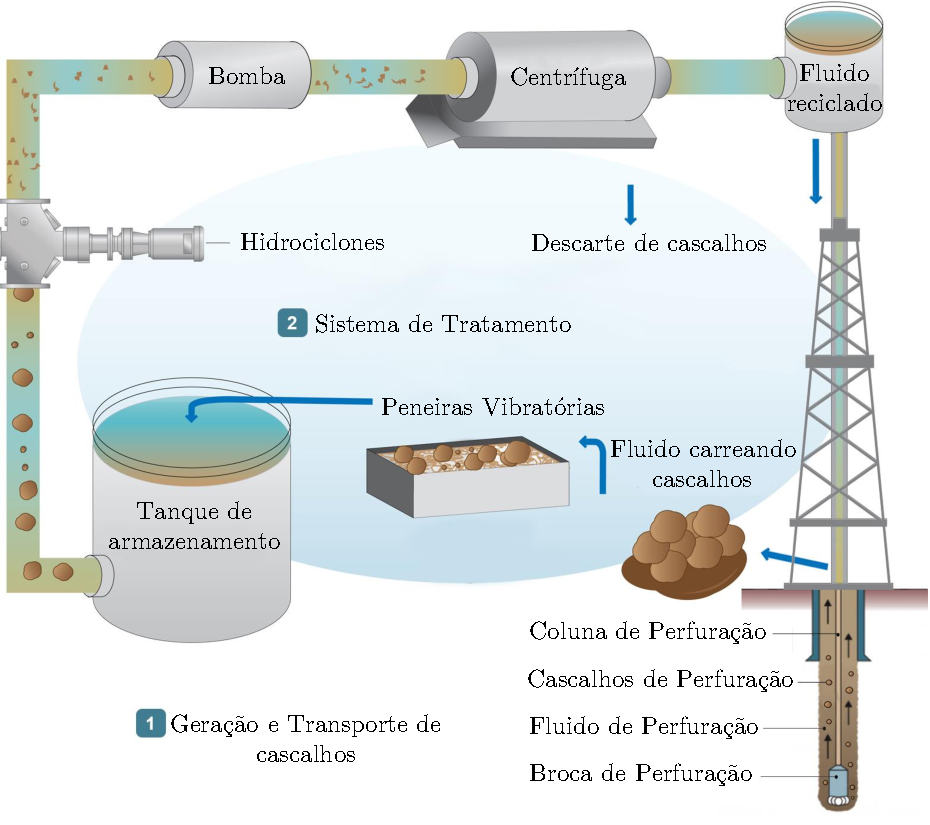
\includegraphics[scale=0.94]{Figuras/esquemaseparacao.pdf}
    \caption{Perfuração de Poços de Petróleo.}
    \legend {Fonte: Adaptado de \citeonline{rbn} e \citeonline{jwce}}
    \label{fig:esquemaseparacao}
\end{figure}

%%%%%%%%%%%%%%%%%%%%%%%%%%%%%%%%%%%%%%%%%%%%%%%%%%%%%%%%%%%%%%%%%%%%%%%%%%%%%%%%%%%%%%%%%%%%%%%%%%%%%%
\subsection{Fluido de Perfuração}

Os fluidos de perfuração são classificados de acordo com o constituinte que apresenta maior proporção em sua mistura, geralmente entre 60\% a 90\% de seu volume físico. Os fluidos são constituídos por uma fase continua que pode ser água, óleo ou gás, a essa fase são adicionados produtos químicos e materiais sólidos que auxiliam a alcançar propriedades específicas necessárias para aumentar a eficiência na operação de perfuração de poços \cite{thomas}.

Os fluidos de perfuração devem possuir características específicas de maneira a garantir uma perfuração eficiente e segura. Dentre as principais funções destacam-se: carrear os cascalhos de perfuração e permitir sua separação na superfície, resfriar a broca e a coluna de perfuração, reduzir o atrito entre a coluna de perfuração e as paredes do poço, manter a estabilidade do poço exercendo pressão hidrostática sobre as formações, para evitar influxo de fluidos da formação para o poço \cite{silva}. No trabalho de \citeonline{pereira}, foi analisada a vazão dos fluidos de perfuração em diferentes profundidades, conforme a Tabela \ref{tab:vazaofluido}.

\begin{table}[!h]
\caption{Vazão do fluido de Perfuração.}
\begin{tabular*}{\textwidth}{@{\extracolsep{\stretch{1}}}*{6}{c}@{}}
   
  \toprule
  Sonda & Fase  & Profundidade do Poço & Vazão do fluido de Perfuração \\
  \midrule
  número&número  & metros &	m³/h \\
  1  &	2 	&2272 &	91\\
 2&	3 	&1619&	98\\
3 &	2 &	610&	82\\
4 &	2&	1282&	91		\\

  \bottomrule   
\end{tabular*}
\label{tab:vazaofluido}
\legend {Fonte: Adaptado de \citeonline{pereira}}
\end{table*}
\end{table}

O fluido de perfuração é a primeira barreira de segurança do poço no processo de perfuração. A densidade do fluido é o parâmetro que regula a pressão hidrostática no poço. Dependo do método de perfuração adotado, a pressão hidrostática gerada pela coluna de fluido no poço, deve ser superior a pressão de poros da formação, afim de evitar influxos, e inferior a pressão de fraturamento da rocha, com o objetivo de evitar a geração de falhamentos. Para que se alcance este valor de equilíbrio existe um estudo geológico prévio que determina a pressão de poros da formação e a pressão de fratura da mesma. A Tabela \ref{tab:densidadefluido}, apresenta as principais características físico-químicas dos fluidos de perfuração utilizados nas atividades de perfuração do Campo de Mexilhão, na Bacia de Santos.

\begin{table}[!h]
\caption{Características físico-químicas dos fluidos de perfuração (Campo de Mexilhão)}
\begin{tabular*}{\textwidth}{@{\extracolsep{\stretch{1}}}*{6}{c}@{}}
   
  \toprule
  & Peso do fluido  & Salinidade & Acidez ou basicidade  \\
   & g/cm³ & mg/L &	pH \\
  \midrule
  Fluido de perfuração SCOL  &	1,44 	&87.000 &	10,0&\\
 Fluido de perfuração catiônico&	1,38 	&103.380&	11,5\\
Fluido de perfuração convencional &	1,07 &	5.000&	9,0\\
Fluido de perfuração STA &	1,32&	85.000&	9,5		\\
BR-MUL HT 1 &	1,50&	310.552&	-	\\
BR-MUL HT 2 &	1,45 &	94.645&	-	\\
  \bottomrule   
\end{tabular*}
\label{tab:densidadefluido}
\legend {Fonte: \citeonline{petrobras}}
\end{table*}
\end{table}


A Reologia desempenha um papel fundamental para otimização e eficiência dos fluidos de perfuração. A Reologia pode ser definida como a ciência que estuda a deformação e o fluxo da matéria. Muitas expressões matemáticas estão propostas na literatura para modelagem  do comportamento reológico de fluidos não newtonianos \cite{reology}.  

Os modelos reológicos descrevem o comportamento da viscosidade do fluido em relação a uma tensão aplicada. Geralmente o modelo de  Bingham e Herschel-Bulkley
representam as características de fluxo de um fluido de perfuração (Figura \ref {fig:bingham}). No modelo de Bingham, é necessário que se alcance a tensão crítica, isto é, tensão mínima para que o fluido comece a
escoar ou entre em movimento. Isto pois, quando o fluido se encontra em repouso, sem sofrer nenhum estado de tensões, a viscosidade aumenta consideravelmente. Ao se aplicar uma tensão mínima de cisalhamento o fluido passa a ter uma viscosidade menor, isto é, a tensão aplicada ao fluido passa a ser proporcional a deformação do mesmo (Fluido newtoniano), mantendo a viscosidade constante a partir desta tensão de cisalhamento mínima. O modelo de Herschel-Bulkley
também necessita de uma tensão de cisalhamento mínima para escoar, porém inicialmente a tensão não é proporcional à deformação do fluido \cite{thomas}. 


\begin{figure}[H]
    \centering
    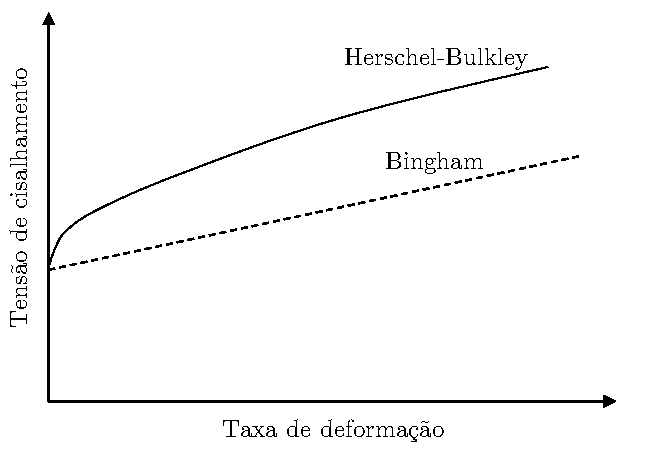
\includegraphics[scale=0.86]{Figuras/bingham.pdf}
    \caption{Modelos reológicos de Bingham e Herschel-Bulkley.}
    \label{fig:bingham}
    \legend{Fonte: Adaptado de \citeonline{reology}}
\end{figure}

A força gel é um parâmetro de natureza reológica que indica o grau de gelificação devido à interação elétrica entre partículas dispersas. A força gel inicial mede a resistência inicial para colocar o fluido em fluxo, ao passo que, a força gel final mede a resistência do fluido para reiniciar o fluxo a partir de um certo tempo em repouso. A diferença entre elas indica o grau de tixotropia do fluido. Os fluidos de perfuração apresentam esta característica tixotrópica, principalmente para manterem os cascalhos suspensos em casos de parada de fluxo, de modo a evitar desmoronamentos no poço \cite{pereira}. 

\citeonline{DYOVANI} comparou a variação na viscosidade aparente de diferentes fluidos de perfuração à base de Goma Xantana. Com base nas curvas de viscosidade foi possível descrever o
comportamento não Newtoniano e pseudoplástico dos fluidos de perfuração. Assim, devido a significante presença da
tensão limite de escoamento, os modelos que
melhor descreveram o comportamento dos fluidos
estudados foram os modelos de Herschel-Bulkley
e Bingham (Figura \ref{fig:fluidoperfura}).

\begin{figure}[H]
    \centering
    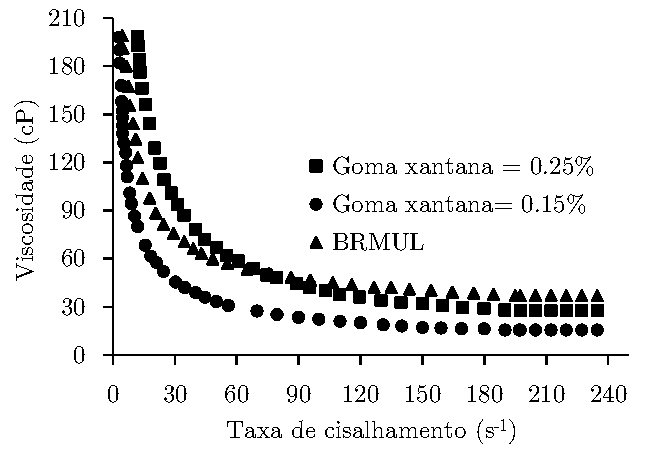
\includegraphics{Figuras/fluidoperfura.pdf}
    \caption{Comportamento reológico de três fluidos de perfuração de poços.}
    \label{fig:fluidoperfura}
    \legend{Fonte: adaptado de \citeonline{DYOVANI}}
\end{figure}

A Figura \ref{fig:fluidoperfura} demonstra que o comportamento da curva de
viscosidade aparente em função da taxa de
cisalhamento, para diferentes concentrações de Goma Xantana, é exponencial (caso fosse constante o fluido seria newtoniano).
Também é constatado o aumento da viscosidade aparente em maiores
concentrações de goma xantana. Em taxas de cisalhamento elevadas existe uma tendência a valores constantes de viscosidade. A
viscosidade aparente do fluido decresceu com o
aumento da taxa de deformação, por outro lado, em baixas taxas de deformação,
o fluido comporta-se semelhante a um corpo sólido, com viscosidade
tendendo a valores extremamente altos, os quais
decaem drasticamente com o aumento da taxa de cisalhamento.


%%%%%%%%%%%%%%%%%%%%%%%%%%%%%%%%%%%%%%%%%%%%%%%%%%%%%%%%%%%%%%%%%%%%%%%%%%%%%%%%%%%%%%%%%%%%%%%%%%%%%%
\subsection{Cascalhos de Perfuração}

Um dos principais resíduos da atividade de perfuração de poços de petróleo são os cascalhos de perfuração. A palavra cascalho de perfuração é uma tradução do inglês “rock cutting”. São fragmentos da formação originados pela ação da broca durante o processo de perfuração de poços e que são carreados para a superfície pelo fluido de perfuração. 
Os cascalhos de perfuração são gerados em todas as fases de perfuração de um poço. Para se estimar a geração de cascalhos de um poço diversas variáveis são levadas em conta. O volume oriundo da perfuração de um poço será dependente da profundidade, características geológicas, tipo de fluido utilizado e diâmetro do poço. Em suma, o volume total de cascalhos deve ser equivalente ao volume nominal do poço (volume do cilindro), ou seja, o volume de cascalho gerados é igual ao volume de poço perfurado por hora \cite{pereira}.

De acordo com \citeonline{fialho}, a partir de dados de perfurações terrestres, no Estado do Espírito Santo são gerados em média 0,13m³ de cascalhos por metro perfurado. \citeonline{schaffel}, determinou que os poços da bacia de campos apresentam aproximadamente entre 0,19m³ e 0,25 m³ de volume de cascalhos produzidos por perfuração. A Tabela \ref{tab:geracaocascalho}, demonstra o volume de cascalhos gerados no Poço P21 (Campo de Mexilhão).

\begin{table}[h]
\caption{Geração de cascalho do Poço P21 (Campo de Mexilhão)}
\begin{tabular*}{\textwidth}{@{\extracolsep{\stretch{1}}}*{6}{c}@{}}
 
  \toprule
    Fase& Profundidade & Diâmetro da broca & Diâmetro do furo & Cascalho Gerado\\
   & metros & polegada &polegada&m³\\
  \midrule
1&410&36”&30”&55\\
2&650&26”&20&82\\
3&2.000&17 ½”&13,375”& 266\\
4&4100&12 ¼” & 9,625”&180\\
5&4721&8 ½”&6,625”& 26\\

  \bottomrule   
\end{tabular*}
\label{tab:geracaocascalho}
\legend {Fonte: \citeonline{petrobras}}
\end{table*}
\end{table}

Os cascalhos de perfuração são resíduos granulares que apresentam características variáveis que vão depender de diversos fatores envolvidos durante a perfuração e, consequentemente, refletidos em suas propriedades físico-químicas. Segundo \citeonline{pereira} dentre os fatores que influenciam as características do cascalho, pode-se destacar: velocidade de perfuração, tipo de broca, diâmetro do poço, tipo de formação perfurada e peso do fluido. A depender desses parâmetros os cascalhos apresentam variabilidade nas características granulométricas (tamanho, forma) e parâmetros químicos, como a densidade. 
A composição química do cascalho é muito variada devido à heterogeneidade das formações atravessadas pela broca, assim como pela presença de contaminantes. Em um estudo com amostras de cascalhos de perfuração em um poço do Espirito Santo, \citeonline{fialho} obteve valores de massa específica equivalente a 2,58 g/cm³ (na fase de perfuração 1) e 2,67 g/cm³ (na fase de perfuração 3). \citeonline{pereira} encontrou valores próximos, com variação de 2,5 g/cm³ até 2,8g/cm³, tendo um valor médio de massa específica de 2,6 g/cm³. A Tabela \ref{tab:composicaocascalho} revela a proporção mineralógica dos cascalhos registrados em poços de perfuração por diversos autores. 


\begin{table}[!h]
\caption{Composição dos cascalhos de Perfuração.}
\begin{tabular*}{\textwidth}{@{\extracolsep{\stretch{1}}}*{6}{c}@{}}
 \toprule
   &ABBE et al (2009)& Medeiros (2010) & Leonard e Stegeman (2010)\\
  \midrule
SiO2&37,60&36,5&60,40 \\
Al2O3&13,54&11,5&10,40\\
Fe2O3&6,34&4,5&4,90\\
BaO&11,39&-&- \\
CaO&2,78&35,3&2,50\\

  \bottomrule   
\end{tabular*}
\label{tab:composicaocascalho}
\legend {Fonte: \citeonline{fialho}}
\end{table*}
\end{table}

Em geral, os cascalhos apresentam características físicas variadas a depender dos fatores citados anteriormente. Esses parâmetros físicos descrevem o tamanho do particulado, bem como fatores de forma da partícula (Esfericidade e razão de aspecto). A determinação da distribuição de tamanho e da forma de amostras de cascalhos de perfuração em diferentes profundidades (Grupo), realizadas por meio da técnica de análise dinâmica de imagens está apresentada na Tabela \ref{tab:granulometriacascalho}.


\begin{table}[!h]
\caption{Tamanho e forma (esfericidade) de amostras de cascalhos de Perfuração.}
\begin{tabular*}{\textwidth}{@{\extracolsep{\stretch{1}}}*{6}{c}@{}}
 \toprule
   Grupo &D[10]& D[50]& D[90]& D[médio]& Esfericidade \\
  \midrule
A - 2.376 &286,6 & 531,8 &1010,6& 588,2 & 0,787\\
B - 5.142 &345,5 &763,4 &1430,5 &828,6 & 0,765\\
C - 2.433 &169,3 &325,0 &682,4 &375,5  &0,783 \\
D - 2.529 &268,3 &468,3 &913,4 &753,4  &0,758 \\
E - 2.700 &273,8 &512,7 &1091,8 &599,1 & 0,792 \\
F - 3.201 &311,2 &562,7 &1257,0 &678,5  &0,777 \\
G - 3.312 &353,8 &661,8 &1342,3 &759,0 & 0,778 \\
H - 3.543 &315,5 &665,0 &1171,2 &713,2 & 0,776 \\
I - 3.564 &167,0 &321,1 &597,2 &352,4  &0,789 \\
J - 4.758 &339,7 &698,8 &1434,5 &805,5  &0,745 \\
K - 4.920 &335,1 &654,4 &1292,7 &732,9  &0,765 \\
L - 5.400 &521,3 &1107,47& 2105,5 &1222,5&  0,785\\
M - 4.824 &392,1 &719,1& 1554,0 &865,0 & 0,750 \\
N - 4.842 &356,0 &642,8& 1362,7 &757,6&  0,755\\

  \bottomrule   
\end{tabular*}
\label{tab:granulometriacascalho}
\subcaption{D[X]= diâmetro/ área abaixo do qual estão X\% das partículas (\mu  m).

D[médio] = diâmetro / X área médio (\mu  m).

Esfericidade (SPHT) = relação entre a área da partícula e seu perímetro.}
\legend {Fonte: \citeonline{bortotti}}
\end{table*}
\end{table}

No estudo de \citeonline{bortotti}, o tamanho dos cascalhos variou de d[10] 169,3 µm
(areia fina) até [d90] 2105,5 µm (cascalho muito fino), tendo diâmetro médio de
700,9 µm (areia grossa). Em relação ao fator de forma dos cascalhos,  75\%  das amostras apresentaram
esfericidade acima de 0,745. O grupo J foi o menos esférico,
tendo a esfericidade (SHPT) variando aproximadamente entre 0,511 D[10], 0,745 D[médio] e 0,888 D[90].
%%%%%%%%%%%%%%%%%%%%%%%%%%%%%%%%%%%%%%%%%%%%%%%%%%%%%%%%%%%%%%%%%%%%%%%%%%%%%%%%%%%%%%%%%%%%%%%%%%%%%%

\section{Erosão por partículas sólidas}
\label{cap:Erosão por partículas sólidas}


Erosão é a perda de material que constitui um equipamento ou tubulação de forma progressiva causada pelo impacto repetitivo de partículas sólidas ou liquidas contra a superfície de um corpo sólido. Isto ocorre devido ao arraste destas partículas por algum fluido até a superfície sólida do material alvo \cite{hutchings}.

No desgaste erosivo por partículas sólidas, várias forças de diferentes origens podem atuar sobre uma partícula em contato com uma superfície sólida (Figura \ref{fig:erosaoforca}). Partículas adjacentes podem exercer forças de contato e sob algumas condições, a gravidade pode exercer alguma influência. No entanto, a força dominante sobre uma partícula erosiva, que é a principal responsável por desacelerá-la da sua velocidade de impacto inicial, é a força de contato exercida pela superfície do material no momento de choque.

%%%%%%%%%%%%%%%%%%%%%%%%%%%%%FIGURA%%%%%%%%%%%%%%%%%%%%%%%%%%%%%%%%%%%%%%%%%%%%%%%%%%%%%%%%%%%%%%%
\begin{figure}[!h]
    \centering
    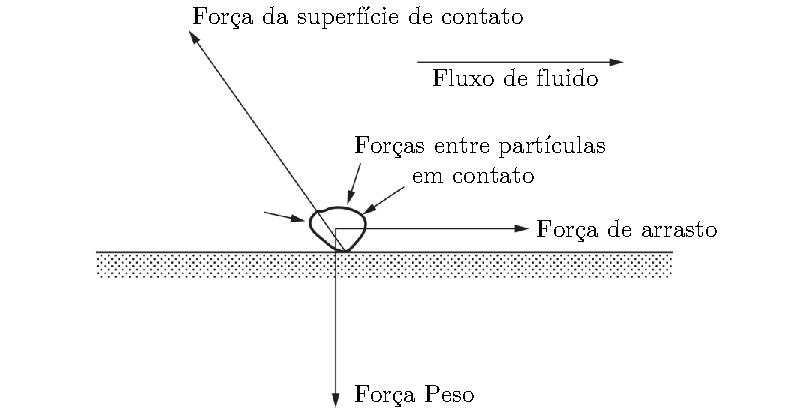
\includegraphics{Figuras/erosaoforca.pdf}
    \caption{Diagrama com as
forças sobre
partícula em contato com uma superfície sólida
}
\label{fig:erosaoforca}
\legend {Fonte: Adaptado de \citeonline{hutchings}}
\end{figure}
%%%%%%%%%%%%%%%%%%%%%%%%%%%%%FIGURA%%%%%%%%%%%%%%%%%%%%%%%%%%%%%%%%%%%%%%%%%%%%%%%%%%%%%%%%%%%%%%%

A erosão causada por partículas sólidas é um dos principais mecanismos de desgaste responsáveis por falhas em equipamentos presentes na indústria petrolífera. A produção de cascalhos durante a perfuração de poços pode causar danos erosivos consideráveis em tubulações, conexões, máquinas e equipamentos de separação sólido-líquido conectados a essas tubulações (Figura \ref{fig:erosaoperf}). O dano é pronunciado em regiões onde há uma mudança abrupta na direção do fluxo como curvas, válvulas e cotovelos que são partes integrantes da tubulação dos sistemas hidráulicos \cite {kumar}. 

\begin{figure}[H]
    \centering
    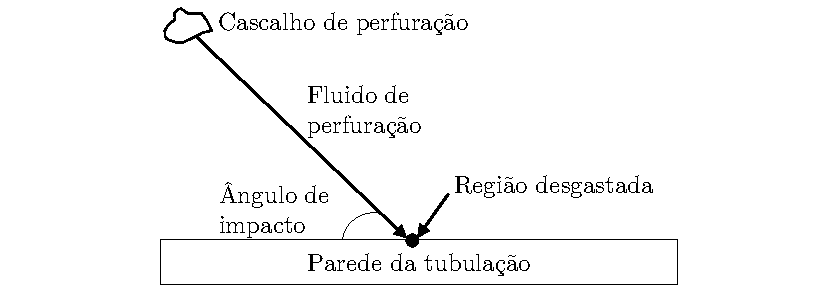
\includegraphics{Figuras/desgasteerosivoPerf.pdf}
    \caption{Desgate erosivo em linhas hidráulicas de perfuração de poços petrolíferos.}
\label{fig:erosaoperf}
\legend {Fonte: Adaptado de \citeonline{ANUR}.}
\end{figure}

O fenômeno da erosão é altamente complexo e uma ampla gama de parâmetros podem afetar a taxa de desgaste erosivo num determinado material. Vários pesquisadores mediram e quantificaram o efeito de diferentes parâmetros na erosão por partículas sólidas a qual pode ser classificada em quatro grupos de variáveis: as características da partícula erosiva, as características de impacto, as características de fluido e escoamento e as propriedades do material alvo. Estes grupos são apresentados em um diagrama típico de causa e efeito (Figura \ref{fig:erosaopeixe}) e são discutidos nos próximos parágrafos.

%%%%%%%%%%%%%%%%%%%%%%%%%%%%%FIGURA%%%%%%%%%%%%%%%%%%%%%%%%%%%%%%%%%%%%%%%%%%%%%%%%%%%%%%%%%%%%%%%%
\begin{figure}[H]
    \centering
    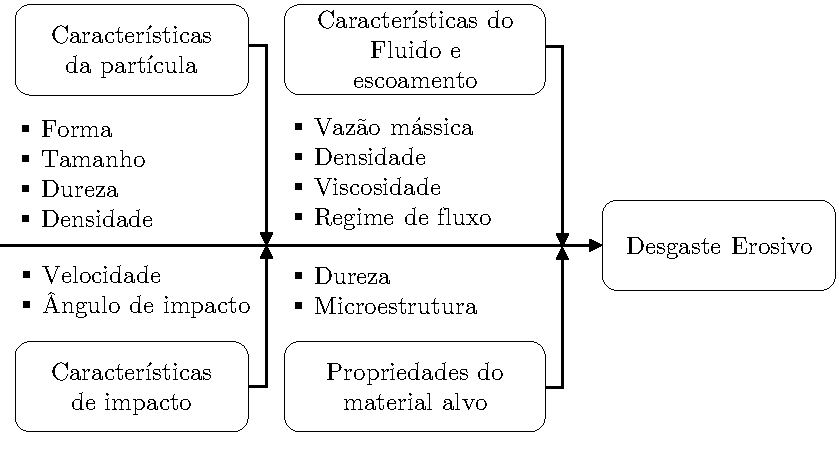
\includegraphics{Figuras/erosaopexie.pdf}
    \caption{Atributos que influenciam no desgaste erosivo.}
    \legend {Fonte: Adaptado de \citeonline{ANUR}.}
    \label{fig:erosaopeixe}
\end{figure}

%%%%%%%%%%%%%%%%%%%%%%%%%%%%%FIGURA%%%%%%%%%%%%%%%%%%%%%%%%%%%%%%%%%%%%%%%%%%%%%%%%%%%%%%%%%%%%%%%

A influência das propriedades e características das partículas foram estudadas em diversos trabalhos na literatura e são propriedades relevantes no desgaste erosivo. Em geral, partículas maiores resultam no aumento da taxa de erosão. Além da maior energia de impacto, o tamanho da superfície de contato tende a ser mais abrangente, levando a um maior desgaste no material \cite{zum} \cite{lieb}. Por outro lado, a alteração no tamanho das partículas pode influenciar nas direções de fluxo, o que resulta na mudança das regiões de colisão no material \cite {clark}. 

O estudo de \citeonline{hutchings} determinou que para calcular a taxa de erosão foi preciso verificar a forma das partículas erodentes, para isto propôs uma metodologia para a medição da forma das partículas utilizando um parâmetro (F), denominado fator de esfericidade. Este cálculo consiste na relação entre a área de projeção bidimensional das partículas e a área de um círculo com perímetro igual ao da projeção. No mesmo estudo, realizou experimentos envolvendo partículas esféricas e angulares. O impacto causado por partículas esféricas resultam em menor deformação localizada, ou seja, a taxa de erosão foi maior nos ensaios em que as partículas eram circulares \cite{walker}. 

Uma variável determinante na taxa erosiva é relação entre a dureza da partícula e a dureza do material alvo \cite{hutchings}. Em geral, partículas com menor dureza que o material causam menor desgaste comparado a partículas mais duras. \citeonline{divakar} alteraram a dureza do aço AISI 316 por laminação a frio e mostrou que um aumento na dureza diminui a erosão total em um testador de erosão a jato. Geralmente, com um aumento na dureza da partícula erodente, há um acréscimo na erosão total até certo limite, acima deste limite o aumento da dureza da partícula tem pouco efeito. \citeonline{levy} realizou testes de erosão em aço carbono AISI 1020 com dureza de 150 kgf/mm² utilizando partículas com diferentes níveis de dureza, ou seja, calcita, apatita, areia, alumina e carboneto de silício, no qual mostrou que acima de uma dureza de partícula de 700 kgf/mm², a taxa de erosão permaneceu constante. 

Em um fluxo multifásico líquido-sólido, a velocidade de impacto de uma partícula é uma função da velocidade de fluxo do fluido e a inércia da partícula em resistir à força de arrasto exercida pelo líquido. Deste modo, uma partícula de alta densidade apresenta uma velocidade de impacto maior do que uma de baixa densidade. Da mesma forma, a eficiência de colisão para partículas de alta densidade é maior do que as de baixa densidade em condições de teste idênticas. Portando, o efeito da colisão em maiores velocidades é o aumento da energia cinética de impacto, que juntamente com maior eficiência de colisão, resulta em maiores taxas de desgaste erosivo para partículas mais densas \cite {clark2}.
Uma das variáveis envolvidas no impacto é a velocidade da partícula no momento da colisão com o material erodido. Diversos pesquisadores constataram experimentalmente que a velocidade da partícula no momento do impacto com o material influencia diretamente na taxa de erosão. Isto está relacionado ao efeito da energia cinética das partículas erosivas \cite {lind}, \cite {trus}, \cite {finnie2}. No entanto, a partícula erodente tem que atingir uma velocidade crítica para induzir a deformação plástica na superfície do material alvo. Em velocidades de fluxo mais baixas, a maioria das partículas têm velocidades abaixo de um valor limite que resultam em deformação elástica, deste modo, é observado menor desgaste erosivo. Por outro lado, quando as partículas abrasivas atingem velocidade superior ao valor crítico, o impacto contínuo das partículas desenvolve plaquetas plasticamente deformadas que são removidas após impactos adicionais, o que significa maior desgaste erosivo \cite {yabuki}.

O ângulo de impacto, que é o ângulo entre a trajetória da partícula e a superfície do alvo, também pode afetar o desgaste erosivo no material. A variação da taxa de erosão em diferentes ângulos de impacto depende da ductilidade do material alvo. Em materiais dúcteis, a erosão máxima ocorre em ângulos de impacto entre 40° e 50°, enquanto para materiais frágeis a taxa de erosão máxima ocorre próximo de 90° \cite{albu}.

Diversos estudos, revelaram que quanto maior a concentração de partículas presentes no fluxo, maior a taxa de erosão devido ao número crescente de partículas que atingem a superfície da parede do alvo \cite{gandhi}. Ou seja, a taxa de erosão aumenta linearmente com a carga de partículas sólidas. Porém, existem situações em que o aumento da concentração de partículas erosivas pode gerar o aumento da quantidade de choques entre as partículas e a consequente diminuição de energia cinética de impacto, neste caso não ocorre a linearidade entre a concentração de partículas e o aumento de desgaste erosivo.  Outro caso é o fenômeno de incubação, em que ocorre a deposição de partículas na superfície do material erodido em função do aumento de partículas no escoamento e das condições de viscosidade do fluido \cite{tsai}. 

A viscosidade do fluido possui influência direta nas trajetórias das partículas, nas velocidades de impacto e nos ângulos de impacto, sendo um fator que determina a eficiência de colisão erosiva, isto é, a relação entre a quantidade total de partículas e a quantidade de partículas que efetivamente impactam contra a superfície do material alvo. Fluidos viscosos aumentam a flutuabilidade das partículas sólidas mantendo-as suspensas durante o fluxo. No caso de fluxos com líquidos menos viscosos, as partículas sólidas tendem a se depositar na superfície do material erodido \cite {yabuki}. Ou seja, significa que geralmente a perda de material é reduzida com a diminuição da viscosidade do fluido. No entanto, o efeito de viscosidade depende da velocidade do líquido. Em baixas velocidades superficiais (18, 27, 35 m/s), a perda de metal aumentou com o aumento da viscosidade do líquido, enquanto diminuiu em altas velocidade (45 m/s) \cite {yabuki}. \citeonline{kowsari} propuseram que, em uma velocidade muito alta (110 m/s), um aumento na viscosidade causa uma diminuição na erosão devido a dois efeitos viscosos. Primeiro, o aumento da viscosidade altera a zona de estagnação e, assim, reduz a energia de impacto das partículas e a capacidade erosiva. Em segundo lugar, uma maior viscosidade de fluido aumenta número de equilíbrio de momento, conforme, causando uma maior tendência das partículas seguirem as linhas de corrente. Isso, por sua vez, diminue o ângulo de impacto local na parte inferior do canal e reduz a taxa de erosão.

O impacto das partículas contra o material erodido é mais frequente em condições de fluxo turbulento. Assim, em fluxos laminares a taxa de desgaste é relativamente reduzida, pois neste regime de escoamento as partículas se movem paralelamente à superfície do material, diminuindo a possibilidade de geração de condições em que ocorrem impactos diretos em sua superfície.

A microestrutura do aço desempenha um papel importante na taxa de erosão. Dados de taxa de erosão normalizados indicam que a perlita é mais eficaz na resistência à erosão do que a ferrita, devido à sua estrutura lamelar, que é capaz de absorver a energia das partículas impactantes \cite{yabuki}.



%%%%%%%%%%%%%%%%%%%%%%%%%%%%%%%%%%%%%%%%%%%%%%%%%%%%%%%%%%%%%%%%%%%%%%%%%%%%%%%%%%%%%%%%%%%%%%%%%%%%%%%%%%


\section{Simulação Fluidodinâmica computacional (CFD)}
\label{Simulação Fluidodinâmica computacional (CFD)}

Podemos geralmente definir fluidodinâmica computacional (CFD) como simulações feitas a partir de computador, através de resolução de equações, com objetivo de analisar sistemas complexos que incluem transferência de calor, fluxos de fluidos e reações químicas \cite{versteeg}. O modelo de simulação objetiva representar em um ambiente computacional as características que o sistema apresentaria em condições semelhantes de contorno. 


Os códigos para simulação fluidodinâmica computacional são voltados para algoritmos numéricos configurados em interface gráfica de usuário, que facilitam a inserção dos parâmetros de entrada, o processo de solução e a visualização dos resultados da simulação. As principais etapas de um pacote CFD são definidas como: identificação do problema, pré-processamento, solução e pós-processamento (Figura \ref{fig:etapascfd}). O métodos utilizado em CFD para resolução das equações é método dos volumes finitos (MVF), que se baseia na aplicação de integrais para cálculos de conservação de energia, massa e momentum, podendo prever numericamente o comportamento de fluxos multifásicos e turbulentos relativamente complexos.  As próximas seções apresentam um breve resumo das etapas envolvidas em uma simulação computacional CFD.

%%%%%%%%%%%%%%%%%%%%%%%%%%%%%FIGURA%%%%%%%%%%%%%%%%%%%%%%%%%%%%%%%%%%%%%%%%%%%%%%%%%%%%%%%%%%%%%%%
\begin{figure}[H]
    \centering
    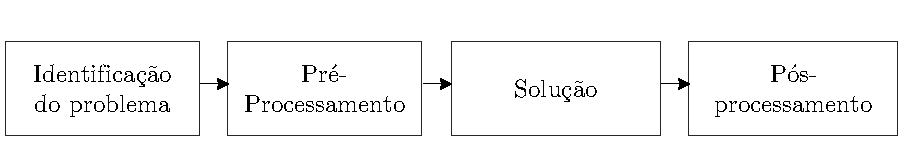
\includegraphics{Figuras/cfd.pdf}
    \caption{Etapas da simulação fluidodinâmica computacional.}
    \legend {Fonte: \citeonline{versteeg}}
    \label{fig:etapascfd}
\end{figure}
%%%%%%%%%%%%%%%%%%%%%%%%%%%%%FIGURA%%%%%%%%%%%%%%%%%%%%%%%%%%%%%%%%%%%%%%%%%%%%%%%%%%%%%%%%%%%%%%%%%

É necessário definir inicialmente qual o problema em questão que necessita ser modelado. Isso pode resultar em simplificações na criação da geometria, de forma a evitar gasto de tempo e capacidade computacional em regiões que não são de interesse no estudo fluidodinâmico. Na fase de pré-processamento é realizada a elaboração da geometria através de desenho assistido por computador (CAD). A geometria deve caracterizar toda a região onde ocorre o escoamento \cite{petrila}.

O método de volumes finitos é utilizado em simulações CFD, este consiste na divisão do espaço físico em blocos separados conhecido como malha computacional. Esta é a fase da discretização do modelo, onde a estrutura geométrica é dividida em volumes de controle, os quais representam a porção onde são empregados métodos numéricos na resolução das equações. Após definido os volumes de controle, são configurados os parâmetros físicos utilizados pelo solver para o cálculo do problema físico estudado \cite{anderson}.

A Solução é a etapa de processamento onde ocorre a resolução das equações no espaço e no tempo, ou seja, as equações de conservação de massa, energia e quantidade de movimento. Todas as grandezas físicas são calculadas em um mesmo passo do tempo (iteração), de forma que são feitas até atingir a convergência ou número de iterações estabelecidas \cite{batchelor}.

Na etapa de pós-processamento, os resultados são apresentados e analisados. Deste modo, é possível visualizar os valores e apresentar os resultados de interesse de forma iterativa, obtendo valores de grandezas físicas em qualquer parte do volume de controle do material estudado \cite{versteeg}.


\subsection{Modelagem Matemática e Computacional dos Escoamentos}

Na perfuração de poços de petróleo, ao fragmentarem e serem carregados pelo fluido de perfuração, os cascalhos juntamente com o fluido formam um sistema multifásico de escoamento. A modelagem computacional apresenta as equações governantes do problema, as condições de contorno, e as equações constitutivas necessárias que complementam a modelagem.

Quando o escoamento é laminar, é facilmente modelado e simulado pelo programa. Porém, as simulações de escoamentos turbulentos apresentam maior custo computacional e complexidade envolvida. O escoamento turbulento é caracterizado como uma condição irregular de escoamento, ou seja, são instáveis, com múltiplas escalas, rotacionais, tridimensionais, com alta difusibilidade e de forma contínua \cite{turb}.
Dado a importância da caracterização de escoamento turbulento, foram desenvolvidos métodos de solução computacional para representação desse fenômeno físico. O escoamento turbulento pode ser dimensionado por três diferentes técnicas: Simulação Numérica Direta (DNS) Simulações de Grandes Escalas (LES) ou através das equações de Navier-Stokes com médias de Reynolds (RANS) \cite{turb}.

A modelagem Navier-Stokes com médias de Reynolds (RANS) é a mais utilizadas para modelagem de escoamento turbulento. Este modelo de cálculo de turbulência resulta em menor esforço computacional comparado aos demais \cite{versteeg}. As equações são caracterizadas pela decomposição da velocidade em termos de um valor médio e de flutuação. O Tensor específico de Reynolds ocorre como resultado dos processos de média de Reynolds aplicados às equações de conservação de massa e de quantidade de movimento. Para determinação do tensor específico de Reynolds se faz necessário o uso de modelos de turbulência, dentre os modelos existentes destacam-se:  k-ω; k-ω SST; k-Є Standard; k-Є RNG; k-Є Realizable \cite{versteeg}. O modelo k-Є Standard usa duas equações de transporte,  é o modelo mais utilizado atualmente, pois possui um baixo custo de processamento computacional e descreve de forma satisfatória escoamentos turbulentos.

O escoamento multifásico é caracterizado pela presença de mais de uma fase num determinado sistema, portanto, na perfuração de poços de petróleo, ao fragmentarem e serem carreados pelo fluido de perfuração, os cascalhos juntamente com o fluido formam um sistema multifásico de escoamento. Assim, para um fluxo líquido-sólido, a fase contínua é dominante durante o escoamento. Já a fase dispersa é a fase carreada pelo contínuo. Deste modo, num fluxo envolvendo fluido de perfuração e cascalhos, o fluido é a fase contínua e os cascalhos a fase dispersa.  As técnicas de modelagem de fluxo multifásico são divididas em dois grupos: Euleriano-Euleriano e Euleriano-Lagrangeano.

No Modelo Euleriano-Euleriano, as fases envolvidas são tratadas matematicamente como fases continuas interpenetrantes \cite{ansys}. Neste modelo o local onde se encontra uma fase não pode ser ocupado pela outra fase. Já no modelo Euleriano-Langrageano (Modelo de fase discreta), uma das fases é tratada como continua (Euleriano), resolvendo as equações de Navier-Stokes. A outra fase é considerada discreta (Langrageana), cujas equações de movimento são baseadas na segunda Lei de Newton para o deslocamento de partículas. Este modelo é utilizado no presente trabalho e será descrito a seguir.

A forma de modelagem Euleriana-Lagrangeana no Ansys é denominada DPM (Discrete Phase Model) ou Modelagem da Fase Discreta. Para utilização deste modelo é necessário que a fase discreta tenha proporção volumétrica menor que 10\% em relação a fase contínua, de modo que as partículas no sistema não influenciem no fluxo da fase contínua. Assim, o equacionamento da trajetória da partícula lagrangeana é calculado separadamente da fase contínua. Para se prever a trajetória e direção de movimento das partículas (Velocidade e posição), faz-se a integral do balanço de forças na partícula em relação a sua inércia (com base na segunda lei de newton) de acordo com a equação \ref{eqn:euleriano} (unidades em SI), utilizando um referencial Langrageano. Essas integrais são resolvidas gradualmente ao longo de cada passo de tempo das simulações.

\begin{equation}
\frac{\partial uv}{\partial{}t}=Fd (v-uv)+ \frac{gx(\rho\rho -\rho )} {\rho\rho}+Fi
\end{equation}
\begin{equation}
FD=\frac{18u}{pp {dp}^2} \frac{CdRe}{24}
\label{eqn:euleriano}
\end{equation}

Onde:

 Fi= é um termo de aceleração adicional (força por massa de uma unidade de partícula;
 
 Fd (u-uv)= é a força de arrasto por massa de uma unidade de partícula;
 
 v= é a velocidade da fase contínua;
 
 uv= é a velocidade da partícula;
 
 u= viscosidade molar do fluido;
 
 p= é a densidade do fluido;
 
 pp= é a densidade da partícula;
 
 dp= é o diâmetro da partícula.


%%%%%%%%%%%%%%%%%%%%%%%%%%%%%%%%%%%%%%%%%%%%%%%%%%%%%%%%%%%%%%%%%%%%%%%%%%%%%%%%%%%%%%%%%%%%%%%%%%%%%%

\subsection{Simulação numérica para previsão do desgaste erosivo}

A previsão de erosão é sempre uma tarefa difícil na indústria de petróleo e gás devido ao desafio de entender, sob circunstâncias complexas de comportamento de fluxo, a distribuição das partículas sólidas ao longo do escoamento e os locais propensos ao impacto nos diversos equipamentos envolvidos nas etapas de exploração e produção. Outrossim, diversos parâmetros podem influenciar este tipo de desgaste em diferentes magnitudes, como demonstrado no Capítulo \ref{cap:Erosão por partículas sólidas}.

A complexidade da previsão de erosão aumenta significativamente em fluxos multifásicos em que gases, líquidos e sólidos podem estar presentes simultaneamente no escoamento.  Este regime de fluxo é dependente do tamanho da tubulação, ângulos de inclinação e propriedades do fluido que afetam significativamente as regiões e velocidade de impacto das partículas sólidas no material.

Nos últimos anos, a simulação fluidodinâmica computacional emergiu como uma ferramenta preferida para a previsão de erosão. Isto se deve ao fato de ser capaz de reproduzir condições de fluxos multifásicos e turbulentos e permitir o rastreamento da trajetória de partículas nestes sistemas \cite{yuhan} \cite {Parsi}. Deste modo, é possível obter uma compreensão dos efeitos do fenômeno físico erosivo através da identificação dos locais mais propenso ao impacto das partículas, prever a taxa máxima de erosão e o efeito de diferentes parâmetros no desgaste erosivo. A abordagem CFD também surge como uma alternativa de estudo em casos que a criação de uma análise experimental é difícil. A Figura \ref{fig:cfderosao}, demonstra uma simulação de fluxo de fluido ao longo de uma turbulação de geometria curva. Deste modo, é possível verificar que a simulação CFD determinou os locais de impacto das partículas sólidas no material e foi capaz de prever as regiões com maiores taxas de desgaste erosivo, representadas pelo gradiente de cores. Em contrapartida, para um estudo experimental as regiões de maiores desgastes são justamente os locais onde ocorre a falha do material.

%%%%%%%%%%%%%%%%%%%%%%%%%%%%%FIGURA%%%%%%%%%%%%%%%%%%%%%%%%%%%%%%%%%%%%%%%%%%%%%%%%%%%%%%%%%%%%%%%
\begin{figure}[H]
    \centering
    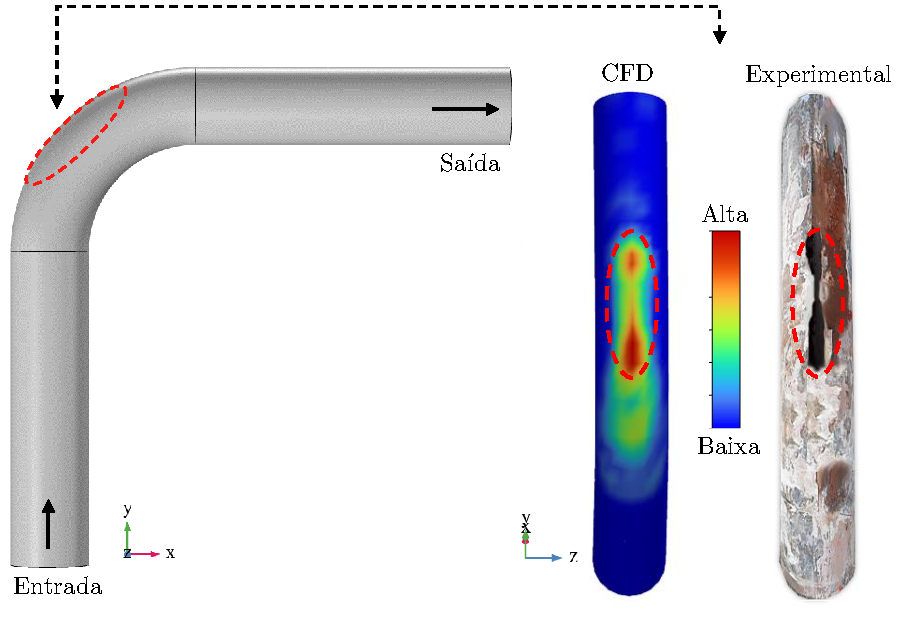
\includegraphics{Figuras/cfderosao.pdf}
    \caption{Simulação fluidodinâmica computacional para a previsão do desgaste erosivo.}
    \label{fig:cfderosao}
    \legend {Fonte: o autor.}
\end{figure}
%%%%%%%%%%%%%%%%%%%%%%%%%%%%%FIGURA%%%%%%%%%%%%%%%%%%%%%%%%%%%%%%%%%%%%%%%%%%%%%%%%%%%%%%%%%%%%%%%

Diversos estudos para o desenvolvimento de equações e modelos analíticos para avaliar a erosão em condições de escoamento monofásico e multifásico foram publicados \cite {oka} \cite {dnv} \cite {finnie} \cite{maclaury}. Porém cada modelo foi desenvolvido sob condições especificas de experimentos, o que influencia diretamente nas variáveis consideradas no cálculo erosivo, haja vista que existem muitos fatores que podem afetar a taxa de erosão. Portanto, existe pouco consenso na literatura sobre a melhor forma de prever quantitativamente a taxa erosiva. Deste modo, a depender do tipo de material avaliado e as condições de escoamento existentes, é possível definir um modelo de erosão específico que atende melhor a previsão do desgaste erosivo com base em validação com dados experimentais.

No estudo de \citeonline{liuuh}, foram feitas simulações CFD para previsão de erosão em curvas de aço carbono com raio de curvatura de 90°, em escoamento turbulento líquido-sólido. Após comparação com vários outros quatro modelos encontrados na literatura, resultados experimentais e validações publicadas, o modelo de \citeonline{oka} se provou o mais adequado para as condições de validação entre modelo numérico e experimental para erosão em curvas de 90° de raio curto e sob as condições de escoamento estudadas. As equações que representam o modelo de Oka, se encontram dispostas a seguir: 

\begin{equation}
    E(\alpha) = g(\alpha)E90
    \label{equationoka}
\end{equation}
\begin{equation}
E90=K(aHv)^{k1b}  \left ( \frac{v}{v'} \right )^{k2} \left ( \frac{d}{d'} \right )^{k3} 
\end{equation}
\begin{equation}
g(\alpha)= (sin   \alpha)^{_{n1}}(1+Hv(1-sin  \alpha))^{^{n2}}
\end{equation}
\begin{equation}
n1=s1(Hv)^{q1}
\end{equation}
\begin{equation}
n2=s2(Hv)^{^{q2}} 
\end{equation}
\begin{equation}
k2=2.3(Hv)^{0.038} 
\end{equation}

Onde: 

E ($\alpha$) = é a taxa de erosão em determinado ângulo.

E90= é a taxa de erosão em ângulo de 90 graus (taxa de erosão na direção normal); 

g ($\alpha$) = função do ângulo de impacto (graus);

k, k1 e k3= são constantes determinadas pelas propriedades das partículas;

k2= é uma função da dureza do material e de propriedades da partícula;

V= velocidade de impacto da partícula (m/s);

D= diâmetro da partícula ($\mu$m);

V'= velocidade de referência do experimento de Oka (m/s);

D'= diâmetro da partícula de referência do experimento de Oka ($\mu$m);

Hv= é o número de dureza de Vickers do material alvo (em GPa).


%%%%%%%%%%%%%%%%%%%%%%%%%%%%%%%%%%%%%%%%%%%%%%%%%%%%%%%%%%%%%%%%%%%%%%%%%%%%%%%%%%%%%%%%%%%%%%%%%%%%%%%%%%%%%%%%%%%
\section{Análise de risco}

O risco pode ser entendido como uma função de incertezas envolvidas em um projeto, que para a indústria de Óleo e Gás podem ser geológicas, econômicas e tecnológicas, cujas análises possam ser integradas. O entendimento de risco de um projeto contribui para a tomada de decisão durante o processo de perfuração de poços. Sob a perspectiva de falha dos componentes, a quantificação de risco representa a otimização na determinação da manutenção preventiva, troca dos equipamentos se seleção adequada de equipamentos.

A análise de risco de um projeto de Perfuração de poço petrolífero requer informações detalhadas a respeito das propriedades e características relativas as rochas e fluidos de perfuração, sendo necessário o entendimento dos parâmetros fluidodinâmicos e petrofísicos integrados, que podem ser caracterizados através da simulação numérica computacional \cite{loschiavo}. Embora seja amplo, o conceito de incerteza utilizado neste trabalho está relacionado à falta de conhecimento dos valores precisos dos atributos que influenciam no desgaste erosivo, ou seja, a incerteza dos atributos causa incerteza na previsão do desgaste erosivo de um projeto de perfuração de poços. Deste modo, a combinação das variáveis aleatórias que influenciam no desgaste erosivo, em diversos cenários, resultam na quantificação de risco para tomada de decisão.

A etapa preliminar da análise de risco consiste na seleção e caracterização dos atributos geológicos e físicos a serem utilizados na análise de incertezas. A incerteza do atributo deve ser expressa através de sua distribuição de probabilidade para o processo de análise de risco. Na prática, os dados disponíveis geralmente não são suficientes para o correto conhecimento das variáveis analisadas. Em muitos casos são obtidos apenas os valores mínimos, prováveis e máximos dos atributos, através de dados amostrais ou estimados por especialistas (Engenheiros, geólologos, geofísicos e petrofísicos) ou a partir do conhecimento que se tem de poços vizinhos. Os atributos também podem ser definidos pela divisão ou multiplicação do valor mais provável \cite{steagall}.

A quantidade de variáveis de entrada do modelo determina o esforço e tempo computacional para simulações de cenários probabilísticos. Portanto, uma etapa essencial para a análise de risco é o estudo de sensibilidade, que consiste na definição dos atributos críticos, ou seja, as variáveis que mais exercem impacto na resposta da simulação numérica (desgaste erosivo). Esse processo tem por finalidade a redução do número de variáveis utilizadas no estudo. Dado que, a aplicação de todos os atributos incertos pode ser inviável computacionalmente, pois o número de simulações cresce com a quantidade de variáveis, e de mesma forma desnecessária, pois algumas variáveis podem causar impactos mínimos na quantificação de risco \cite{santoss2}. A análise de sensibilidade é um método que consiste em variar os atributos em um nível inferior e superior e observar o impacto desta variação na Função-objetivo, o que permite estimar quais fatores apresentam maior influência na resposta. O planejamento de Plackett-Burman pode ser utilizado para a triagem dos fatores, ou seja, determinar o impacto das variáveis sobre a função-objetivo, uma vez que são capazes de obter informações sobre os efeitos  principais e as interações entre as variáveis simultaneamente \cite{plackett}. Deste modo, utilizando o planejamento estatístico para a realização do estudo de sensibilidade, pode-se determinar os fatores críticos para aplicação dos métodos de combinação dos atributos para análise de risco.


\subsection{Método da Àrvore de Derivação}

A análise de risco baseada na Metodologia da Árvore de Derivação tem como base a simulação numérica de vários cenários possíveis, através da combinação de atributos. Os atributos são discretizados em níveis de incerteza, aos quais estão associadas determinadas probabilidades de ocorrência de acordo com sua distribuição de probabilidade \cite{madeira}. A Figura \ref{fig:arvorederivacao} demonstra uma árvore de derivação constituída por 2 atributos, ambos com três níveis de ocorrência com probabilidade associada.

\begin{figure}[H]
    \centering
    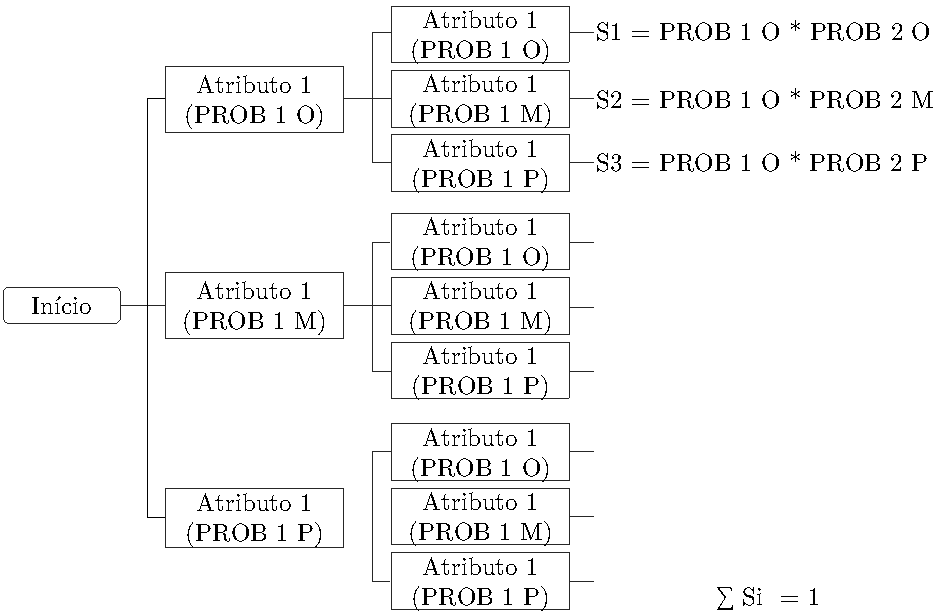
\includegraphics[scale=1]{Figuras/derivacao.pdf}
    \caption{Exemplo de árvore de derivação - 2 atributos com 3 níveis.}
    \legend {Fonte: Adaptado de \citeonline{madeira}}
    \label{fig:arvorederivacao}
\end{figure}

Todos os cenários representados na árvore são submetidos à simulação fluidodinâmica computacional.
A probabilidade de ocorrência de cada cenário de simulação fluidodinâmica corresponde ao produto das probabilidades de ocorrência dos níveis dos atributos presentes no modelo. Cabe citar que as probabilidades de ocorrência dos atributos são consideradas como independentes \cite{risso1}. 
O número total de modelos a serem simulados é definido pelo número de atributos e seus níveis de incerteza. De tal modo que, por exemplo, quatro atributos incertos com três níveis de incerteza resultam em $3^{4}$=81  modelos de simulação. A inclusão de um atributo aumenta o número de simulações exponencialmente, de acordo com a Figura \ref{fig:arvorederivacao2}.

\begin{figure}[!h]
    \centering
    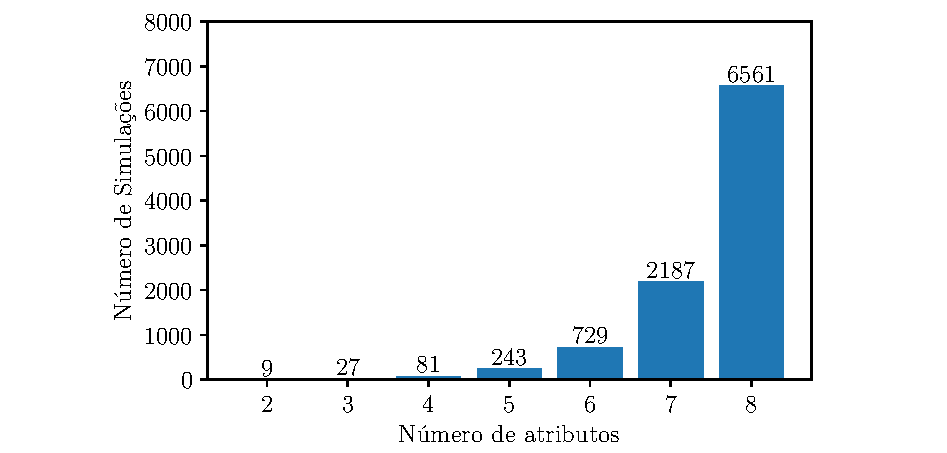
\includegraphics[scale=1]{Figuras/arvoredevr.pdf}
    \caption{Número de simulações para Àrvore de derivação com 3 níveis.}
    \legend {Fonte: Adaptado de \citeonline{madeira}}
    \label{fig:arvorederivacao2}
\end{figure}


A presença desnecessária de atributos pouco influentes incrementa o tempo computacional de processamento, devido ao aumento do número de modelos de simulação. Deste modo, os atributos que compõe a Àrvore de derivação são os definidos como críticos na análise de sensibilidade, ou seja, apenas os atributos que exercem influência significativa na Função-objetivo. Deste modo caso o número de atributos críticos seja elevado, a metodologia passa a ser custosa do ponto de vista computacional \cite{madeira}.

Após a realização das simulações e com base nos resultados, é possível realizar o tratamento estatístico necessário para obter a curva de risco de falha. Esse tratamento estatístico envolve a análise dos dados coletados durante a simulação, a determinação das probabilidades de falha em diferentes cenários e a construção da curva de risco, que representa a probabilidade de ocorrência da falha ao longo do tempo operacional. Essa curva de risco de falha é uma ferramenta valiosa para a tomada de decisões informadas e a implementação de medidas de mitigação de risco adequadas \cite{risso1}.


\subsection{Método de Monte Carlo}

O método de Monte Carlo é uma técnica estatística que envolve a amostragem aleatória de variáveis de entrada incertas. Essa abordagem é utilizada como uma ferramenta para gerar cenários diversos, nos quais são realizadas inferências estatísticas. Em outras palavras, a técnica de Monte Carlo é uma técnica para modelagem de cenários estocásticos (sujeito a alguma densidade de probabilidade). A amostragem aleatória é realizada nos atributos que exercem influência sobre o problema estudado e os valores são amostrados de acordo com sua distribuição de probabilidade de cada atributo (assumida ou estimada) \cite{hammers}.

Para o método de Monte Carlo, para cada cenário simulado, existe uma solução para o problema. Deste modo, os cenários realizados resultam em um espectro com a distribuição de probabilidades empírica das respostas. Para produzir uma estimativa consistente da função de distribuição de probabilidade para a resposta, é necessário simular um número elevado de cenários. Portanto, é imprescindível a obtenção de diversos valores aleatórios para os atributos de modo que os cenários realizados possam se adequar à distribuição dos atributos \cite{Srikanta}


As etapas do método de Monte Carlo são, basicamente:

\begin{itemize}
  \item Gerar sorteios e obter amostras de objetos estocásticos com uma determinada densidade de
probabilidade;
  \item Obter o resultado da Função-objetivo de cada cenário realizado pelos sorteios;
  \item Agregar os resultados para obter dados estatísticos para análise;
  \item Assegurar que os resultados são representativos, ou seja, evidenciar o número de sorteios ideal que reproduzam de maneira fiel a distribuição dos atributos e que as estatísticas da resposta permaneçam dentro de uma margem de erro aceitável.
\end{itemize}

A simulação numérica por fluidodinâmica computacional para previsão do desgaste erosivo dos cenários gerados pela técnica de Monte Carlo é inviável do ponto de vista computacional, devido ao elevado número de sorteios. Por esta razão, é necessário recorrer a metodologias que resultem nas respostas com menor esforço computacional e estatisticamente confiável em relação ao modelo de simulação numérico. Assim, os metamodelos (\textit{Proxy models} ou \textit{Surrogate models}) se apresentam como uma excelente alternativa à simulação de Monte Carlo como ferramenta subsidiária da metodologia. Os metamodelos são aplicados para substituirem modelos de simulação numérica e podem ser usados para diminuição do esforço e tempo computacional empregados para análise de risco. Na próxima seção são abordados os métodos de geração de metamodelos através da metodologia de Superfície de Resposta.
%%%%%%%%%%%%%%%%%%%%%%%%%%%%%%%%%%%%%%%%%%%%%%%%%%%%%%%%%%%%%%%%%%%%%%%%%%%%%%%%%%%%%%%%%%%%%%%%%%%%%%%%%%%%%%%%%%%

\section{Metamodelos}

As Simulações fluidodinâmicas para previsão de desgaste erosivo, necessitam de muito esforço computacional, principalmente nos processos de análise de risco que demandam diversos cenários probabilísticos.
Os metamodelos (\textit{Proxy models} ou \textit{Surrogate models}), portanto, se apresentam como ferramentas subsidiárias da análise de risco, com objetivo de reduzir o número de simulações requisitadas para elaboração e previsão dos cenários probabilísticos necessários para composição das curvas de risco de falha por desgaste erosivo.
Neste trabalho, o planejamento estatístico é aplicado em duas ocasiões. Inicialmente o seu emprego tem como finalidade realizar a triagem dos atributos incertos, determinando quais fatores apresentam maior influência na função-objetivo, com objetivo de reduzir o número de simulações necessárias nas etapas seguintes de análise \cite{Lih}.

A segunda aplicação do planejamento de experimentos é a elaboração de modelos de simulação planejados, os quais são resultam na elaboração da Superfície de resposta. Esta metodologia permite a obtenção de um modelo que inclue os termos significativos estatisticamente no desgaste erosivo, que pode substituir o simulador de fluxo para obtenção da curva de risco do estudo. 


\subsection{Planejamentos Estatísticos e Superfície de Resposta}


Um planejamento estatístico, também conhecido como planejamento de experimentos, se caracteriza por um conjunto de ensaios em que são realizadas alterações nas variáveis de entrada e são observadas as alterações na variável de resposta do processo \cite{myers}. Portanto, as alterações nos parâmetros de entrada são previamente planejadas, ou seja, o trabalho estatístico mais importante consiste na maneira em que os dados são obtidos. A primeira etapa compreende a definição dos objetivos a serem alcançados, para escolha correta do tipo de planejamento estatístico a ser aplicado. Em seguida devem ser definidos os parâmetros, as faixas de variação e a variável de resposta do experimento. 

Com o avanço da tecnologia, a capacidade de processamento computacional cresceu, e foram desenvolvidos diversos sistemas computacionais para a simulação de fenômenos físicos complexos. Devido ao alto tempo e custo computacional que técnicas avançadas de simulação demandam, muitas setores da indústria e pesquisa aderiram às técnicas de design experimental para substituição dos simuladores. Na indústria petrolífera, o planejamento estatístico foi introduzido na década de 90 no trabalho de \citeonline{damsleth}, aplicando-o em conjunto com simulação numérica de reservatórios para estimar as incertezas na previsão de produção para definição de estratégias de drenagem para o desenvolvimento de um campo petrolífero no Mar do Norte. No trabalho de \citeonline{yeten} foi realizado um estudo comparando vários designs experimentais e metodologias de superfície de resposta aplicadas em uma etapa de análise de sensibilidade. O qual demonstrou precisão do modelo gerado pelo planejamento de experimentos em comparação com o simulador. O estudo de \citeonline{slotte}, aplicou o Planejamentos estatísticos para experimentos simulados com intuito de substituir o simulador de fluxo, o qual demonstrou que é possível construir funções matemáticas precisas o suficiente para descrever a função de distribuição de probabilidade da resposta (PDF) e, assim, avaliar a incerteza associada aos modelos de reservatórios petrolíferos.

No processo de planejamento de experimentos, geralmente, não se tem o conhecimento das variáveis que afetam significativamente a variável de resposta. Deste modo, é necessário um estudo prévio com o máximo possível de variáveis para que se obtenha as variáveis que mais impactam na resposta dos ensaios simulados. O entendimento das variáveis significativas, contribui para a execução do planejamento para obtenção de Superfície de resposta, por garantir que apenas as variáveis que exercem impacto significativo, sejam utilizadas na elaboração da matriz de experimentos. A triagem das variáveis pode ser realizada por planejamentos fatoriais ou pelo método de análise de sensibilidade. O método de análise de sensibilidade se baseia na utilização da simulação de fluxo de um modelo base, com valores de maior probabilidade dos atributos aleatórios. A partir do modelo base, os atributos incertos são variados em níveis (-1, 0 e 1), com finalidade de observar o impacto de cada parâmetro na alteração da função-objetivo (variável de resposta) \cite{risso1}.

O planejamento fatorial de Plackett-Burman é uma abordagem que permite estimar os efeitos principais de cada variável individualmente, considerando os efeitos de interação como irrelevantes. Essa metodologia é vantajosa, pois reduz significativamente o número de ensaios necessários em comparação com outros tipos de planejamento experimental. Ao realizar o planejamento fatorial de Plackett-Burman, é importante que o número de ensaios seja maior do que a quantidade de variáveis. Isso garante que haja graus de liberdade suficientes para o cálculo do erro padrão e a identificação dos fatores estatisticamente relevantes. O número de ensaios deve ser cuidadosamente escolhido para fornecer informações confiáveis e significativas sobre os efeitos das variáveis estudadas, permitindo a análise estatística adequada \cite{plackett}. A Tabela \ref{tab:plackettburmanmatriz} demonstra o planejamento fracionário do tipo Plackett & Burman para estimar a influência de quatro fatores na função-objetivo. 


\begin{table}[!h]
\caption{Exemplo de matriz do planejamento Plackett-Burman para 4 variáveis.}
\begin{tabular*}{\textwidth}{@{\extracolsep{\stretch{1}}}*{6}{c}@{}}
 \toprule
   Ensaio&x1& x2& x3& x4& Função-Objetivo\\
  \midrule
1&-1&-1&-1&1&Fo1\\
2&1&1	&1&-1&Fo2\\
3&-1&	1&		-1&		-1&Fo3\\
4&-1&		-1&		1&		1&Fo4\\
5&1&		-1&		1&		1&Fo5\\
6&-1	&	-1&		-1&		-1&Fo6\\
7&-1&		1&		1&		1&Fo7\\
8& 1&		-1&		1&		-1&Fo8\\
9&-1&		1&		1&		-1&Fo9\\
10&1&		1&		-1&		1&Fo10\\
11& 1&		1&		-1&		1&Fo11\\
12&1	&	-1&		-1&		-1&Fo12\\

  \bottomrule   
\end{tabular*}
\label{tab:plackettburmanmatriz}
\end{table*}
\end{table}

A metodologia de Superfície de Resposta é um conjunto de técnicas para modelagem de processos cuja função-objetivo, é influenciada por diversos atributos. Na metodologia de análise de risco a superfície de resposta é aplicada, principalmente, para gerar metamodelos (\textit{Proxy models} ou \textit{Surrogate models}) que substituam o simulador de fluxo numérico que resultam em menor custo e eficiência na previsão de novos valores \cite{risso1}. O planejamento de \citeonline{box} é comumente aplicado para procedimentos de obtenção de metamodelos. Esta metodologia é considerada proficiente, pois é capaz de gerar superfícies de resposta de ordem superior usando menos execuções necessárias do que outras técnicas, como a Fatorial completa e de Composto Central. O planejamento de experimentos \citeonline{box} consiste em aplicar 3 níveis para os atributos que influenciam na função-objetivo com intutito de gerar a Superfície de resposta. A matriz do planejamento consiste em posicionar os pontos no centro das arestas do cubo e um ponto no centro do hiperespaço (Figura \ref{fig:cubo}), diferentemente do que ocorre nos Planejamentos Fatoriais em que os pontos se situam nos vértices. 

\begin{figure}[H] 
    \centering  
    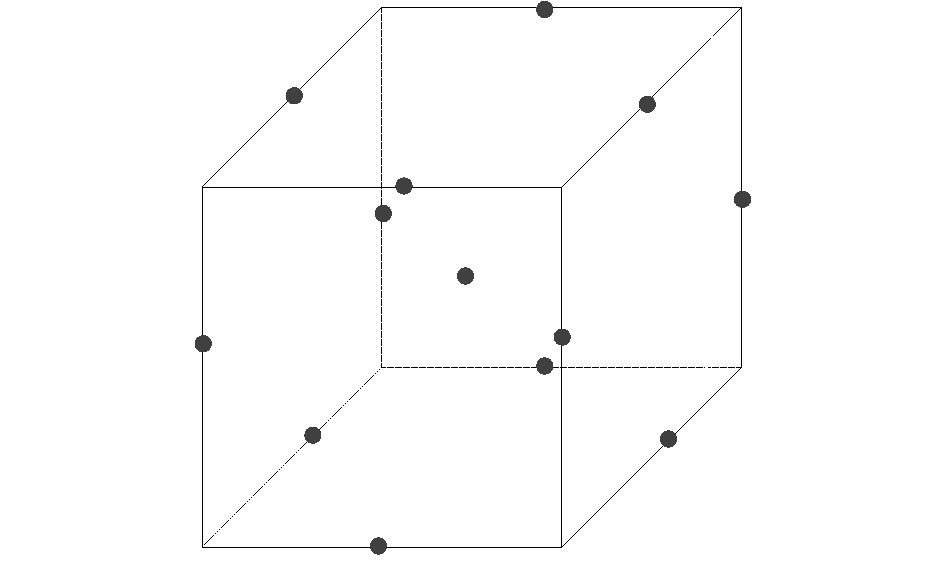
\includegraphics[scale=0.65]{Figuras/cubo.pdf} 
    \caption{Planejamento de Box Behnken.}  
    \legend{Fonte: Adaptado de \citeonline{FERREIRA2007179}}
    \label{fig:cubo}  
\end{figure}

Através da configuração da matriz de Box Behnken é possível obter a Superfície de reposta com os termos lineares, termos com interação e termos quadráticos. Os pontos fatoriais da matriz presentes nas arestas são responsáveis por fornecerem as informações para modelagem de primeira ordem, obtendo os termos lineares e de interações do sistema. Por outro lado, os pontos centrais permitem estimativas dos termos
termos quadráticos da superfície de resposta. O número total de simulações realizadas para a matriz de Box Behnken é \textit{N = 2 * k * (k $-$ 1) + Co}, em que \textit{k} é o número de atributos e \textit{Co} é o número de pontos centrais \cite{box}. 

Através das combinações de atributos geradas a partir da matriz de Box Behnken são efetuadas simulações fluidodinâmicas, o que possibilita a obtenção das respostas da função-objetivo. Após a obtenção da matriz completa com as respectivas respostas, é efetuada a obtenção dos coeficientes de regressão e avaliação estatística dos termos do modelo.

A análise dos termos para os planejamentos estatísticos (Box Behnken e Plackett Burmann) é realizada através de validação estatística, por meio da tabela ANOVA (Análise de variância). Os termos lineares, de interação e quadráticos são considerados significativos para a função-objetivo caso apresentem significância estatística, através do teste \textit{p} e teste F de Fischer presentes na Análise de variância. O teste \textit{p} é um método estatístico que testa a validade da hipótese nula acerca de uma população. Quanto menor o valor-\textit{p}, maior a evidência que a hipótese nula deve ser rejeitada e que a hipótese alternativa pode ser mais confiável. Comumente os níveis alfa são definidos em 5\% ou menos, que se traduzem em intervalos de confiança de 95\% ou mais. Em outras palavras, um valor-\textit{p} inferior a um nível alfa de 5\% significa que existe mais de 95\% de chance de que os resultados não sejam aleatórios e sejam, de fato, significativos estatisticamente. 

A fim de verificar se o modelo se ajusta bem aos dados, são examinadas diversas medidas de adequação. Uma das premissas de um modelo de regressão é a de que os resíduos do modelo devem seguir uma distribuição normal \cite{montgomery}. Para tanto, o teste de normalidade de Kolmogorov-Smirnov é utilizado para avaliar a adequação dos resíduos dos modelos a uma distribuição normal. A hipótese nula deste teste é que os resíduos seguem uma distribuição normal, enquanto a hipótese alternativa é que não seguem. Deste modo, o valor-p resultante é comparado com um nível de significância de 0,05 para determinar se a hipótese nula pode ser rejeitada ou não. Se o valor-p for maior que 0,05, os resíduos são considerados adequados para uma distribuição normal. Caso contrário, os resíduos não são considerados adequados para uma distribuição normal.

Outra análise necessária para o modelo de regressão é a de homocedasticidade dos resíduos do modelo. A homocedasticidade é uma característica estatística que se refere à igualdade da variância dos erros em um modelo estatístico em toda a amplitude dos valores preditores, ou seja, das variáveis independentes. Em outras palavras, a homocedasticidade indica que a dispersão dos erros em torno da linha de regressão é constante em todos os níveis da variável independente. É uma suposição importante em muitos modelos estatísticos, incluindo análises de regressão. Pois a falta de homocedasticidade pode levar a estimativas imprecisas e tendenciosas. Uma maneira comum de avaliar a homocedasticidade é através de gráficos de dispersão dos resíduos em relação às variáveis independentes, onde uma distribuição uniforme sugere homocedasticidade e uma tendência clara dos resíduos indica heterocedasticidade \cite{myers}.

No teste F de Fischer, os valores calculados F para os termos do modelo são comparados com os valores F tabelados de uma distribuição de referência, de acordo com um nível alfa, comumente definido em 5\% e um intervalo de confiança de 95\%. Portanto, um termo é considerado significativo para a variável de resposta do modelo se o F calculado do termo for maior que o F tabelado em um determinado intervalo de confiança e para um determinado Grau de liberdade.


% \subsection{Aprendizado de máquina \textit{(Machine Learning)}} 

% Aprendizado de máquina (ML), são recursos computacionais para desenvolver reconhecimento de padrões, de forma automatizada, a partir de dados de entrada. Os modelos computacionais são desenvolvidos com o objetivo de adquirir informação, realizar inferências e tomar decisões a partir de conjuntos de dados através de métodos estatísticos. Uma característica notável da modelagem de aprendizado de máquina é lidar com problemas multivariados, ou seja, que envolvem diversas variáveis em diferentes escalas \cite{shalev}. Os métodos de aprendizado de máquina podem ser categorizados em: aprendizado supervisionado, aprendizado não supervisionado e aprendizado por reforço.  


% \subsubsection{Aprendizado de máquina supervisionado}  

% Os métodos de aprendizado supervisionado, que é foco desse trabalho, incluem algoritmos que coletam amostras de dados (dados de treino) e suas saídas associadas (\textit{output} ou resposta) para gerar o treinamento do modelo computacional. Esses métodos são chamados de supervisionados, pois o modelo aprende a partir de amostras de dados onde as respostas de saída (\textit{output}) são conhecidas antes de iniciar o processo de modelagem. O objetivo principal é desenvolver um mapeamento ou associação entre amostras de dados de entrada “x” e suas saídas correspondentes “y” com base em várias instâncias de dados de treino. Os modelos podem posteriormente ser usados para a predição do valor do atributo alvo para qualquer nova amostra de dados de entrada \cite{sbsi}. Existem diversos algoritmos de aprendizado supervisionado, tais como: \textit{ Random Forest (RF), Support Vector Machines (SVM), K-Nearest Neighbor (KNN), Decision Tree (DT), Catboost (CB)}, entre outros.  

% Os métodos de aprendizagem supervisionada possuem duas classes principais chamadas de Classificação e Regressão. A aprendizagem supervisionada por classificação possui objetivo principal de prever respostas de natureza categórica para os dados de entrada, com base no que o modelo aprendeu na fase de treinamento. Ou seja, cada resposta de saída do modelo pertence a uma classe ou categoria discreta específica. O método de aprendizagem supervisionada por regressão, é caracterizado por modelos de ML treinados em amostras de dados de entrada em que as respostas são valores numéricos e contínuos. Os modelos de regressão fazem uso de atributos ou recursos de dados de entrada (também chamados de variáveis explicativas ou independentes) e suas valores de saída numéricos e contínuos\cite{james}.  

% \subsubsection{Amostragem de dados por hipercubo latino}  

% Algumas etapas deste trabalho requerem o treinamento de algoritmos de Machine Learning, para tanto é necessário a geração de amostras de dados, ou seja, dados de treino que possuam as respostas do processo que se objetiva modelar. O Hipercubo Latino é um método de amostragem de números aleatórios que visa distribuir a obtenção de amostras de forma uniforme sobre o espaço amostral, ou seja, a seleção de valores aleatórios é realizada de forma dependente \cite{mackay}. A distribuição do atributo é dividia em n regiões diferentes, com igual probabilidade de ocorrência, e seleciona aleatoriamente um valor de cada região para obter uma amostra de tamanho n (Figura \ref{fig:hipercubolatino}).  


% \begin{figure}[H] 
%     \centering  
%     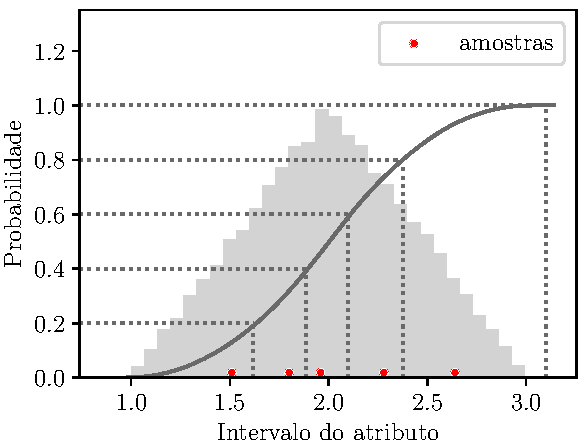
\includegraphics{Figuras/hipercubolatino.pdf}  
%     \caption{Amostragem por Hipercubo Latino.}  
%     \legend{Fonte: Adaptado de \citeonline{mackay}.}
%     \label{fig:hipercubolatino}  
% \end{figure}

% No exemplo mostrado na Figura \ref{fig:hipercubolatino}, para obtenção de 5 amostras de um determinado atributo incerto, a distribuição foi dividida em 5 estratos de igual probabilidade e em cada estrato obtido um valor aleatório. Portanto, conforme o número de amostras aumente, a faixa de valores obtidos por amostragem fica mais próxima da distribuição original.

% \subsubsection{Métodos \textit{ensemble}}


%   Os métodos de aprendizado de máquina \textit{ensemble} são técnicas que criam vários modelos e depois os combinam de alguma forma para produzir melhores resultados. Os métodos de conjunto geralmente produzem soluções mais precisas do que um único modelo. Estes métodos surgiram pois em muitos casos modelos que possuem bons resultados em dados de treinamento, nem sempre oferecem bom desempenho para previsão de novos dados (desconhecidos). Deste modo, a combinação de modelos base podem aumentar a probabilidade de predições satisfatórias em novos dados que não se assemelham aos de treinamento \cite{polikar}. Existem diversos métodos ensemble para combinação de algoritmos, como por exemplo: \textit{bagging, boosting e voting.}

% O método \textit{bagging} divide o conjunto de dados em subconjuntos para treinamento de diferentes algoritmos. Deste modo, para uma modelagem de classificação, a predição da maioria dos modelos é definida como resultado do modelo \textit{ensemble}. No caso de modelagem de regressão, é obtida a média do resultado de todos modelos como predição final para o modelo ensemble. O \textit{Random Forest} é um método de \textit{bagging} com algumas especificidades, que utiliza Árvores de decisão para predição (Figura \ref{fig:randomforest}). De acordo com \cite{breiman}, o método de \textit{Random Forest} utiliza Árvores de decisão distintas para cada subamostragem do conjunto de dados, com objetivo de combinar seus resultados para melhor estimativa de predição final.

% \begin{figure}[H] 
%     \centering  
%     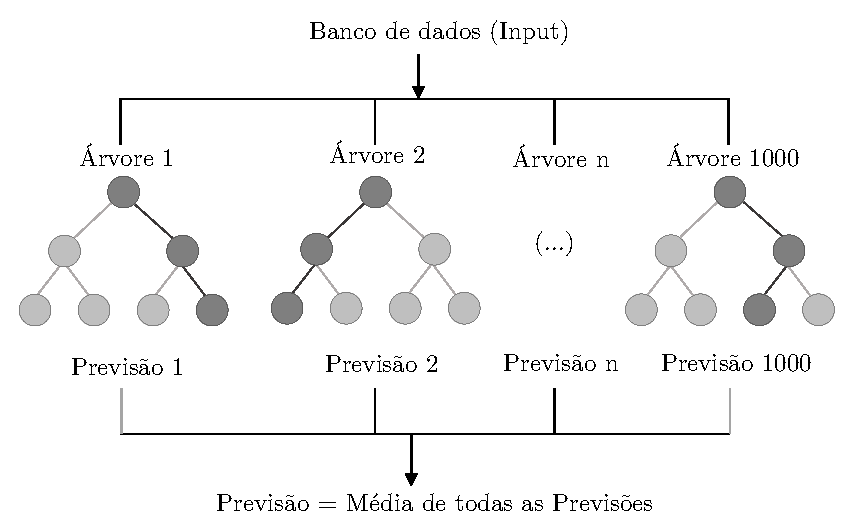
\includegraphics{Figuras/random forest.pdf}  
%     \caption{Método Bagging de regressão por Random Forest.}  
%     \legend{Fonte: Adaptado de \citeonline{breiman}.}
%     \label{fig:randomforest}  
% \end{figure}


% O método de \textit{boosting} treina os modelos de aprendizado de máquina em diferentes dados de treinamento, assim como no método de \textit{bagging}.  Porém, os modelos utilizados no \textit{boosting} aprendem sequencialmente, ou seja, cada algoritmo busca minimizar os erros do modelo anterior. Deste modo, modelos fracos contribuem para criação de modelos preditores mais eficazes, conforme demonstrado na Figura \ref{fig:boosting}. Diferentemente dos modelos \textit{bagging}, a predição de cada algoritmo é ponderada com base em seu desempenho, deste modo os modelos não possuem o mesmo peso na predição final. Existem diversos algoritmos que se baseiam no método de \textit{boosting}, como Catboost, Adaboost, LightGBM, XGBoost entre outros \cite{chen2016}.

% \begin{figure}[H] 
%     \centering
%     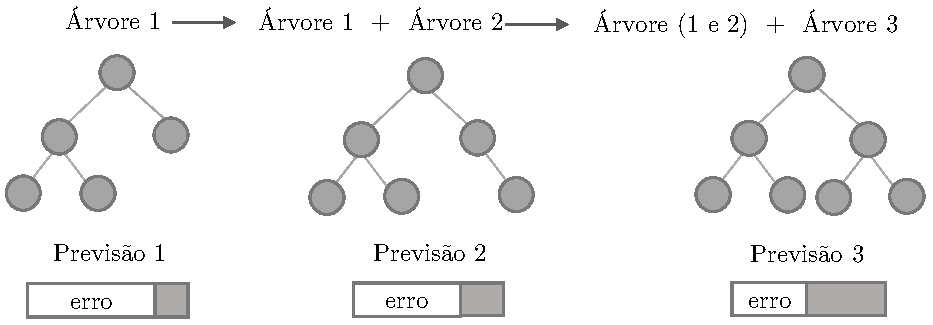
\includegraphics{Figuras/boosting.pdf}
%     \caption{Método Boosting de regressão pelo algoritmo Catboost.}
%     \label{fig:boosting}
%     \legend{Fonte: Adaptado de \citeonline{chen2016}.}
% \end{figure}

% Os métodos de \textit{voting}, podem combinar modelos de diferentes algoritmos para realizar predições. Ao contrário dos modelos de \textit{boosting} e \textit{bagging} que necessitam de modelos de um mesmo tipo. Deste modo, algoritmos diferentes como Support Vector Machines e Árvores de decisão podem ser combinados para realizar uma predição, por exemplo. O resultado final é baseado na maioria dos votos dos algoritmos utilizados \cite{yaman2018}.


% \subsubsection{Aprendizado de máquina automatizado (AutoML)}  

% O crescente uso do aprendizado de máquina em aplicações trouxe consigo a necessidade de automatizar cada vez mais as tarefas de desenvolvimento, visando simplificar as etapas de pré-processamento de dados e criação de modelos preditivos e tornar a prática de aprendizado de máquina mais eficiente. O aprendizado de máquina automatizado (AutoML) é o processo de automatizar as tarefas de aplicação do aprendizado de máquina que seleciona automaticamente os algoritmos para a criação de modelos e quais hiperparâmetros devem ser ajustados para melhorar o desempenho da máquina. O AutoML inclui potencialmente todos os estágios, desde o início com um conjunto de dados brutos até a criação de um modelo de aprendizado de máquina pronto para implantação \cite{balaji2018}. Automatizar o processo de aplicação de aprendizado de máquina oferece as vantagens de produzir soluções mais simples, criação mais rápida dessas soluções e modelos que geralmente superam os modelos projetados de forma padrão. Existem algumas bibliotecas na linguagem Python de código aberto para o \textit{pipeline} de desenvolvimento que oferecem estruturas de autoML para preparações de dados em modelos adaptáveis. Esses \textit{frameworks} automatizam, por exemplo, imputações de valores ausentes, transformações de dados, ajustes de hiperparâmetros e avaliação dos resultados com métricas específicas \cite{elshawi2019}. 

% O PyCaret é um \textit{framework} de aprendizado de máquina e gerenciamento de modelos de código aberto em linguagem de programação Python que automatiza fluxos de trabalho, o que reduz o tempo dedicado na programação de códigos. O PyCaret é essencialmente um compilado em Python de várias bibliotecas e estruturas de aprendizado de máquina que incluem os algoritmos tradicionais e \textit{ensemble}, como scikit-learn, XGBoost, LightGBM, CatBoost, spaCy, Optuna, Hyperopt, Ray entre outras. Comparado com outras bibliotecas de aprendizado de máquina de código aberto, o PyCaret é uma alternativa que pode ser usada para substituir centenas de linhas de programação por apenas alguns comandos. Isso torna os projetos exponencialmente rápidos e eficientes \cite{iqbal2021}.   


\subsubsection{Métricas de Desempenho dos modelos de regressão}  


As métricas de desempenho são cálculos realizados com objetivo de analisar a capacidade preditiva de modelos de regressão. Para modelagens em que os atributos de resposta apresentam variável numérica e contínua, o RMSE é uma métrica frequentemente utilizada. Seu cálculo consiste na raiz quadrada da média dos erros quadrados, entre os valores reais e os previstos pelo modelo, de acordo com a equação \ref{eqn:rmse}.  Quanto maior o valor de RMSE, pior o modelo preditivo.  

  
\begin{equation} 
RMSE = \left ( \frac{1}{n} \sum_{i=1}^{n} ({yi}-\hat{yi})^2 \ \right )^{1/2}  
    \label{eqn:rmse} 
\end{equation} 

Onde:

yi= valor verdadeiro;

$\hat{yi} = \textrm{valor previsto};$

n= tamanho da amostra.

\vspace{1cm}

O cálculo da métrica RMSE eleva a média dos erros do modelo ao quadrado. Assim, diferenças que sejam menores apresentam menor impacto no cálculo, enquanto diferenças maiores recebem mais peso. Outra métrica de regressão amplamente utilizada é o MAE, demonstrado na equação \ref{eqn:mae}. A equação atribui o mesmo peso a todas as diferenças, pois não são elevadas ao quadrado. Deste modo, diferenças grandes e pequenas apresentam o mesmo peso no cálculo da métrica.  


\begin{equation} 
    MAE = \frac{1}{n} \ \sum_{i=1}^{n} | yi - \hat{yi}|  
    \label{eqn:mae} 
\end{equation} 

Onde:

yi= valor verdadeiro;

$\hat{yi} = \textrm{valor previsto};$

n= tamanho da amostra.
\vspace{1cm}

% O MAPE é uma métrica que calcula a média percentual do desvio absoluto entre as predições e os dados observados (equação \ref{eqn:mape}). Essa medida fornece um valor porcentual da média que do quanto o modelo erra nas previsões. Por exemplo, um modelo de regressão com MAPE de 20\% significa que, em média, as previsões erram em 20\% do valor verdadeiro. Ou seja, quanto menor o valor, mais preciso é o modelo de regressão.  

  

%   \begin{equation} 
%       MAPE = \frac{1}{n} \ \sum_{i=1}^{n} | \frac{yi - \hat{yi}}{yi}|  
%       \label{eqn:mape} 
%   \end{equation} 
  

% Onde:

% yi= valor verdadeiro;

% $\hat{yi} = \textrm{valor previsto};$

% n= tamanho da amostra.


% \vspace{1cm}
  Outra métrica comum é o coeficiente de determinação R². Que consiste em uma medida estatística que representa a proporção da variância de uma variável dependente que é explicada por uma variável ou variáveis independentes em um modelo de regressão (equação \ref{eqn:r2}). O R² explica até que ponto a variância de uma variável explica a variância da uma segunda variável. 
  
  \begin{equation}
      R^{2}= 1 - \frac{\sum yi-\hat{yi}}{\sum yi - \overline{y}}
      \label{eqn:r2} 
  \end{equation}


Onde:

yi= valor verdadeiro;

$\hat{yi} = \textrm{valor previsto};$

\={y} = \textrm{média}.$



\include{Capitulos/Cap3-Revisaobibliografica}
\chapter{Materiais e Métodos}


A metodologia proposta neste trabalho visa a aplicação de técnicas de quantificação
de risco de um projeto hipotético de poço petrolífero na fase de perfuração. As abordagens propostas para quantificação de risco consistem na utilização das metodologias da Árvore de derivação e de Monte Carlo, que por sua vez, estão subsidiadas pela aplicação de Planejamento estatístico para geração de metamodelos (\textit{Proxy models} ou \textit{Surrogate models}), que possam substituir o simulador fluidodinâmico na quantificação do desgaste erosivo em cenários que demandam muitas simulações.
A metodologia de análise de risco é focada na geração de diversos cenários possíveis de fluxo, compostos pela combinação dos atributos incertos que influenciam na resposta de desgaste erosivo através dos métodos de Árvore de Derivação (AD) e Monte Carlo (MC). As principais etapas desta metodologia são:

\begin{itemize}
  \item Escolha dos atributos incertos que influenciam no desgaste erosivo segundo estudo bibliográfico;
  \item Definição das distribuições de probabilidades das variáveis aleatórias e probabilidades de ocorrência associadas a cada nível discretizado;
  \item Triagem e seleção dos atributos críticos, ou seja, que exercem maior impacto no desgaste erosivo, através da Análise de sensibilidade e Planejamento Plackett Burmann;
  \item Geração de metamodelo através de Planejamento estatístico Box Behnkhen para previsão do desgaste erosivo em substituição ao simulador numérico;
  \item Geração de cenários de simulação através da combinação dos atributos críticos através das técnicas de Àrvore de derivação Monte Carlo;
  \item Obtenção da curva de risco das funções-objetivo através do tratamento estatístico e
obtenção dos percentis P10, P50 e P90. 
\end{itemize}

\section{Variáveis aleatórias e distribuições de probabilidades}
\label{cap:Variáveis aleatórias e distribuições de probabilidades}

 Para obter a análise de risco de um projeto, são necessárias amostragens das variáveis aleatórias que influenciam no fenômeno estudado. Os atributos que influenciam no desgaste erosivo, segundo a literatura, foram expostos no capítulo \ref{cap:Erosão por partículas sólidas}. Para esta dissertação, as variáveis aleatórias consideradas para as previsões de desgaste erosivo foram: Tamanho do cascalho, Forma do cascalho, Densidade do cascalho, Densidade do fluido de perfuração, Viscosidade do fluido de perfuração, Velocidade de escoamento e Vazão mássica (Figura \ref{fig:erosaoatb2}). 

\begin{figure}[H] 
    \centering  
    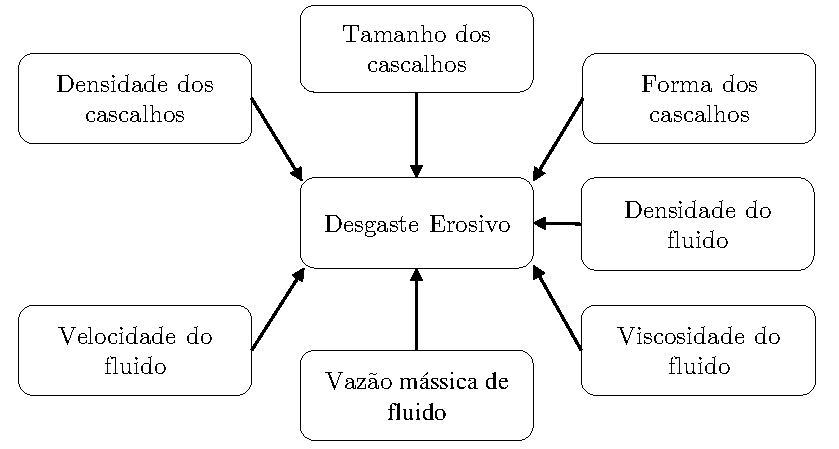
\includegraphics{Figuras/erosaoatb2.pdf}  
    \caption{Relação das variáveis aleatórias consideradas para análise de risco de falha.}  
    \legend{Fonte: o autor.}
    \label{fig:erosaoatb2}  
\end{figure}

As variáveis relativas à propriedade do material alvo não foram consideradas variáveis aleatórias neste estudo (Dureza, Microestrutura) pois apenas a curva de Aço Carbono de 90º e suas propriedades são consideradas na análise de desgaste erosivo. 

A aquisição de dados e amostragens de perfuração é muito dificultosa, uma vez que a maioria das informações obtidas pelas operadora petrolíferas, geralmente, são tratadas com sigilo. Além disso, a obtenção de algumas informações demandam altos investimentos e tempo para serem coletadas. De posse de dados reais, são realizados testes de aderência para caracterizar a distribuição de frequência das variáveis segundo testes estatísticos. Portanto, diante do exposto, para aplicação da metodologia de análise de risco, os dados utilizados nesta dissertação são sintéticos e fictícios, ou seja, as distribuições das variáveis aleatórias foram elaboradas para este estudo de caso hipotético. Os intervalos das distribuições contínuas geradas para o trabalho foram baseadas em valores mínimos, médios e máximos de acordo com a literatura \cite{bortotti} \cite{santoss2} \cite{pereira}, através destes valores foram geradas distribuições de probabilidades (gamma, normal, lognormal e triangular) para representação amostral das variáveis aleatórias. 

Após definição das distribuições de probabilidade, foram discretizados os níveis de incerteza, os valores de cada atributo e as probabilidades de ocorrência associada a cada nível, relacionados na Tabela \ref{tab:atributos}. Foi admitida total independência entre os atributos, ou seja, todas as combinações de atributos na construção de um modelo de fluxo multifásico para análise de erosão são possíveis.

 Os atributos incertos foram discretizados em três níveis de acordo com as respectivas distribuições de probabilidade geradas, com intuito de realizar as metodologias de análise de risco por Árvore de derivação, os planejamentos estatísticos subsequentes, para determinação do impacto dos atributos na taxa erosiva e para criação do metamodelo de regressão através da metodologia de Superfície de resposta. O nível "0" representa o valor mais provável do atributo, o nível "–1" configura o nível inferior e o nível "1" descreve o nível superior da discretização de cada variável aleatória. A Figura \ref{fig:discretizacao} demonstra, como exemplo, a função de distribuição de probabilidade da variável de "Forma dos cascalhos" e sua discretização em diferentes níveis com probabilidades associadas.

\begin{figure}[H] 
    \centering  
    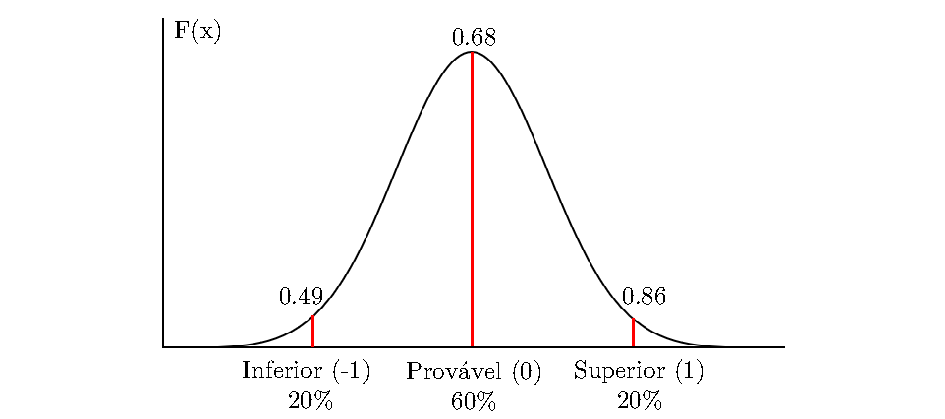
\includegraphics{Figuras/discretizacao.pdf}  
    \caption{Função de distribuição de probabilidade da variável aleatória Forma dos cascalhos de perfuração}  
    \legend{Fonte: o autor.}
    \label{fig:discretizacao}  
\end{figure}

A Figura \ref{fig:discretizacao} ilustra a distribuição de tipo normal aplicada à variável "Forma dos cascalhos". Cabe ressaltar que a distribuição normal atribuida a esta variável aleatória não apresentou valores negativos. Neste exemplo, podemos observar o processo de discretização da variável aleatória em três níveis distintos (-1= 0.49; 0= 0.68; 1= 0.86), que desempenha um papel fundamental para possibilitar as etapas de Planejamento de experimentos e Análise de risco, proporcionando uma melhor compreensão do comportamento das variáveis e seus efeitos no estudo em questão. Essa abordagem de discretização foi aplicada de forma semelhante às outras variáveis, considerando as respectivas funções de densidade de probabilidade, conforme descrito na Tabela \ref{tab:atributos}. Ao seguir essa lógica, é possível realizar análises mais detalhadas e precisas, 


\begin{table}[h]
\caption{Distribuição, níveis e probabilidades das variáveis aleatórias consideradas nesta dissertação.} 
    \begin{tabularx}{\textwidth}{llcc}
     \toprule
Atributo&Tipo de distribuição&Níveis&Probabilidades\\
  
    \midrule
    \multirow Tamanho do cascalho & Contínua (triangular)& 0 = 0.55 mm&0.60\\
    && -1 = 0.24 mm&0.20 \\
    && 1 = 0.86 mm &0.20\\
    
   \midrule
    \multirow Forma do cascalho & Contínua (normal)& 0 = 0.49 shpt&0.60\\
    && -1 = 0.68 shpt&0.20 \\
    && 1 = 0.86 shpt &0.20\\

    \midrule
    \multirow Densidade do cascalho & Contínua (gamma)& 0 = 2650 kg/m³&0.60\\
    && -1 = 2350 kg/m³&0.20 \\
    && 1 = 2950 kg/m³ &0.20\\

     \midrule
    \multirow Densidade do fluido & Contínua (lognormal)& 0 = 1375 kg/m³&0.60\\
    && -1 = 1250 kg/m³&0.20 \\
    && 1 = 1500 kg/m³ &0.20\\

    \midrule
    \multirow Viscosidade do Fluido & Contínua (triangular)& 0 = 25 cP&0.60\\
    && -1 = 15 cP&0.20 \\
    && 1 = 35 cP &0.20\\

 \midrule
    \multirow Velocidade de escoamento & Contínua(triangular)& 0 = 8.87 m/s&0.60\\
    && -1 = 9.50 m/s&0.20 \\
    && 1 = 10.13 m/s &0.20\\

    \midrule
    \multirow Vazão mássica & Contínua(triangular)& 0 = 0.13 kg/s&0.60\\
    && -1 = 0.20 kg/s&0.20 \\
    && 1 = 0.27 kg/s&0.20\\
    
    \bottomrule   
    
    \end{tabularx}
    \label{tab:atributos}
 \subcaption{Forma do cascalho (shpt) = relação entre a área da partícula e seu perímetro.}
\legend {Fonte: o autor.}
\end{table*}
\end{table}


\section{Modelo de Simulação Fluidodinâmica computacional}

Para obter quantitativamente o valor da taxa erosiva nos diversos cenários aplicados a este estudo, para emprego da análise de risco, foi necessário a elaboração de um modelo de simulação numérica por fluidodinâmica computacional, o qual apresenta diversas etapas de aplicação. A metodologia de simulação fluidodinâmica segue as etapas descritas anteriormente no capítulo \ref{Simulação Fluidodinâmica computacional (CFD)}, que necessita do desenho da geometria da curva analisada, a criação da malha computacional, a escolha dos modelos e equações para a resolução numérica de fluxo de fluido e partículas, a análise de convergência física e de resíduos e a obtenção da taxa erosiva para os diversos cenários de simulação empregados para análise de risco de falha.

\vspace{1cm}


As Simulações CFD para análise de erosão em curvas de tubulação envolvem a modelagem de múltiplos fenômenos físicos, incluindo o escoamento de fluido, o transporte de partículas sólidas, a interação partícula-parede e a erosão da parede. Portanto, a simulação pode ser computacionalmente intensiva e pode levar de algumas horas a vários dias para ser concluída, dependendo da resolução da malha (mesh), da complexidade da geometria, da precisão requerida, do poder de computação disponível e do tipo de modelagem (estacionária ou dinâmica) para execução das simulações. 

A Modelagem estacionária é baseada na suposição de que a taxa de erosão é constante em uma determinada área ao longo do tempo. Esse tipo de modelagem é mais simples e requer menos dados do que a modelagem dinâmica, mas não leva em conta as variações temporais na taxa de erosão. 

A Modelagem dinâmica leva em conta as variações temporais na taxa de erosão, permitindo uma análise mais detalhada dos processos de erosão. Esse tipo de modelagem é mais complexo e requer mais dados do que a modelagem estacionária, mas é mais preciso na estimativa da taxa de erosão ao longo do tempo. 

Por se tratar de um estudo que demanda muitos cenários de simulação para elaboração dos metamodelos e das curvas de risco, a modelagem dinâmica demandaria demasiado esforço computacional e se tornaria impraticável diante dos recursos computacionais disponíveis. Deste modo este trabalho realizou simulações CFD estacionárias para obtenção dos desgastes erosivos na tubulação curva nos diversos cenários probabilísticos estudados.

A geração da geometria é uma das fases mais importantes para a concepção da simulação Fluidodinâmica computacional, pois deve caracterizar toda a região onde ocorre o escoamento e o desgaste erosivo decorrente do impacto de partículas oriundas da perfuração de camadas rochosas. Por se tratar de um estudo envolvendo linhas hidráulicas de sistemas \textit{offshore}, este equipamento foi reproduzido com os diâmetros e geometria originais em ambiente computacional, a fim de reproduzir suas características físicas. A Figura \ref{fig:cfdgeometria} demonstra o desenho em CAD (\textit{Computer aided design}) da curva de 90 graus frequentemente utilizada nas operações de perfuração de poços de acordo com a norma de práticas recomendadas para projetos e instalação de sistemas de tubulação em plataformas de petróleo offshore \cite{api14e}. 

\begin{figure}[H] 
    \centering  
    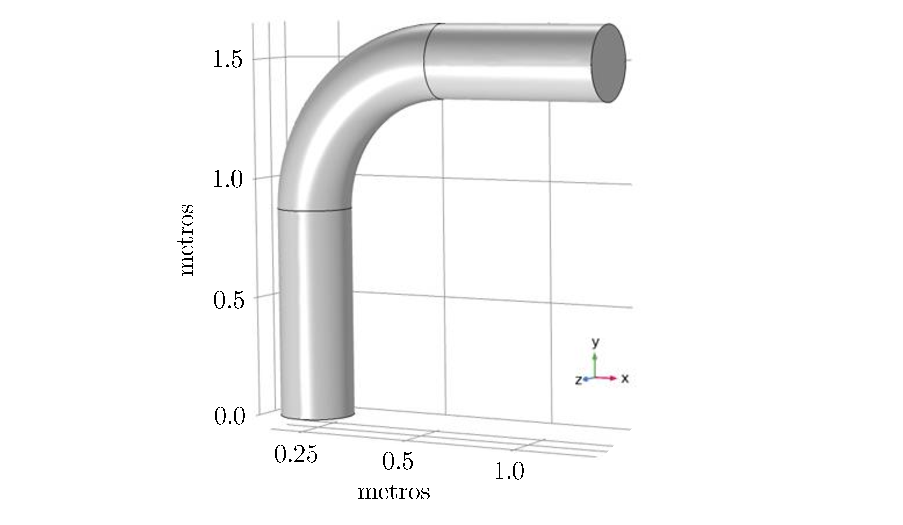
\includegraphics[width=1\textwidth]{Figuras/cfdegeometria.pdf}
    \caption{Desenho em CAD da geometria da curva de 90 graus.}  
    \legend{Fonte: o autor.}
    \label{fig:cfdgeometria}  
\end{figure}

\vspace{0.2cm}

A geometria utilizada foi de um tubo curvado de 90 graus raio
curto, de diâmetro nominal de 3 polegadas \textit{schedule} XXS. O material da curva é composto por Aço Carbono (ASTM-A 234 Gr. WPB), conforme sugerido por norma para operações em plataformas offshore \cite{api14e}. Cabe ressaltar que o material da curva influencia diretamente na magnitude do desgaste erosivo, porém a influência da geometria da curva e alteração de material não é objeto de estudo deste trabalho. Portanto, a curva de 90º de raio curto será a única avaliada para a composição da análise de risco, por ser utilizada com frequência em sistemas hidráulicos de perfuração e sugerida pela norma \cite{api14e}.

A geração da malha é uma etapa importante em simulações de CFD, com influência
direta no sucesso das simulações, entretando o número ideal de elementos de malha deve ser obtido para diminuição do tempo computacional requerido para as simulações. Para tanto, foi realizado um teste de independência da malha  para descobrir o tamanho ideal do número de elementos, com objetivo de gerar simulações de fluxo confiáveis e com custo computacional adequado (Figura \ref{fig:refmalha}).

\begin{figure}[H] 
    \centering  
    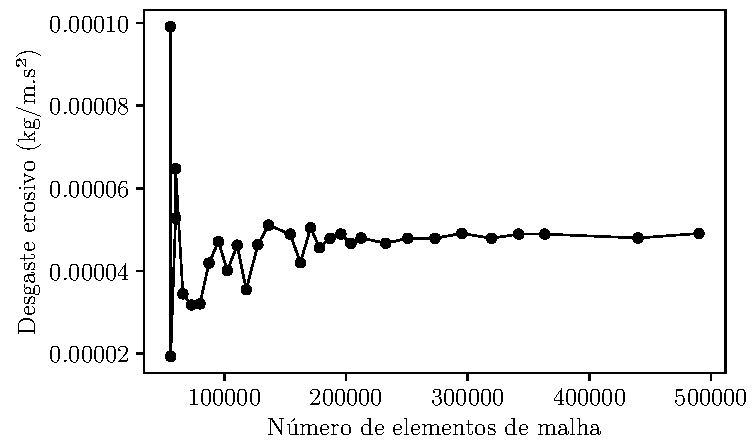
\includegraphics[textwidth=0.85\textwidth]{Figuras/testedemalha.pdf}  
    \caption{Teste de indpendência de malha para simulação fluidodinâmica computacional.}  
    \legend{Fonte: o autor.}
    \label{fig:refmalha}  
\end{figure}

É possível observar que a partir de 200.000 elementos, a solução é independente da malha. O incremento no número de elementos não influencia na resposta do dano erosivo para o modelo de simulação, ou seja, a taxa erosiva não apresentou mudanças maiores que 1\%. A Figura \ref{fig:malhaerosao} demonstra a malha computacional gerada, que compreende o total de 200.000 elementos. A malha contém elementos hexaédricos com refinamento na região de interesse para minimizar a ocorrência de elementos distorcidos \cite{zhang}.

\begin{figure}[H] 
    \centering  
    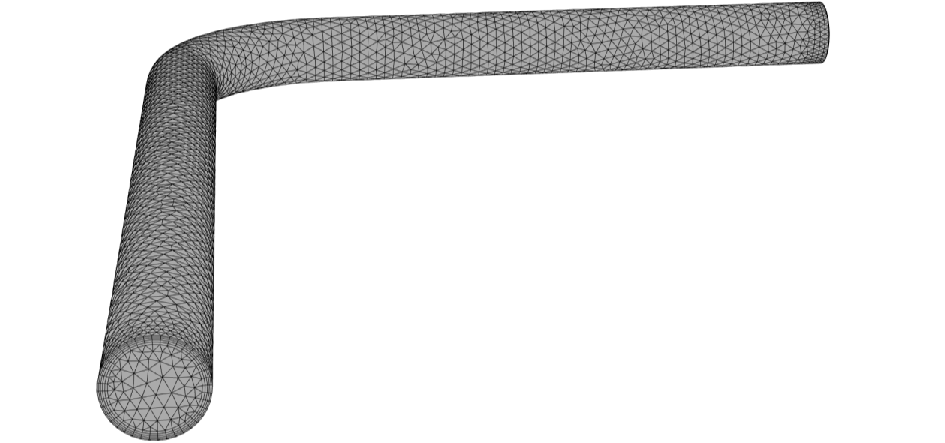
\includegraphics[textwidth=0.33\textwidth]{Figuras/MALHA.pdf}  
    \caption{Malha computacional da curva de 90 graus.}  
    \legend{Fonte: o autor.}
    \label{fig:malhaerosao}  
\end{figure}

Após criação da malha, nomeou-se as condições de contorno da curva de aço carbono (Figura \ref{fig:condcontorno}). As condições de contorno definem as regiões de entrada e saída do fluido e dos cascalhos na tubulação, e a delimitação do sistema físico através da definição da região de parede da tubulação.

\begin{figure}[H] 
    \centering  
    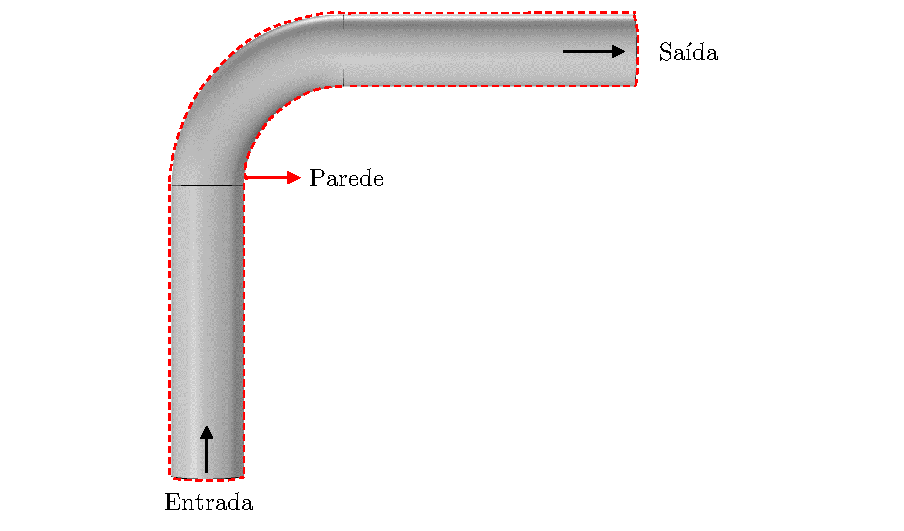
\includegraphics{Figuras/contornoregiao.pdf}  
    \caption{Condições de contorno da curva de aço carbono de 90 graus.}  
    \legend{Fonte: o autor.}
    \label{fig:condcontorno}  
\end{figure}

Para as simulações realizadas neste estudo, foi definido o regime de escoamento como permanente, o qual não considera a variação do tempo como influência direta nos atributos de entrada. A turbulência foi modelada utilizando  as equações de k-e, este modelo foi utilizado nas simulações numéricas validadas por ensaios experimentais de erosão no estudo de \citeonline{liuuh}. O modelo k-e reproduz um regime turbulento e multifásico, onde "k" é a energia cinética da turbulência "e" 
 é a dissipação turbulenta. Para a resolução numérica de escoamentos de fluidos isotérmicos e incompressíveis, foi utilizado as equações de Navier Stokes com médias em Reynolds (RANS).

Para reproduzir um fluxo multifásico envolvendo o transporte de cascalhos e  de fluido e particulado (cascalhos), foi utilizado o modelo Euleriano-Lagrangeano de fase discreta DPM (Discrete Phase Model). A abordagem do método Lagrangeano permite rastrear o trajeto das partícula no sistema computacional, o que propicia estimar qualitativamente as regiões de impacto de partículas e quantitativamente a magnitude do desgaste erosivo.

Tendo em vista que as equações governantes são interdependentes e não lineares, o processo de solução é caracterizado por iterações até que as equações de continuidade, quantidade de movimento e de turbulência atinjam a solução convergindo para valores residuais baixos. Deste modo, a convergência dos modelos será analisada verificando os resíduos das equações governantes do modelo. Embora haja baixos valores residuais e um comportamento de convergência das equações governantes, é possível que a solução física de escoamento não convirja. Desse modo, como alternativa complementar para análise do modelo, será monitorado a convergência física do parâmetro de velocidade de escoamento na saída do fluido do sistema.


Cabe ressaltar que a faixa de variação do estudo considerou uma proporção volumétrica menor que 10\% de cascalhos em todos os cenários obtidos, ou seja, a quantidade de partículas presentes não extrapolaram o limite definido pelo método matemático utilizado. Essa restrição foi estabelecida para garantir que a fase discreta, representada pelas partículas de cascalho, não influenciasse significativamente o fluxo da fase contínua. Dessa forma, foi viável utilizar o modelo de modelagem da fase discreta (DPM) ou Discrete Phase Model nas Simulações Fluidodinâmicas para todo o estudo constituído. O equacionamento da trajetória das partículas lagrangeanas foi calculado separadamente da fase contínua, permitindo uma análise precisa e independente do comportamento das partículas de cascalho no sistema.



\section{Análise de Sensibilidade}

A análise de sensibilidade é uma abordagem que visa avaliar a influência dos atributos ou variáveis de um sistema na resposta ou resultado desejado. Ela permite identificar quais fatores têm maior impacto na função-objetivo e entender a relação entre as variáveis e a resposta. O método utilizado para realizar a análise de sensibilidade foi o gráfico de tornado, que consistiu em variar os atributos em níveis inferiores e superiores, mantendo os demais atributos fixos, e observar o impacto percentual dessas variações na resposta do desgaste erosivo. O gráfico de tornado exibiu os valores de sensibilidade de cada atributo, representados por barras, onde a altura das barras indica a magnitude do impacto na resposta. Essas barras são ordenadas em ordem decrescente, permitindo identificar quais atributos têm maior influência na resposta. A metodologia de triagem por Plackett Burman, descrita no capítulo \ref{sec:Planejamentoestatistico} foi com os resultados de Análise de sensibilidade para definição dos atributos críticos.



\section{Planejamento estatístico}
\label{sec:Planejamentoestatistico}

Neste trabalho, o planejamento estatístico foi utilizado em duas etapas. Inicialmente, aplicado para a seleção dos atributos críticos, ou seja, aqueles que apresentam maior influência na função-objetivo analisada. A segunda etapa objetivou a obtenção da Superfície de resposta, com a finalidade de gerar um metamodelo de regressão para substituição do simulador numérico CFD. A Figura \ref{fig:planestatistico} ilustra todo o procedimento utilizado nesta etapa. 


\begin{figure}[H] 
    \centering  
    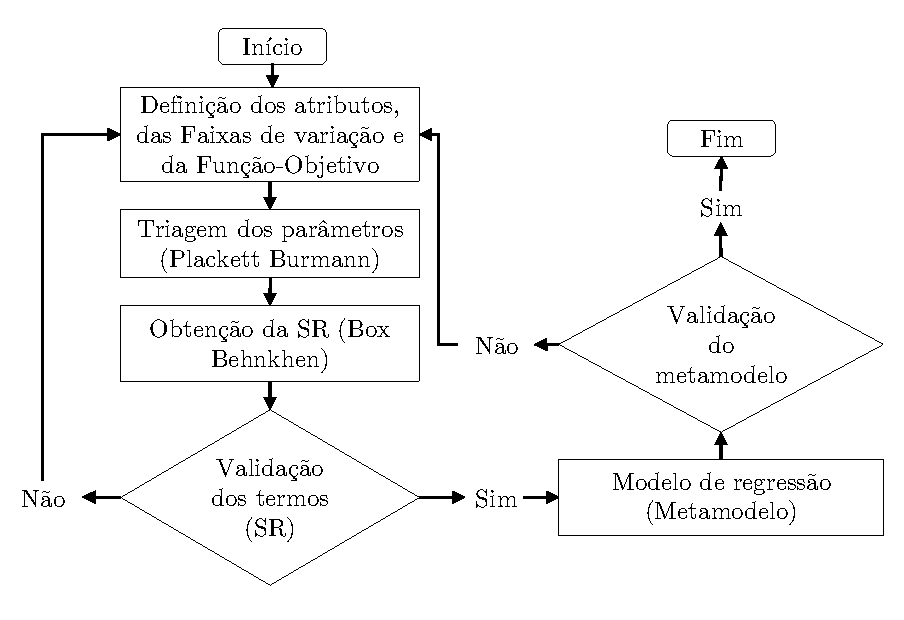
\includegraphics{Figuras/suprespostametodologia.pdf}  
    \caption{Metodologia de Planejamento estatístico.}  
    \legend{Fonte: Adaptado de \citeonline{lemma}}
}
    \label{fig:planestatistico}  
\end{figure}


Na etapa inicial, foi necessário definir os atributos incertos, estabelecer sua faixa de valores e determinar a distribuição de probabilidade das variáveis que poderiam influenciar as previsões da taxa de erosão, de acordo com o estudo bibliográfico. Nessa etapa, os atributos foram padronizados em três níveis incertos, conforme descrito na etapa de discretização das variáveis aleatórias em níveis de probabilidades (capítulo \ref{cap:Variáveis aleatórias e distribuições de probabilidades}).

 Neste trabalho, para a etapa de triagem dos atributos, as simulações numéricas foram realizadas conforme um planejamento experimental fatorial fracionado do tipo Plackett–Burman, com objetivo de comparar os resultados com a Análise de sensibilidade. Esta aplicação é adequada para realizar uma análise superficial na fase inicial de estudo, uma vez que requer poucos experimentos. Foram estudadas estatisticamente a influência de 7 atributos na taxa erosiva:  Tamanho do cascalho, Forma do cascalho, Densidade do cascalho, Densidade do fluido de perfuração, Viscosidade do fluido de perfuração, Velocidade de escoamento e Vazão mássica. A Tabela \ref{tab:box4} apresenta a matriz do planejamento utilizado nesta etapa e os respectivos valores das variáveis aleatórias estudadas.

\begin{table}[H] 
\caption{Matriz do planejamento Plackett Burmann para 7 variáveis de entrada.}
\begin{tabular*}{\textwidth}{@{\extracolsep{\stretch{1}}}*{8}{c}@{}}
\toprule
   Simulação &VM&	DC	&TAM	&VEL&	FM&	DF	&VISC\\
  \midrule
01 & 0.13 &	2350 &	0.24	& 8.87   &	0.49 &	1250 &	15 	\\
02 & 0.13 &	2950 &	0.86	& 8.87  &	0.87 &	1250 &	15 	\\
03 & 0.27 &	2350 &	0.24	& 8.87  &	0.87 &	1500 &	35   \\
04 & 0.13 &	2950&	0.24	& 8.87   &	0.49 &	1500 &	35    \\
05 & 0.13 &	2950 &	0.86	& 10.13  &	0.49 &	1500 &	35     \\
06 & 0.27 &	2950 &	0.24	& 10.13	 &  0.87 &	1250 &	35     \\
07 & 0.27 &	2350 &	0.86	& 10.13	 &  0.49 &	1500 &	15 	\\
08 & 0.13 &	2350 &	0.86	& 10.13 &  0.87 &	1250 &	35 	\\
09 & 0.13 &	2350 &	0.24	& 10.13	 &  0.87 &	1500&	15 	\\
10 & 0.27 &	2350 &	0.86	& 8.87	 &  0.49 &	1250&	35 	\\
11 & 0.27 &	2950 &	0.86	& 8.87	 &  0.87 &	1500&	15 	\\
12 & 0.27 &	2950 &	0.24    & 10.13	 &  0.49 &	1250 &	15	\\

\bottomrule   
\end{tabular*}
\label{tab:box4}
\subcaption{VM: Vazão massica(kg/s); VISC: Viscosidade do fluido de perfuração(cP); TAM: Tamanho(mm); VEL: Velocidade de escoamento(m/s).}
\legend {Fonte: o autor.}
\label {tab:placket7var}
\end{table}

Na segunda etapa, o objetivo foi identificar os parâmetros que possuem um impacto significativo na função objetivo. Isso foi feito por meio da análise de variância (ANOVA), a fim de determinar a melhor maneira de conduzir estudos adicionais, como a construção da superfície de resposta e a análise de risco, com o menor custo computacional possível.

Após a realização da análise de variância do planejamento de Plackett-Burman proposto e a análise de sensibilidade, foram selecionadas as variáveis mais significativas em relação ao desgaste erosivo. Essas variáveis foram utilizadas na elaboração da matriz de experimentos de Box-Behnken, que é uma técnica de planejamento experimental que permite explorar de forma eficiente a região de interesse e obter informações sobre as interações entre as variáveis.

Para a obtenção da Superfície de resposta (SR), foi realizada a combinação dos termos definidos em uma matriz de ensaio experimental definida pelo planejamento estatístico de Box Benhkhen. O número total de simulações realizadas para a matriz de Box Behkehn é \textit{N = 2 * k * (k − 1) + Co}, em que \textit{k} é o número de atributos e \textit{Co} é o número de pontos centrais. A Tabela \ref{tab:box5555} apresenta a matriz codificada do planejamento utilizado nesta etapa e os respectivos valores das variáveis. As variáveis presentes nos ensaios computacionais, foram definidas na etapa de triagem de atributos por análise de sensibilidade e significância estatística dos termos por Plackett Burmann, que seráão detalhadas nos resultados do capítulo \ref{sec:Seleçãodosatributoscríticos} .

\begin{table}[H]
\caption{Matriz do planejamento Box Benhkhen para 4 variáveis de entrada.}
\begin{tabular*}{\textwidth}{@{\extracolsep{\stretch{1}}}*{5}{c}@{}}
 \toprule
   Simulação &VM	&VISC	&TAM	&VEL	\\
  \midrule

1         & 0.13 & 15   & 0.55 & 9.50  \\
2         & 0.27 & 15   & 0.55 & 9.50  \\
3         & 0.13 & 35   & 0.55 & 9.50  \\
4                                 & 0.27                         & 35   & 0.55 & 9.50  \\
5                                 & 0.20                         & 25   & 0.24 & 8.87  \\
6                                 & 0.20                         & 25   & 0.86 & 8.87  \\
7                                 & 0.20                         & 25   & 0.24 & 10.13 \\
8                                 & 0.20                         & 25   & 0.86 & 10.13 \\
9                                 & 0.13                         & 25   & 0.55 & 8.87  \\
10                                & 0.27                         & 25   & 0.55 & 8.87  \\
11                                & 0.13                         & 25   & 0.55 & 10.13 \\
12                                & 0.27                         & 25   & 0.55 & 10.13 \\
13                                & 0.20                         & 15   & 0.24 & 9.50  \\
14                                & 0.20                         & 35   & 0.24 & 9.50  \\
15                                & 0.20                         & 15   & 0.86 & 9.50  \\
16                                & 0.20                         & 35   & 0.86 & 9.50  \\
17                                & 0.13                         & 25   & 0.24 & 9.50  \\
18                                & 0.27                         & 25   & 0.24 & 9.50  \\
19                                & 0.13                         & 25   & 0.86 & 9.50  \\
20                                & 0.27                         & 25   & 0.86 & 9.50  \\
21                                & 0.20                         & 15   & 0.55 & 8.87  \\
22                                & 0.20                         & 35   & 0.55 & 8.87  \\
23                                & 0.20                         & 15   & 0.55 & 10.13 \\
24                                & 0.20                         & 35   & 0.55 & 10.13 \\
25                                & 0.20                         & 25   & 0.55 & 9.5  \\

\bottomrule 
\end{tabular*}
\label{tab:box5555}
\subcaption{VM: Vazão massica(kg/s); VISC: Viscosidade do fluido de perfuração(cP); TAM: Tamanho(mm); VEL: Velocidade de escoamento(m/s).}
\legend {Fonte: o autor.}
\end{table}



A análise estatística do planejamento de Box Benhkhen foi realizada através da aplicação da Análise de Variância (ANOVA) aos termos da Superfície de Resposta, avaliando o p-valor e Teste F dos termos lineares, de interação e quadráticos. Foi estimada a precisão adequada do modelo para verificar a relação entre sinal-ruído, comparando o range de valores previstos pelo modelo nos pontos de ensaios da matriz de experimentos com o erro médio de previsão. 

Com a estrutura de dados adquirida e validada estatisticamente, foi obtida a equação matemática com os termos significativos que descreve a resposta da superfície. Em seguida, os valores simulados de desgaste erosivo utilizados para construir a resposta da superfície foram comparados com os valores obtidos de desgaste erosivo pela equação de regressão do modelo, a fim de realizar o teste de consistência, ou seja, verificar se o modelo está prevendo adequadamente os dados de simulação numérica. A validação cruzada foi realizada comparando os valores obtidos pela simulação com os valores previstos pelo modelo de regressão. Os coeficientes de determinação R², R² ajustado e R² predito foram utilizados para avaliar a qualidade do modelo. Se os termos do modelo não forem estatisticamente validados ou se a validação cruzada não apresentar um bom coeficiente de determinação, as etapas da metodologia devem ser refeitas. Ao passo que o metamodelo de regressão passar pela verificação de validação estatística e que não apresente caracteristicas consideravelmente divergentes da simulação numérica CFD, ele pode ser aplicado para prever novos cenários de erosão. Neste trabalho, o metamodelo foi utilizado para gerar curvas de risco para a função-objetivo de erosão de \citeonline{oka} nos processos de análise que envolvem muitos cenários de simulação (Monte Carlo e Árvore de derivação). 

A validação das respostas dos modelo gerados pelos planejamentos de experimentos de Plackett-Burmann e Box Benhkhen requer a aplicação de testes estatísticos recomendados por \cite{montgomery}. Esses testes são essenciais para avaliar a adequação do modelo aos dados. Uma das etapas dessa validação envolve a análise da normalidade dos resíduos do modelo. Com este objetivo, foi utilizado o gráfico de probabilidade normal com objetivo comparar a função de distribuição acumulada empírica (ECDF) dos resíduos com a distribuição esperada para resíduos com comportamento normal. Também foi aplicado o teste de hipóteses de Kolmogorov-Smirnoff que consiste em uma técnica estatística não paramétrica que é usada para verificar se existem evidências de normalidade dos resíduos. Além disso, foi de suma importância verificar a constância da variância dos resíduos, ou seja, se eles apresentavam evidências de homocedasticidade. A suposição de homocedasticidade era fundamental para a análise de regressão do modelo ajustado. Caso os resíduos demonstrassem uma dispersão constante em relação aos valores preditos, validava-se a suposição de homocedasticidade.


\section{Análise de Risco por Árvore de Derivação}

A composição da Árvore de Derivação foi realizada a partir dos resultados da análise de sensibilidade e de Plackett Burmann, ou seja, somente os atributos críticos (z) e seus respectivos níveis de incerteza (y) foram utilizados para combinação para obtenção da curva de risco. O número de ramificações, ou seja, a quantidade de combinações presentes na Árvore de derivação é representada por $y^z$ = modelos de simulação. Deste modo, a partir da definição dos atributos críticos foram gerados 81 cenários de simulação para composição da Árvore de derivação. Após simulação fludidinâmica dos cenários determinados, os dados foram tratados estatisticamente para obtenção da curva de risco de falha por erosão.


\section{Análise de risco por Monte Carlo}


Uma etapa de análise de risco realizada neste trabalho, é o emprego da técnica de
Monte Carlo para a combinação dos atributos críticos e obtenção da curva de risco de falha por erosão. A Figura \ref{fig:montecarloflux} demonstra as etapas realizadas para a composição dos cenários de simulação de Monte Carlo.

\begin{figure}[H] 
    \centering  
    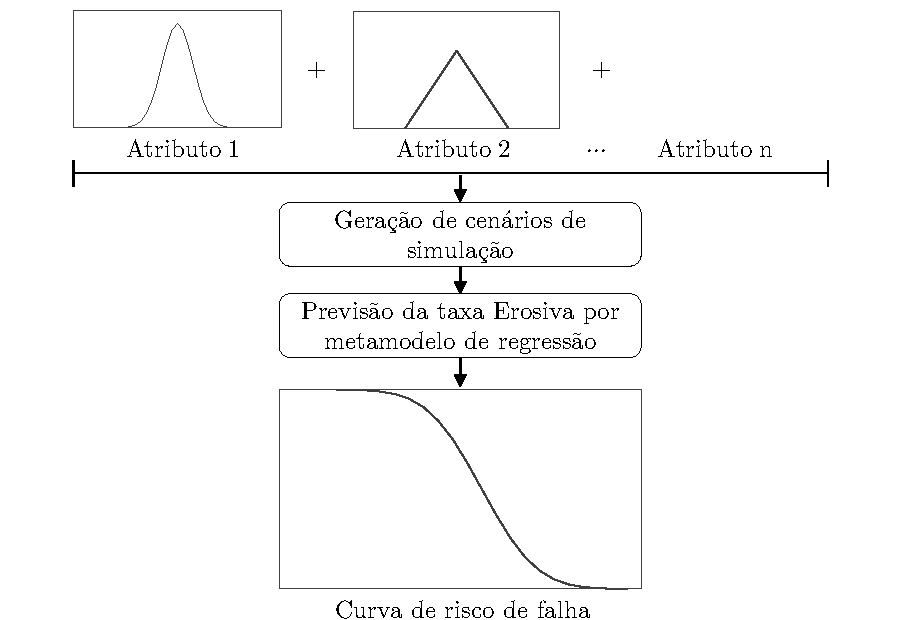
\includegraphics{Figuras/metodologiaMC.pdf}  
    \caption{Metodologia de Monte Carlo para Análise de risco de falha por erosão.}  
    \legend{Fonte: o autor.}
    \label{fig:montecarloflux}  
\end{figure}

Na primeira etapa, foram realizadas amostragens aleatórias nos atributos que exercem influência sobre a taxa erosiva de Oka, determinados no planejamento estatístico de Plackett Burmann. Os valores foram amostrados de acordo com a distribuição de probabilidade de cada variável. Assim, os atributos foram combinados para gerar um número elevado de cenários e produzir uma estimativa consistente da função de distribuição de probabilidade para a resposta de erosão do modelo de Oka. Para estimar o número de cenários ideal para o método de Monte Carlo, foi utilizado o cálculo do coeficiente de variação (CoV), que é um indicador de flutuação em torno da média de uma variável aleatória. O Cov é um parâmetro adimensional, dado por:

\begin{equation}
    CoV (\%) =  \frac{\sigma X}{\mu X}
\end{equation}

Na qual:

$\sigma$X= Média amostral;

$\mu$X= Desvio padrão amostral.

\vspace{0.3cm}

O número de cenários ideal para os sorteios de Monte Carlo foi definido a partir da estabilização do coeficiente de variação (Cov), obtido pelos diferentes cenários realizados pelo método de Monte Carlo. Devido ao elevado número de cenários, para previsão da resposta de erosão de Oka, foi utilizado o metamodelo de regressão gerado pelo planejamento de Superfície de resposta. A partir das respostas dos cenários, foi possível obter as curvas de risco. Nessa etapa, foram plotadas curvas geradas com diferentes números de sorteios, a fim de avaliar a influência da quantidade de cenários nas respostas do método de Monte Carlo e comparar com a curva de risco gerada pelo método de Árvore de derivação.











\chapter{Resultados}

\section{Modelo de simulação fluidodinâmica computacional}


No contexto de um fluxo específico, a ocorrência de dano erosivo é observada em várias áreas das paredes da tubulação, devido às colisões de cascalhos em várias regiões durante o escoamento, sob diferentes condições. Contudo, embora existam diferentes magnitudes de taxa erosiva, numa mesma condição de fluxo e para um mesmo material, o que de fato interessa para a análise de risco, é o ponto da tubulação onde ocorre a maior taxa erosiva, ou seja, a região onde o material irá falhar primeiro. Deste modo, a taxa erosiva máxima é a função-objetivo de análise deste trabalho em todos os cenários de simulação de fluxo estacionários realizados. Conforme demonstrado na Figura \ref{fig:maiorerosao}, para este exemplo de simulação fluidodinâmica, o valor máximo de erosão foi de aproximadamente 8E-08 kg/m.s² ocorrendo num ângulo de aproximadamente 70° da curva. 

\begin{figure}[H] 
    \centering  
    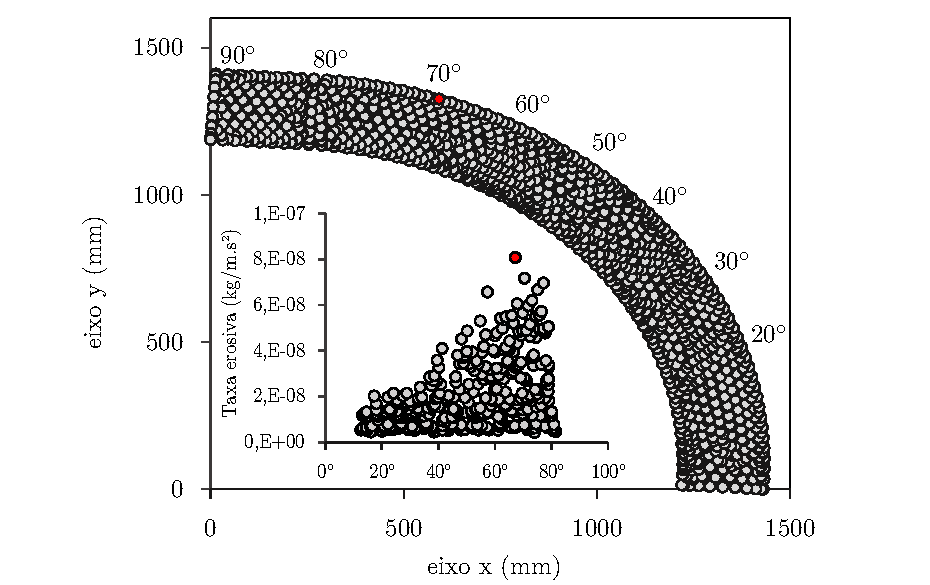
\includegraphics[width=0.85\textwidth]{Figuras/pontodemaiiorerosao.pdf}  
    \caption{Ponto de maior erosão resultante da simulação fluidodinâmica computacional.}  
    \legend{Fonte: o autor.}
    \label{fig:maiorerosao}  
\end{figure}

O modelo de \citeonline{oka} aplicado em simulações computacionais CFD, foi comparado e validado com base em ensaios experimentais em curvas de 90º de raio curto \cite{liuuh}, a mesma geometria utilizada no presente trabalho (Figura \ref{fig:cfdgeometria}). Portanto, as taxas de erosão foram obtidas utilizando o modelo proposto por \citeonline{oka} matematicamente formulado na Equação \ref{equationoka}. Este modelo foi relacionado interativamente com as equações de transporte do fluido e das partículas, de modo que ao final fosse possível obter as taxas de erosão ao longo de toda parede do duto.

A convergência do modelo fluidodinâmico foi analisada verificando os resíduos das equações governantes do modelo (Figura \ref{fig:cfdcontinuidade}). Embora haja baixos valores residuais e um comportamento de convergência das equações governantes, é possível que a solução física de escoamento não convirja. Desse modo, como alternativa complementar para análise do modelo, foi monitorado a convergência física do parâmetro de velocidade de escoamento na saída do fluido do sistema (Figura \ref{fig:cfdcontinuidade2}).

\begin{figure}[H] 
    \centering  
    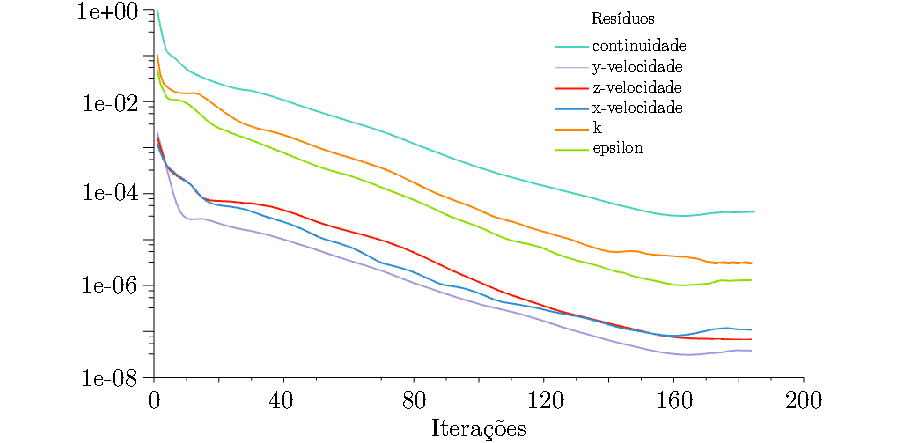
\includegraphics[width=0.90\textwidth]{Figuras/cfddecontinuidade.pdf}  
    \caption{Convergência dos resíduos do modelo fluidodinâmico.}  
    \legend{Fonte: o autor.}
    \label{fig:cfdcontinuidade}  
\end{figure}


\begin{figure}[H] 
    \centering  
    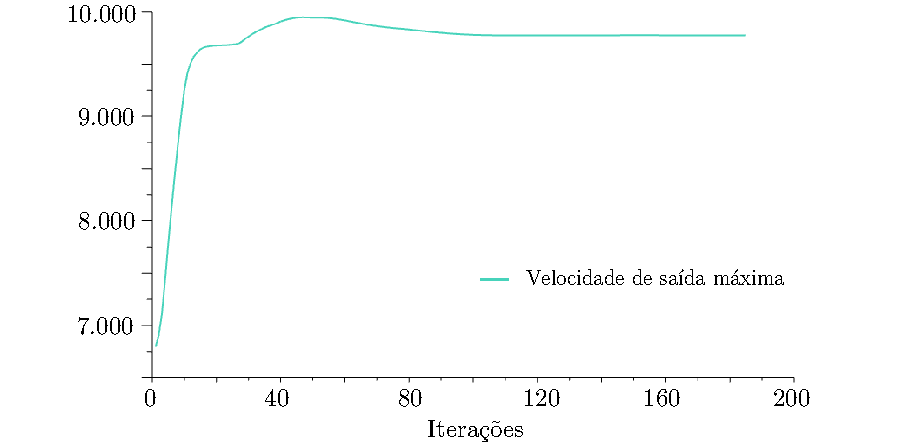
\includegraphics[width=0.90\textwidth]{Figuras/cfddecontinuidade2.pdf}  
    \caption{Convergência da velocidade de escoamento na saída do fluido do sistema.}  
    \legend{Fonte: o autor.}
    \label{fig:cfdcontinuidade2}  
\end{figure}

A convergência do modelo foi obtida com aproximadamente 180 iterações, conforme ilustra a Figura \ref{fig:cfdcontinuidade}. Embora seja possível visualizar uma
convergência a partir de 110 iterações para a velocidade média do escoamento na saída do sistema, como pode ser visualizado pelo gráfico da Figura \ref{fig:cfdcontinuidade2}. Assim, é possível inferir que houve convergência física do modelo durante todo o domínio físico, através da resolução de equações de fenômenos de transporte que caracterizam o escoamento de fluidos e validar a utilização do modelo de fluxo para obtenção do desgaste erosivo para este estudo. 

\section{Seleção dos atributos críticos}
\label{sec:Seleçãodosatributoscríticos} 

Antes de se realizar o planejamento de experimentos para obtenção da Superfície de reposta, é necessário um estudo prévio da influência dos atributos na função-objetivo de interesse. Para o caso em estudo, na análise de sensibilidade foram necessárias 15 simulações para realizar a variação de um atributo por vez, a partir do caso base em que as variáveis foram fixadas no nível intermediário (0). A Figura \ref{fig:efeitossensi} demonstra um gráfico do tipo tornado com os efeitos percentuais dos atributos na resposta de desgaste erosivo, o que permite observar se a mudança de nível (-1)
para (+1) de uma determinada variável resulta em aumento ou diminuição da taxa
erosiva, bem como os atributos que exercem maior impacto na resposta. 

\begin{figure}[H] 
    \centering  
    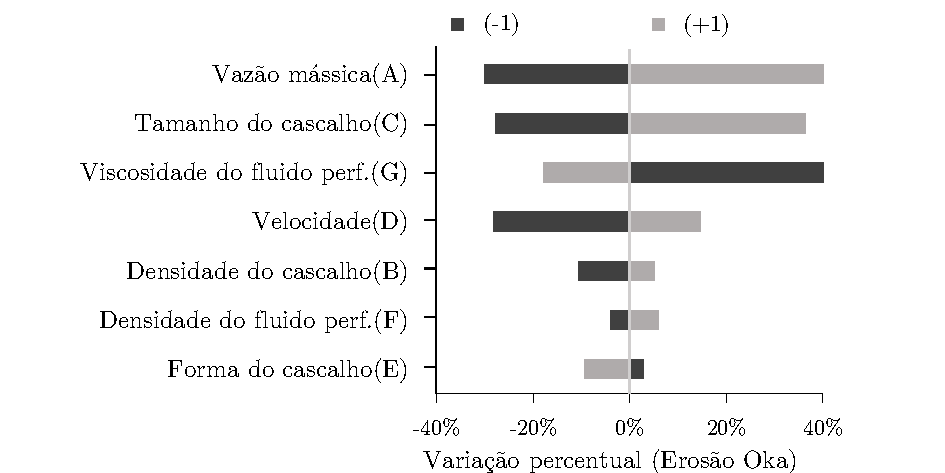
\includegraphics{Figuras/analisesensi.pdf}  
    \caption{Gráfico de efeitos percentuais dos atributos no desgaste erosivo.}  
    \legend{Fonte: o autor.}
    \label{fig:efeitossensi}  
\end{figure}

Os atributos incertos: "Forma do cascalho" e a "Viscosidade do fluido de perfuração", foram investigados em relação à taxa erosiva. Os valores desses atributos foram estudados em dois níveis, -1 e +1. Observou-se que o aumento dessas variáveis resultou em uma diminuição na taxa erosiva. Esses resultados físicos estão em concordância com estudos anteriores \cite{yabuki}, \cite{walker}, \cite{hutchings}. Dentro das faixas de estudo consideradas, foi observado que as variáveis de "Vazão mássica", "Tamanho do cascalho", "Velocidade", "Densidade do cascalho" e "Densidade do fluido de perfuração" apresentaram um aumento no desgaste erosivo ao serem incrementadas do nível (-1) para o nível (+1). Esses resultados estão em conformidade com os trabalhos anteriores \cite{clark}, \cite{albu},\cite{kowsari}, \cite{kumar}, \cite{hutchings}, \cite{ANUR}. É possível verificar, que os atributos que mais influenciam taxa erosiva dentro das faixas estudadas das variáveis aleatórias foram, respectivamente, "Vazão mássica", "Tamanho do cascalho", "Viscosidade do fluido de perfuração" e "Velocidade". A "densidade do cascalho" e do "Fluido de perfuração" e a "Forma dos cascalhos" exerceram pouco impacto na resposta de erosão comparados aos demais atributos para as faixas estudadas de variação.

O método do planejamento estatístico de Plackett Burmann foi empregado nesta etapa também com a finalidade de realizar uma triagem dos atributos que mais influenciam na taxa desgaste erosivo de Oka. Na Tabela \ref{tab:anovaplack} são apresentadas as análises dos efeitos em relação aos atributos puros, deste modo é possível definir quais variáveis têm maior impacto sobre a função-objetivo, que por sua vez, foi obtida através da seleção do ponto da tubulação em que o valor de desgaste é mais severo nos diversos cenários de fluxo simulados, conforme demonstrado na Figura \ref{fig:maiorerosao}. A Tabela \ref{tab:anovaplack} apresenta a Análise de variância com os resultados da análise estatística obtidos pelo Planejamento de Plackett Burmann, apresentando as Somas de quadrados (SQ), Graus de liberdade (GL), Médias quadráticas (MQ) e valores dos testes estatísticos F e p associados a cada fonte de variação do estudo de Desgaste Erosivo. Essas fontes de variação incluem os fatores de interesse, como diferentes tratamentos ou grupos experimentais computacionais, além de possíveis fatores de confusão ou erros.


\begin{table}[!h]
\caption{Análise de variância para o planejamento Plackett-Burman.}
\begin{tabular*}{\textwidth}{@{\extracolsep{\stretch{1}}}*{6}{c}@{}}
 \toprule
Fonte & GL & SQ Aj. & MQ Aj. & Valor F & Valor-P \\
  \midrule

   
        Modelo* & 7 & 2.10E-09 & 2.99E-10 & 19.20 & 0.006 \\ 
        Linear* & 7 & 2.10E-09 & 2.99E-10 & 19.20 & 0.006 \\ 
        Vazão mássica* & 1 & 7.50E-10 & 7.49E-10 & 47.97 & 0.002 \\ 
        Densidade do cascalho & 1 & 1.00E-11 & 5.40E-12 & 0.34 & 0.589 \\ 
        Tamanho* & 1 & 6.50E-10 & 6.51E-10 & 41.70 & 0.003 \\ 
        Velocidade* & 1 & 2.10E-10 & 2.11E-10 & 13.55 & 0.021 \\ 
        Forma & 1 & 2.00E-11 & 2.48E-11 & 1.59 & 0.276 \\ 
        Densidade do fluido de perfuração & 1 & 4.00E-11 & 4.28E-11 & 2.74 & 0.173 \\ 
        Viscosidade* & 1 & 4.10E-10 & 4.13E-10 & 26.48 & 0.007 \\ 
        Erro & 4 & 6.00E-11 & 1.56E-11 & ~ & ~ \\ \
        Total & 11 & 2.16E-09 \\ 

\bottomrule   
\end{tabular*}
\label{tab:anovaplack}
\subcaption{* Termos estatisticamente significativos com intervalo de 95\% de confiança.}
\legend {Fonte: o autor.}
\end{table*}
\end{table}

A partir da análise da tabela de ANOVA, foram obtidas informações para a interpretação dos resultados do estudo. A tabela permitiu identificar os atributos que apresentam uma diferença significativa entre os grupos ou tratamentos analisados, indicando os fatores independentes que possuem um efeito estatisticamente relevante na variável dependente. A partir da análise das medidas de variabilidade, como os quadrados médios e os valores F associados aos Graus de Liberdade, foi utilizado o teste estatístico de Fischer para determinar a significância estatística do modelo obtido (Figura \ref{fig:fischerplackett}).

\begin{figure}[H] 
    \centering  
    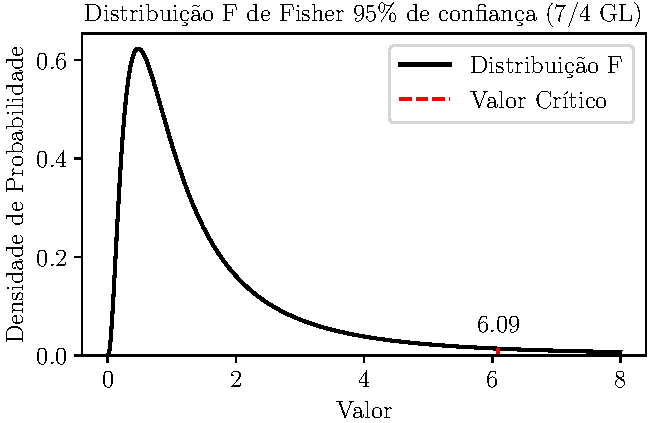
\includegraphics{Figuras/fischerplackett.pdf}  
    \caption{Distribuição de Fischer para análise de significância.}  
    \legend{Fonte: o autor.}
    \label{fig:fischerplackett}  
\end{figure}


A fonte de variação do "Modelo" refere-se ao modelo global utilizado na análise de variância. Conforme observado pela Figura \ref{fig:fischerplackett}, a distrubuição de Fischer para o modelo associado aos Graus de liberdade (7/4), indica um F crítico de 6.09 para um nível de significância de 95\%, o valor F calculado do modelo 19.20 indica que há uma diferença significativa entre os grupos ou tratamentos considerados neste estudo (com um valor-p associado de 0.006). Isso significa que as variáveis independentes têm um efeito estatisticamente relevante na variável dependente. Foram efetuados os cálculos de F para todos os termos com seus respectivos Graus de Liberdade o que determinou os Atributos com significância estatística. As variáveis: "Vazão mássica", "Tamanho do cascalho", "Velocidade" e "Viscosidade do fluido" apresentaram valores F significativos, indicando que elas têm um impacto estatisticamente significativo no Desgaste Erosivo.

A Figura \ref{fig:efeitosplackett} analisa os efeitos principais dos atributos em relação ao desgaste erosivo, o que permite observar se a mudança de nível (-1) para (+1) de uma determinada variável resulta em aumento ou diminuição da taxa erosiva. 





\begin{figure}[H] 
    \centering  
    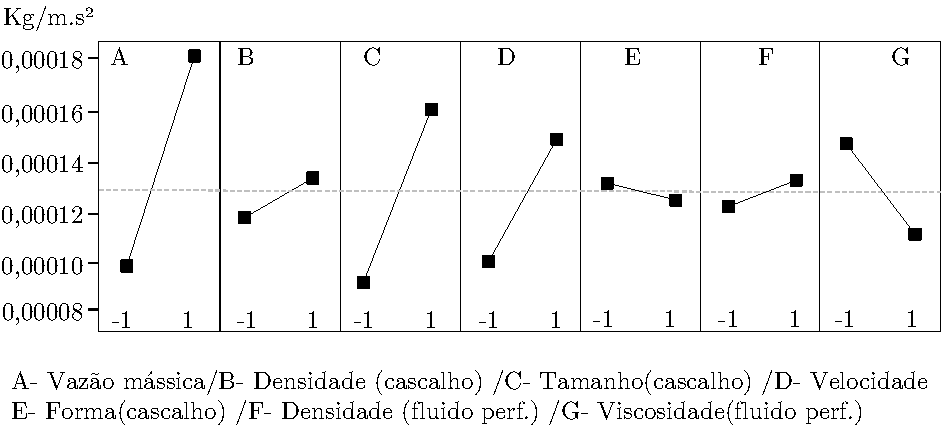
\includegraphics{Figuras/efeitosPLACKETT.pdf}  
    \caption{Gráfico de efeitos principais com médias ajustadas para o Desgaste erosivo.}  
    \legend{Fonte: o autor.}
    \label{fig:efeitosplackett}  
\end{figure}

Dentro das faixas de estudo consideradas, verificou-se que os atributos incertos "Forma" e "Viscosidade" apresentaram uma diminuição na taxa erosiva quando houve a mudança de nível de (-1) para (+1). Isso indica que o aumento dessas variáveis resulta em uma redução no desgaste erosivo. Por outro lado, observou-se que as variáveis "Vazão mássica", "Tamanho do cascalho", "Velocidade", "Densidade do cascalho" e "Densidade do fluido de perfuração" apresentaram um aumento no desgaste erosivo ao serem incrementadas do nível -1 para o nível +1. Esses resultados estão em conformidade com estudos anteriores que também relataram essas relações entre as variáveis e o Desgaste erosivo \cite{yabuki}, \cite{walker}, \cite{hutchings},\cite{clark}, \cite{albu},\cite{kowsari}, \cite{kumar}, \cite{hutchings}, \cite{ANUR}. A Figura \ref{fig:paretoplackett} apresenta o gráficos de Pareto dos efeitos principais para a resposta da taxa Desgaste erosivo de Oka. Este gráfico exibe de forma rápida e objetiva os efeitos que foram estatisticamente significativos com 95 \% de nível de significância, ou seja, os que apresentam valores resultantes maiores que a linha tracejada em vermelho.

\begin{figure}[H] 
    \centering  
    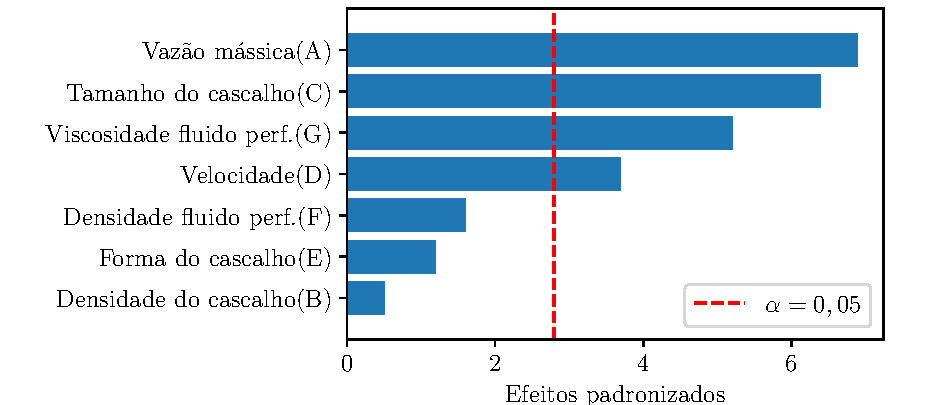
\includegraphics{Figuras/PLACKETTBURMANNNN.pdf}  
    \caption{Gráfico de pareto dos efeitos padronizados.}  
    \legend{Fonte: o autor.}
    \label{fig:paretoplackett}  
\end{figure}

Observando os resultados da Tabela \ref{tab:anovaplack} e Figura \ref{fig:paretoplackett}, os atributos "Forma do cascalho", "Densidade do fluido perfuração" e "Densidade do cascalho", não exerceram impacto significativo sobre o Desgaste erosivo, uma vez que seus respectivos valores F foram menores que os valores críticos para o intervalo de confiança de 95\%. Para validar as resposta do modelo gerado por Plackett Burmann foi necessária a realização de testes estatísticos recomendados por \citeonline{montgomery}. Para tanto, foram gerados os gráficos de probabilidade normal e análise de homocedasticidade dos resíduos (Figuras \ref{fig:probnormalplackett} e \ref{fig:residuosplackett}).

\begin{figure}[H] 
    \centering  
    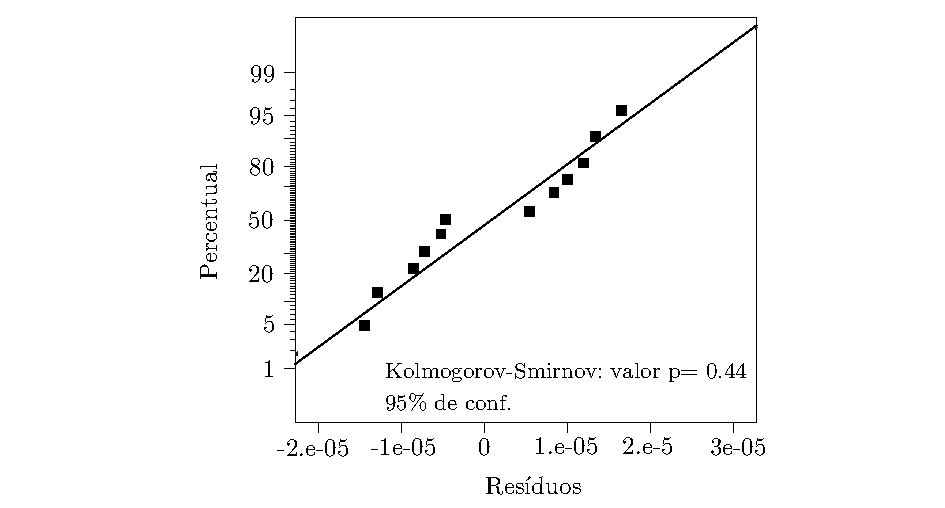
\includegraphics[width=0.92\textwidth]{Figuras/probnormalplacket.pdf}  
    \caption{Gráfico de probabilidade normal.}  
    \legend{Fonte: o autor.}
    \label{fig:probnormalplackett}  
\end{figure}


\begin{figure}[H] 
    \centering  
    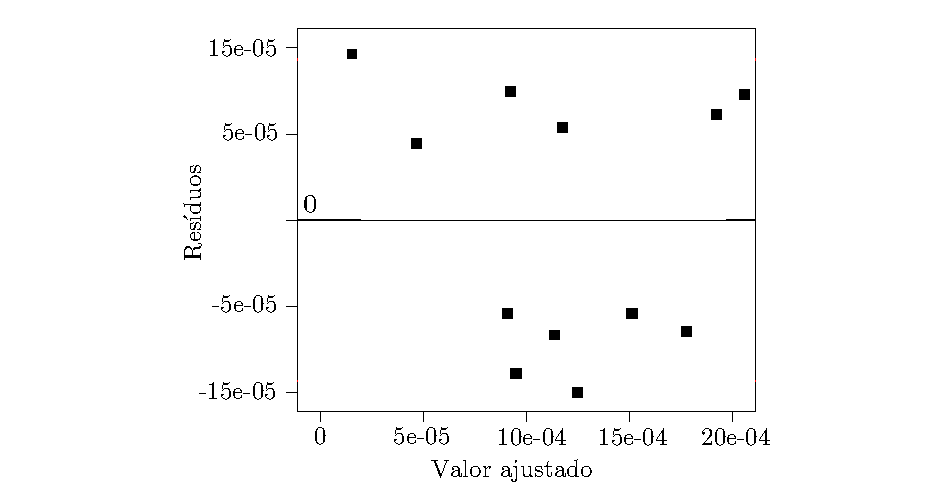
\includegraphics[width=0.92\textwidth]{Figuras/residuosPLACKETT.pdf}  
    \caption{Gráfico de resíduos versus Valores ajustados.}  
    \legend{Fonte: o autor.}
    \label{fig:residuosplackett}  
\end{figure}

Deste modo, através da análise das Figuras \ref{fig:probnormalplackett} e \ref{fig:residuosplackett} é possível verificar que os resíduos apresentam distribuição normal e homocedasticidade, ou seja, aleatoriedade em torno de um valor médio. Para validar esta hipótese, foi realizado o teste de normalidade de Kolmogorov-Smirnov. Para o ensaio de Plackett-Burmann realizado, o valor p do teste Kolmogorov-Smirnov foi de 0.44, o que indica que os resíduos seguem uma distribuição normal. Os métodos de Análise de sensibilidade e planejamento fatorial Plackett Burmann apresentaram respostas semelhantes em termos dos atributos críticos. Os parâmetros: "Vazão mássica", "Tamanho do cascalho", "Viscosidade fluido perfuração" e "Velocidade" evidenciaram significância estatística para a função-objetivo. Consequentemente, essas variáveis serão incorporadas na geração dos metamodelos de regressão por Superfície de Resposta e utilizadas na obtenção das curvas de risco. Por outro lado, os demais atributos foram mantidos no nível mais provável (0) em todas as etapas posteriores, resultando em uma redução no número de simulações numéricas necessárias nas etapas de Superfície de Resposta e Análise de Risco. Essa redução contribui para uma diminuição do tempo computacional necessário para realizar tais análises.


\section{Planejamento estatístico (Superfície de resposta)}

Na seção \ref{sec:Planejamentoestatistico}, o Planejamento fatorial fracionário Plackett Burmann foi utilizado para realizar a triagem dos atributos incertos de perfuração de poços, ou seja, para selecionar as variáveis mais significativas para o processo de Análise de risco. Nesta etapa, o planejamento de experimentos é aplicado para encontrar a Superfície de resposta, ou seja, a equação de regressão que irá compor o metamodelo para substituição das simulações computacionais no processo de Análise de risco. Os fatores estudados neste planejamento foram restringidos aos quatro identificados como significativos no planejamento de Plackett Burmann, sendo eles: "Vazão mássica(A)", "Tamanho do cascalho(C)", "Viscosidade fluido perf.(G)" e "Velocidade(D)". Deste modo, a matriz de planejamento criada foi composta por 25 pontos, sendo 1 ponto central, o que representa 25 modelos para serem simulados por fluidodinâmica computacional. De posse de todos os modelos simulados, foi realizada uma regressão multivariada, e foram obtidos os termos da Superfície de Resposta estatísticamente significativos através da Análise de Variância (Tabela \ref{tab:anovabox}).

\begin{table}[!h]
\caption{Análise de variância do modelo de regressão (Superfície de resposta).}
\begin{tabular*}{\textwidth}{@{\extracolsep{\stretch{1}}}*{6}{c}@{}}
 \toprule
  Fonte&SQ (Aj.)&	GL	&QM (Aj.)&	Valor F& Valor P\\
  \midrule

Modelo(Regressão)*&	1.87E-09&	8&	2.34E-10&	53.91&	< 0.0001\\
Vazão mássica*&	6.59E-10&	1&	6.59E-10&	151.85&	< 0.0001\\
Viscosidade*&	1.81E-10&	1&	1.81E-10&	41.68&	< 0.0001\\
Tamanho*&	6.32E-10&	1&	6.32E-10&	145.44&	< 0.0001\\
Velocidade*&3.07E-10&	1&	3.07E-10&	70.72&	< 0.0001\\
Vazão mássica x Viscosidade* &	1.52E-11&	1&	1.52E-08&	3.50&	0.0497\\
Tamanho x Velocidade*&	1.98E-11&	1&	1.98E-08&	4.56	&0.0485\\
Vazão mássica²*&	2.25E-11&	1&	2.25E-11&	5.18&	0.0370\\
Tamanho²*&	5.05E-11&	1&	5.05E-11&	11.64&	0.0036\\
Resíduo&	6.95E-11&	16	&4.34E-12	\\	
Total&	1.94E-09&	24	\\		

  \bottomrule   
\end{tabular*}
\label{tab:anovabox}
\subcaption{* Termos estatisticamente significativos com intervalo de 95\% de confiança.}
\legend {Fonte: o autor.}
\end{table*}
\end{table}

A tabela de Análise de Variância foi empregada para examinar os resultados do estudo e identificar os atributos que demonstram diferenças estatisticamente significativas entre os grupos ou tratamentos analisados. Essa análise possibilitou determinar quais fatores independentes apresentam um efeito estatisticamente relevante na variável dependente, por se tratar de um estudo de Superfície de Resposta através do planejamento estatístico de Box Behnkhen, é possível verificar além dos termos lineares, os termos de interação e quadráticos. Para isso, foram consideradas medidas de variabilidade, como os quadrados médios e os valores F associados aos Graus de Liberdade. O teste estatístico de Fischer foi utilizado para verificar a significância estatística do modelo obtido. Essa abordagem permitiu uma interpretação dos resultados, destacando os fatores que exercem influência estatisticamente relevante no desgaste erosivo.


\begin{figure}[H] 
    \centering  
    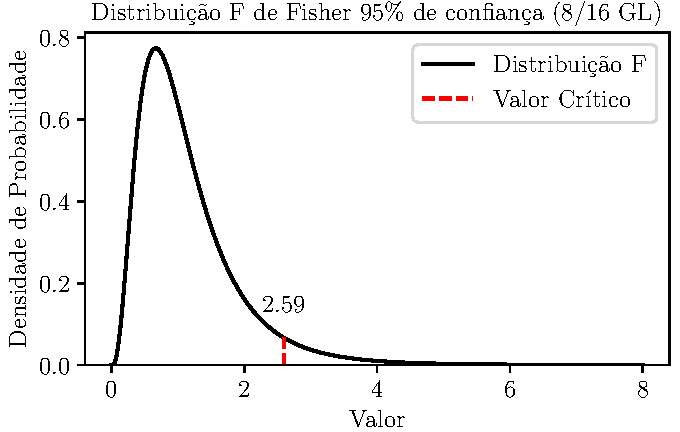
\includegraphics{Figuras/fischerbox.pdf}  
    \caption{Distribuição de Fischer para análise de significância.}  
    \legend{Fonte: o autor.}
    \label{fig:fischerbox}  
\end{figure}


Através da análise de Figura \ref{fig:fischerbox}, é possível verificar que o Modelo de Regressão gerado a partir do planejamento de Box Benhkhen é válido estatisticamente. O valor de F calculado (53.91) do modelo, levando em consideração o número de graus de liberdade do planejamento, é superior ao F crítico (2.59) para 95\% de nível de significância. Foram efetuados os cálculos
de F para todos os termos com seus respectivos Graus de Liberdade o que determinou os atributos com significância estatística para o modelo. A partir da validação estatística do modelo de regressão incluindo os termos lineares, quadráticos e de interação significativos, foi possível gerar a equação com os coeficientes dos termos para a previsão do desgaste de Erosão de Oka, que constitui o metamodelo (Equação \ref{eq:metamodelo}). 
 

\begin{equation}
\begin{align*} 
E = -5.4435x10^{-5} + 0.0003(A) + 1.6880x10^{-7}(G) - 0.0508(C) + 1.7630x10^{-6}(D)\\ 
- 2.7877x10^{-6}(A)(G) + 0.0114(C)(D) - 0.0004(A)^2 - 30.8644(C)^2 \quad \quad \quad \;  \, \, \, \, \, \, \,\, \\ 
\end{align*}
\label{eq:metamodelo}
\end{equation}

Onde:

E = é a taxa de erosão (kg/m.s²);

A= Vazão mássica (kg/s);

C= Tamanho do cascalho(mm);

D= Velocidade (m/s);

G= Viscosidade do fluido perf (cP). 
\vspace{1.2cm}



A partir da obtenção da equação de regressão, é possível a realização de previsões de taxa de Erosão. Para verificar a consistência dos resultados do modelo de regressão em relação aos resultados de simulação fluidodinâmica, foi realizada uma validação cruzada dos resultados de erosão obtidos pela simulação numérica e pelo metamodelo (Figura \ref{fig:validcruzada}). Estes cenários simulados e preditos foram obtidos através da combinação dos parâmetros utilizadas para gerar os metamodelos e suas respectivas respostas de taxa de Erosão. 

\begin{figure}[H] 
    \centering  
    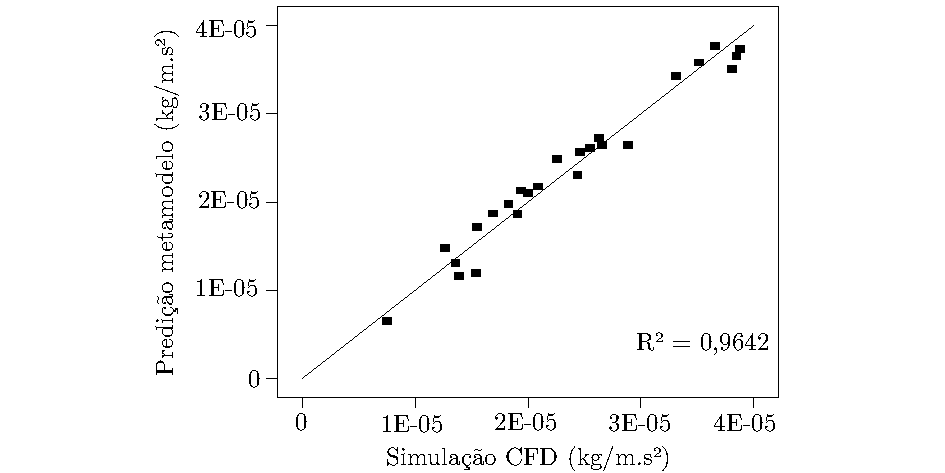
\includegraphics{Figuras/crossplotbehkhen.pdf}  
    \caption{Validação cruzada entre o modelo de Regressão e a simulação numérica CFD.}  
    \legend{Fonte: o autor.}
    \label{fig:validcruzada}  
\end{figure}

Por meio da análise da Figura \ref{fig:validcruzada}, é possível observar que o metamodelo está bem ajustado para as previsões de taxa de erosão, o que é esperado uma vez que os dados previstos foram os mesmos utilizados para geração do modelo. A presente análise constitui um procedimento preliminar, visando avaliar a adequação do modelo aos dados. É importante ressaltar que, em etapas subsequentes do estudo, serão realizados testes para verificar a capacidade de generalização do modelo para dados adicionais. Nesta etapa de avaliação do modelo, foi analisado o coeficiente de determinação R²=0.9642, o qual fornece um indicativo relevante sobre a capacidade preditiva do modelo. No entanto, é importante ressaltar que o valor de R² não oferece informações sobre possíveis vieses do modelo ou sua capacidade de generalização para dados não observados. Portanto, para mitigar esse aspecto, foi calculado o R² ajustado, uma métrica que considera a inclusão de variáveis adicionais no modelo e indica se elas contribuem significativamente para a capacidade de previsão. Além disso, foi obtido o R² previsto, uma medida de validação cruzada que avalia o desempenho do modelo ao remover sistematicamente cada observação da matriz de dados e estimar o valor correspondente com base na equação de regressão. Essa abordagem permite uma avaliação mais precisa da capacidade do modelo em lidar com dados não vistos anteriormente. A medida de Precisão adequada mede a relação sinal-ruído, que compara a faixa dos valores previstos nos pontos das observações com o erro médio de previsão, portanto razões maiores que 4 indicam  que o modelo é adequado. A Tabela \ref{tab:r2} demonstra o valores de R² e a Precisão adequada do modelo.


\begin{table}[!h]
\centering
\caption{Estatísticas de ajuste do modelo de regressão (Superfície de resposta).}
\begin{tabular*}{0.6\textwidth}{@{\extracolsep{\stretch{1}}}*{2}{c}@{}}
 \toprule
  Fonte&Valor\\
  \midrule

R²             & 0.9643  \\
R² Ajustado    & 0.9465  \\
R² Predito   & 0.9123  \\
Precisão adequada & 24.9635\\
Desvio padrão &2.08e-06\\
  \bottomrule   
\end{tabular*}
\label{tab:r2}

\legend {Fonte: o autor.}
\end{table*}
\end{table}

Os valores obtidos para  R², R² Predito e R² Ajustado, encontram-se muito próximos, considerando a pequena disparidade entre os valores em questão. Portanto a partir desta análise é possível inferir, através desta análise prévia, que não há razões para suspeitar que o modelo esteja viesado, o que será verificado de fato com a verificação da capacidade de generalização do modelo em dados ainda não vistos.

A medida de precisão adequada de 24.964 indica que o modelo possui uma proporção maior que 4 entre sinal e ruído. Isso sugere que a variação explicada pelos fatores independentes incluídos no modelo é significativamente maior do que a variação não explicada ou atribuível ao ruído aleatório.

Para serem utilizadas em previsões, o modelo deve atender a certos requisitos estatísticos \cite{montgomery}. Para tanto, foi aplicado o teste de normalidade (Figura \ref{fig:testeprobnormal}) para verificar se a distribuição dos resíduos aparenta ser normal.  Outra análise importante é a de que os resíduos devem possuir variância constante (homocedasticidade), ou seja, que o modelo de regressão obtido comete erros aleatórios e não prevê sistematicamente nenhum intervalo de valores de destino, a Figura \ref{fig:residuoshomoedasticidade} demonstra os resíduos do modelo.


\begin{figure}[H] 
    \centering  
    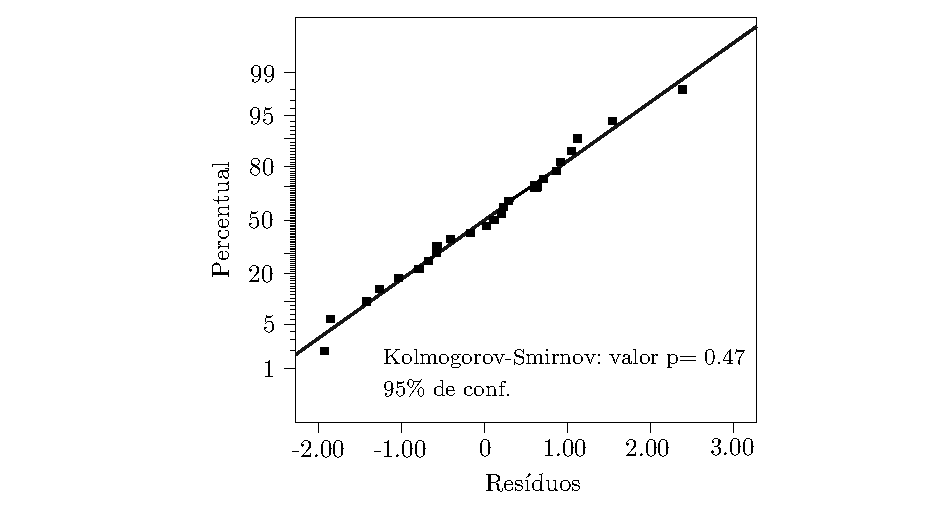
\includegraphics{Figuras/probnormal.pdf}  
    \caption{Gráfico de probabilidade normal.}  
    \legend{Fonte: o autor.}
    \label{fig:testeprobnormal}  
\end{figure}

\begin{figure}[H] 
    \centering  
    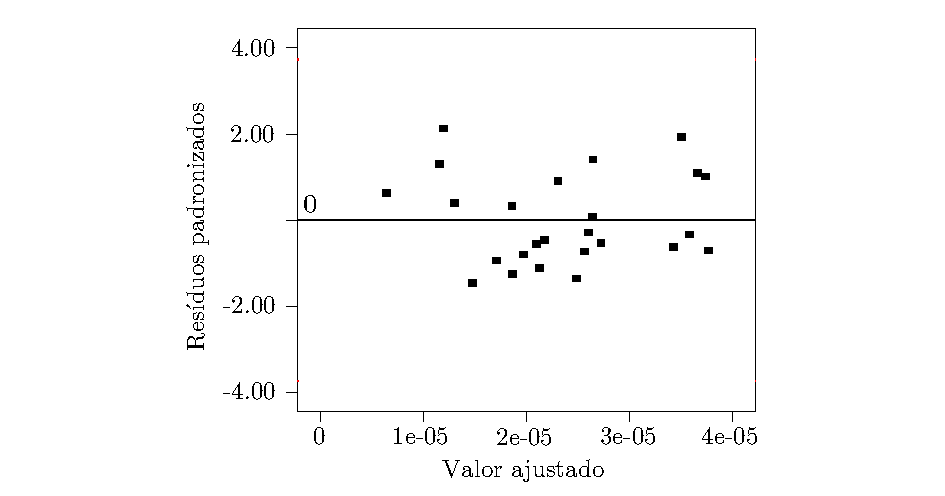
\includegraphics{Figuras/residuos.pdf}  
    \caption{Gráfico de resíduos padronizados.}  
    \legend{Fonte: o autor.}
    \label{fig:residuoshomoedasticidade}  
\end{figure}

A análise da Figura \ref{fig:testeprobnormal} permite determinar que os pontos se encontram próximos da linha reta, ou seja, a distribuição de erro é aproximadamente normal. Para validar esta hipótese, foi realizado o teste de normalidade de Kolmogorov-Smirnov. Para o ensaio de Box Behnken realizado, o valor p do teste Kolmogorov-Smirnov foi de 0.47, o que indica que os resíduos seguem uma distribuição normal. A Figura \ref{fig:residuoshomoedasticidade} não demonstra razão para suspeitar de qualquer violação das suposições de independência ou variância constante, ou seja, é possível verificar que os resíduos apresentam homocedasticidade.
Esse modelo de regressão gerado é composto por uma equação analítica, que contém termos lineares, quadráticos e de interação, que foram considerados como significativos através da análise de variância (Tabela \ref{tab:anovabox}). Na Tabela \ref{tab:box555} encontram-se os valores de erosão simulados para elaboração da superfície de resposta e os valores previstos pelo metamodelo de regressão, a partir das mesmas combinações dos parâmetros.

\begin{table}[H]
\caption{Matriz do planejamento Box Benhkhen para 4 variáveis de entrada.}
\begin{tabular*}{\textwidth}{@{\extracolsep{\stretch{1}}}*{7}{c}@{}}
 \toprule
   Simulação &VM	&VISC	&TAM	&VEL&Erosão OKA&Erosão Modelo	\\
  \midrule

1  & 0.13 & 15 & 0.55  & 9.50  & 1,92E-05 & 1,86E-05 \\
2  & 0.27 & 15& 0.55  & 9.50   & 3,88E-05 & 3,73E-05 \\
3  & 0.13 & 35& 0.55  & 9.50   & 1,28E-05 & 1,47E-05 \\
4  & 0.27 & 35 & 0.55  & 9.50  & 2,47E-05 & 2,57E-05 \\
5  & 0.20  & 25  & 0.24 & 8.87  & 1,36E-05 & 1,30E-05 \\
6  & 0.20  & 25  & 0.86 & 8.87  & 2,44E-05 & 2,31E-05 \\
7  & 0.20  & 25  & 0.24 & 10.13 & 1,70E-05 & 1,87E-05 \\
8  & 0.20  & 25  & 0.86 & 10.13 & 3,66E-05  & 3,76E-05 \\
9  & 0.13 & 25  & 0.55  & 8.87  & 1,38E-05 & 1,16E-05 \\
10 & 0.27 & 25  & 0.55  & 8.87  & 2,66E-05 & 2,64E-05 \\
11 & 0.13 & 25  & 0.55  & 10.13 & 2,09E-05 & 2,17E-05 \\
12 & 0.27 & 25  & 0.55  & 10.13 & 3,85E-05 & 3,66E-05 \\
13 & 0.20  & 15 & 0.24 & 9.50   & 1,83E-05 & 1,97E-05 \\
14 & 0.20  & 35 & 0.24 & 9.50   & 1,54E-05 & 1,20E-05 \\
15 & 0.20  & 15 & 0.86 & 9.50   & 3,31E-05 & 3,42E-05 \\
16 & 0.20  & 35 & 0.86 & 9.50   & 2,88E-05 & 2,65E-05 \\
17 & 0.13 & 25 & 0.24& 9.50  & 7,55E-06 & 6,46E-06 \\
18 & 0.27 & 25  & 0.24 & 9.50   & 1,95E-05 & 2,13E-05 \\
19 & 0.13 & 25  & 0.86 & 9.50   & 2,00E-05 & 2,10E-05 \\
20 & 0.27 & 25  & 0.86 & 9.50   & 3,51E-05 & 3,58E-05 \\
21 & 0.20  & 15 & 0.55  & 8.87  & 2,26E-05 & 2,49E-05 \\
22 & 0.20  & 35 & 0.55  & 8.87   & 1,56E-05 & 1,71E-05 \\
23 & 0.20  & 15 & 0.55  & 10.13 & 3,80E-05 & 3,50E-05 \\
24 & 0.20  & 35 & 0.55  & 10.13 & 2,63E-05 & 2,72E-05 \\
25 & 0.20  & 25  & 0.55  & 9.5    & 2,56E-05 & 2,61E-05\\

\bottomrule 
\end{tabular*}
\label{tab:box555}
\subcaption{VM: Vazão massica(kg/s); VISC: Viscosidade do fluido de perfuração(cP); TAM: Tamanho(mm); VEL: Velocidade de escoamento(m/s).}
\legend {Fonte: o autor.}
\end{table}


Após a validação estatística do modelo de Box Behnkhen, foram gerados as figuras com os termos lineares, quadráticos e de interação que compõe o modelo. Estes gráficos visam demonstrar como os termos influenciam na resposta do modelo. A Figura \ref{fig:efeitosbox1} 
apresenta o Gráfico de efeitos dos termos lineares que compõe o modelo. 


\begin{figure}[H] 
    \centering  
    \includegraphics{Figuras/efeitosdeinteracao - Cópia.pdf}  
    \caption{Gráfico de efeitos para o desgaste erosivo de Oka.}  
    \legend{Fonte: o autor.}
    \label{fig:efeitosbox1}  
\end{figure}

É possível observar que a Vazão mássica, Tamanho e Velocidade apresentam efeitos positivos no desgaste erosivo, ou seja, o aumento desses atributos ocasionam maiores desgates dentro das respectivas faixas de variação. O atributo Velocidade causa um aumento linear na resposta de erosão, enquanto que os atributos de Vazão mássica e Tamanho não apresentam relação linear com a variação do nível do atributo. 

Avaliar efeitos de interações é um dos principais objetivos dos planejamentos estatísticos. Se uma interação entre diferentes atributos for significativa, indica que a resposta de um fator depende da presença ou ausência do outro para a modelagem. Para estes casos, é pertinente o estudo do comportamento de um fator em relação a cada nível de outro fator. Em muitos casos, como o analisado na Tabela \ref{tab:anovabox}, somente alguns termos de interações contribuem efetivamente para a Soma de Quadrados da Interação e com significância adequadas para constituir o metamodelo de regressão.  As interações entre os atributos "Vazão mássica" e Viscosidade e "Tamanho e Velocidade", consideradas como significativas para o modelo, através da Análise de variância da Tabela \ref{tab:anovabox} se encontram dispostas na Figura \ref{fig:efeitosdeint}.

\begin{figure}[H] 
    \centering  
    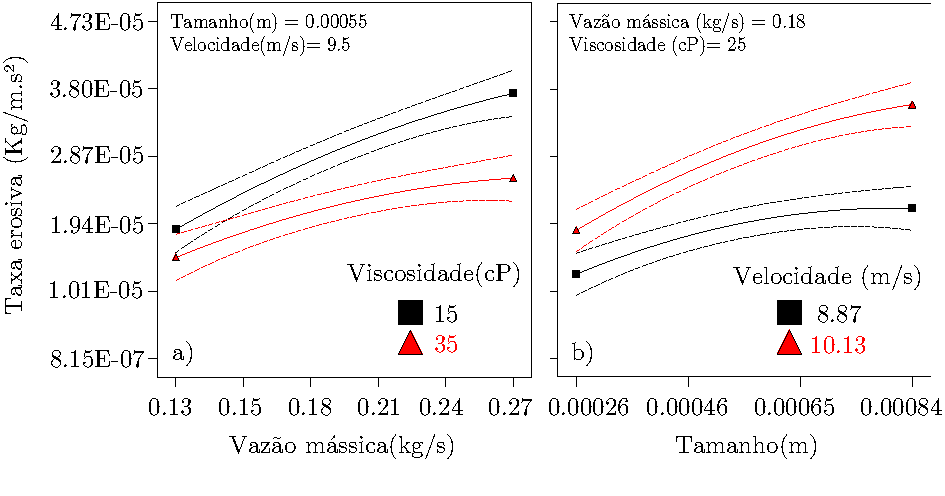
\includegraphics[width=0.95\textwidth]{Figuras/efeitosdeinteracao.pdf}  
    \caption{Efeitos de interação dos termos significativos do modelo de Box Behnken.}  
    \legend{Fonte: o autor.}
    \label{fig:efeitosdeint}  
\end{figure}



Através da análise da Figura \ref{fig:efeitosdeint}(a), é possível observar a interação entre "Vazão mássica e Viscosidade", o aumento da "Vazão mássica" propicia um desgaste erosivo maior em um nível inferior de "Viscosidade", e em "Viscosidade" mais alta embora haja um aumento da taxa erosiva, a magnitude de desgaste não é tão elevado quanto em menor "Viscosidade". Na Figura \ref{fig:efeitosdeint}(b) através da interação entre "Velocidade e Tamanho", é possível observar que numa condição de "Velocidade" maior e concomitante aumento de "Tamanho", dentro da faixa estudada, a taxa erosiva é mais elevada. Enquanto em "Velocidade" mais baixa, embora haja um aumento da taxa erosiva, a magnitude de desgaste não é tão elevado quanto em maior "Velocidade". A Figura \ref{fig:respostaveltam2o}, demonstra os gráficos de Superfície de resposta e contorno decorrente da interação dos atributos de "Viscosidade e Vazão mássica". Estes gráficos fornecem uma clara inspeção visual das interações entre os atributos e a magnitude na função-objetivo de desgaste erosivo.

\begin{figure}[H] 
    \centering  
    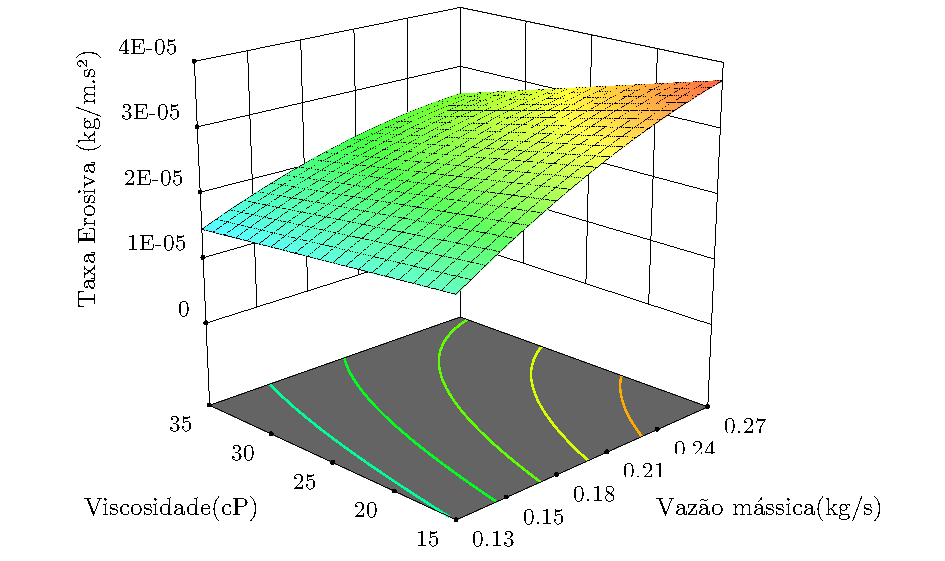
\includegraphics[width=0.88\textwidth]{Figuras/superficie2.pdf}  
    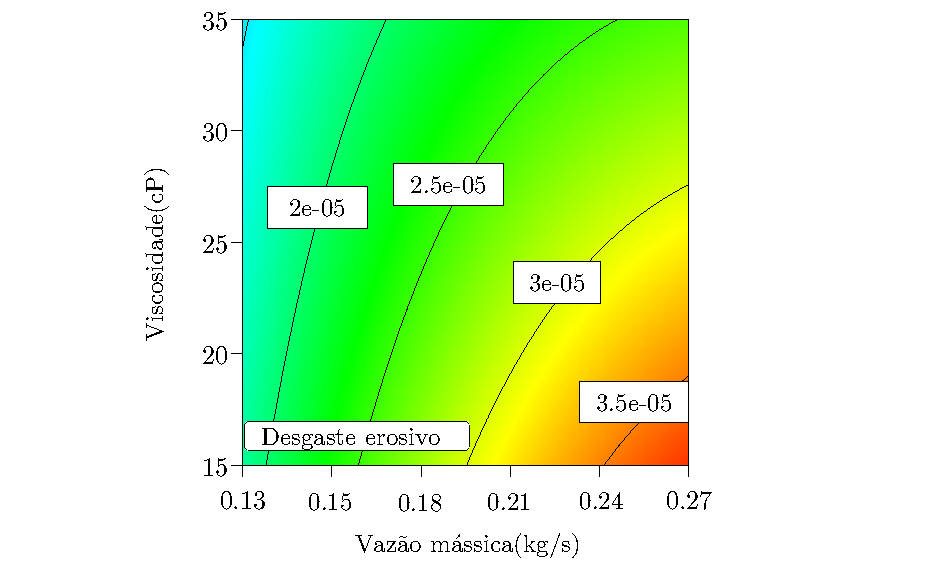
\includegraphics[width=0.88\textwidth]{Figuras/contornomassica.pdf}  
    \caption{Superfície de resposta e gráfico de contorno do efeito de Velocidade e Tamanho na resposta de taxa erosiva.}  
    \legend{Fonte: o autor.}
    \label{fig:respostaveltam2o}  
\end{figure}

Na análise da Figura \ref{fig:respostaveltam2o}, é evideciada a interação entre os termos de "Viscosidade do fluido de perfuração e Vazão mássica". Observa-se que a "Viscosidade" exerce uma influência direta na resposta da taxa erosiva. Para valores menores de "Viscosidade", é observada uma maior magnitude da taxa erosiva. Isso ocorre porque, nessas condições, as partículas sólidas têm maior tendência a se depositar na superfície do material, resultando em colisões mais frequentes nas paredes do material. Do contrário, uma maior "Viscosidade de fluido" causa uma maior tendência das partículas seguirem as linhas de corrente, o que reduz a frequência de impacto e, consequentemente, a taxa erosiva \cite{tsai}, \cite{yabuki}. A maior concentração de partículas presentes no fluxo, ou seja, aumento de "Vazão mássica" resulta em maior propensão ao desgaste, haja vista que a Erosão aumenta com a quantidade de partículas incidindo sobre a superfície do material alvo \cite{gandhi}. Assim, conforme o modelo, o aumento concomitante da "Viscosidade e Vazão mássica", provém o incremento da taxa erosiva para as faixas de variação estudadas. A Figura \ref{fig:respostaveltama}, demonstra os gráficos de Superfície de resposta e contorno decorrente da interação dos atributos de "Velocidade e Tamanho do cascalho".

\begin{figure}[H] 
    \centering  
    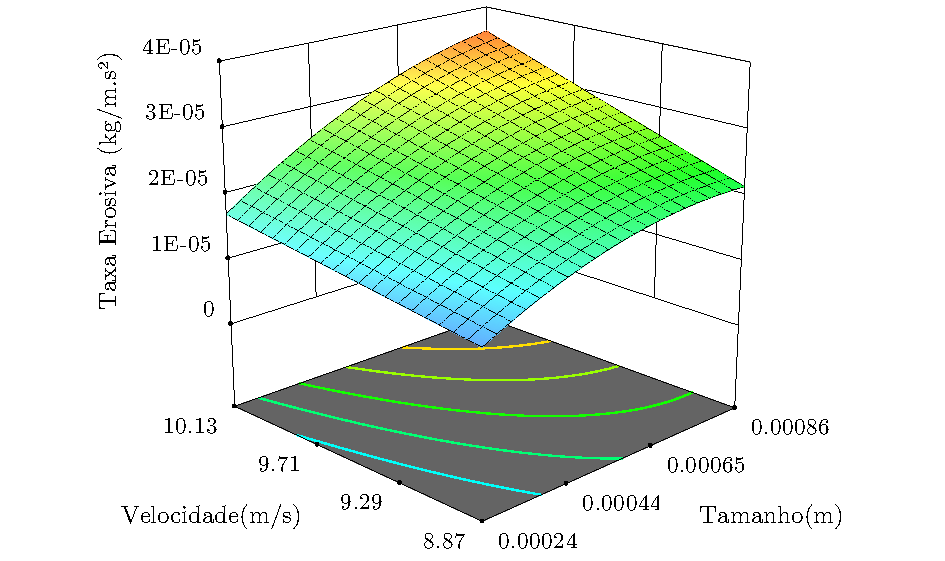
\includegraphics[width=0.84\textwidth]{Figuras/superficie.pdf}  
    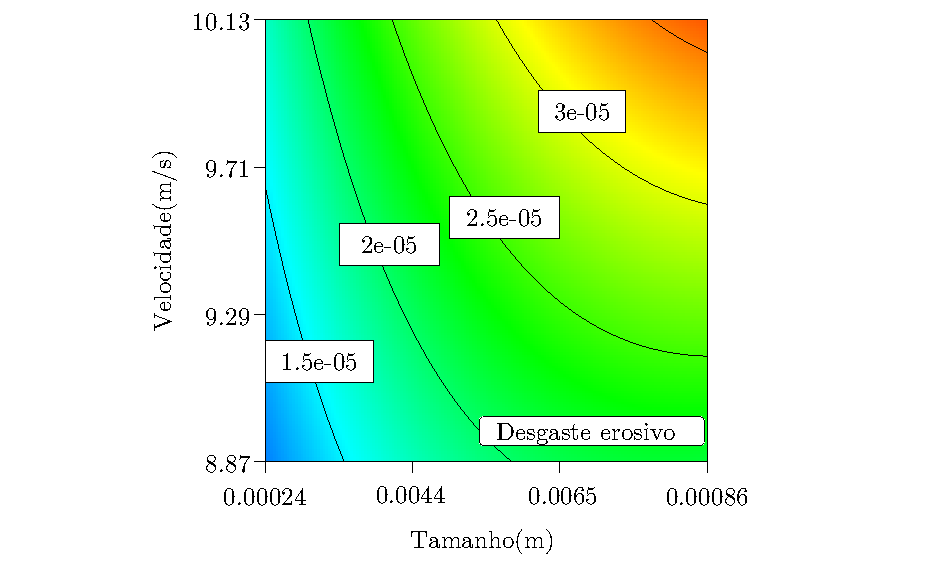
\includegraphics[width=0.84\textwidth]{Figuras/contorno2.pdf} 
    \caption{Superfície de resposta do efeito de Velocidade e Tamanho na resposta de taxa erosiva.}  
    \legend{Fonte: o autor.}
    \label{fig:respostaveltama}  
\end{figure}

Através da Figura \ref{fig:respostaveltama} é possível observar que partículas maiores resultam no aumento da taxa de erosão. Isto é explicado pois, além da maior energia de impacto, o tamanho da superfície de contato entre a partícula e a superfície tende a ser mais abrangente, levando a um maior desgaste no material \cite{lieb}, \cite{clark}. De mesmo modo, é possível verificar que em maiores Velocidades ocorre o aumento da taxa erosiva, em função da maior energia cinética de impacto \cite{lind}, \cite{finnie2}. De acordo com o metamodelo matemático, foi observada que o aumento concomitante dos valores dos atributos "Vazão mássica" e "Velocidade" resulta em cenários com maior desgaste erosivo, dentro das faixas de variação consideradas no estudo. Isso indica que os parâmetros influenciam de forma conjunta na resposta do modelo, e o aumento de seus valores contribui para um aumento no desgaste erosivo.

\section{Análise de risco através da Árvore de derivação}

Neste item, são obtidas e comparadas as curvas de Árvore de derivação por simulação numérica CFD e o modelo de regressão obtido pelo metamodelo de Superfície de resposta. O método da Árvore de derivação resultou em 81 cenários de simulação numérica, através da combinação de 3 níveis para as 4 variáveis definidas como críticas para o desgaste erosivo na etapa de triagem. Após simulação fludidinâmica dos cenários determinados, os dados foram tratados estatisticamente para obtenção da curva de risco de falha por Desgaste Erosivo (Figura \ref{fig:ad}).


\begin{figure}[H] 
    \centering  
    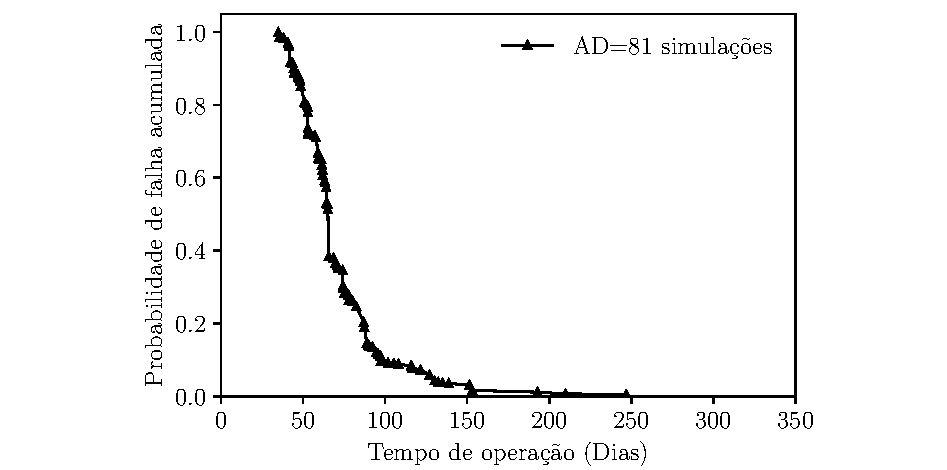
\includegraphics{Figuras/AD.pdf}  
    \caption{Árvore de derivação para 4 atributos com 3 níveis.}  
    \legend{Fonte: o autor.}
    \label{fig:ad}  
\end{figure}

Através da análise da curva de risco, é possível observar que os valores correspondentes aos percentis desse processo são respectivamente, P10 = 97.40 dias, P50 = 64.91 dias e P90 = 44.21 dias. As Figura \ref{fig:scattermodelo} e \ref{fig:compmetaarvore}, exibem os gráficos de validação cruzada e os valores comparativos entre os valores obtidos pelo metamodelo de regressão e as 81 simulações fluidodinâmicas CFD que compuseram a Árvore de derivação.

\begin{figure}[H] 
    \centering  
    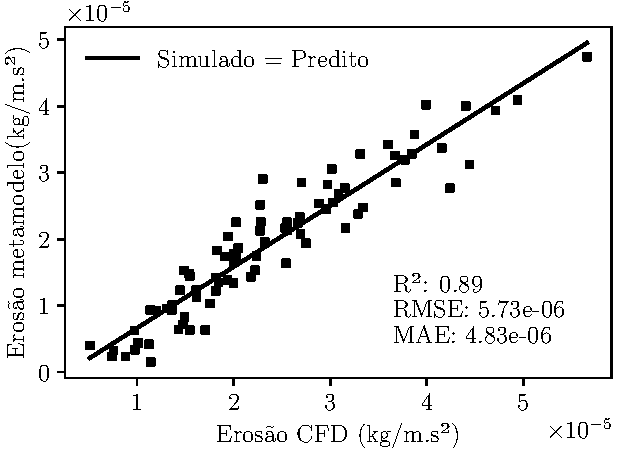
\includegraphics{Figuras/scatterModelo2.pdf}  
    \caption{Validação cruzada entre o metamodelo de Regressão e a simulação numérica CFD.}  
    \legend{Fonte: o autor.}
    \label{fig:scattermodelo}  
\end{figure}
\begin{figure}[H] 
    \centering  
    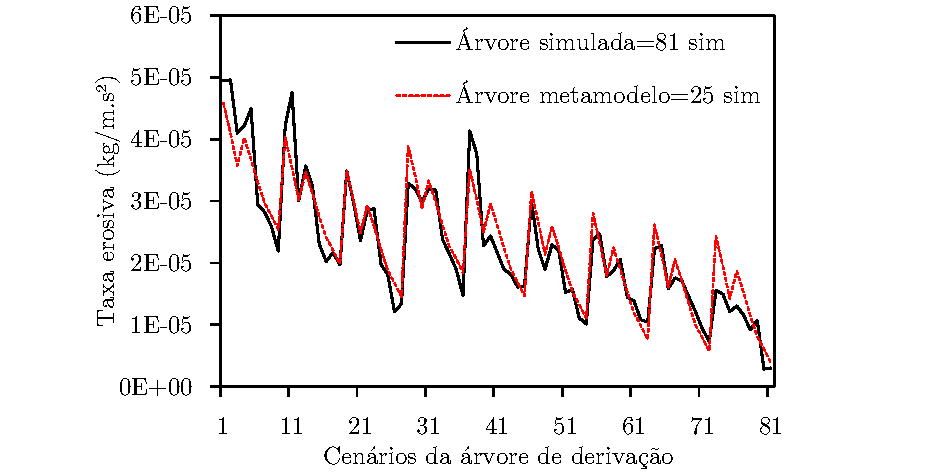
\includegraphics{Figuras/compmetaarvore.pdf}  
    \caption{Comparativo (Erosão CFD e Erosão pelo metamodelo de regressão.}  
    \legend{Fonte: o autor.}
    \label{fig:compmetaarvore}  
\end{figure}


Os resultados obtidos com o metamodelo de regressão demonstram uma capacidade satisfatória de prever os cenários da Árvore de derivação, como evidenciado pelas métricas R², RMSE e MAE. Isso indica que o modelo possui capacidade de realizar previsões em dados que não foram utilizados para a constituição do modelo. A Figura \ref{fig:compmetaarvore} ilustra como o modelo se ajustou adequadamente às variações das respostas dos cenários simulados pela Árvore de derivação. Além disso, a Figura \ref{fig:AdeAD} apresenta a comparação entre a curva de risco de falha por Erosão obtida por Simulações fluidodinâmicas computacionais para o método da Árvore de derivação e a curva de Árvore de derivação prevista pelo metamodelo de regressão.

\begin{figure}[H] 
    \centering  
    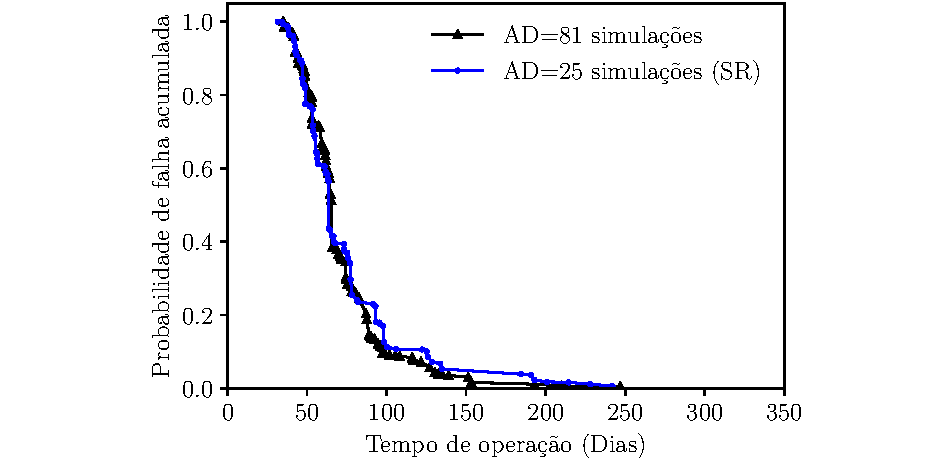
\includegraphics{Figuras/probacADeSR.pdf}  
    \caption{Curvas de risco por Árvore de derivação (CFD e Metamodelo).}  
    \legend{Fonte: o autor.}
    \label{fig:AdeAD}  
\end{figure}


Ao analisar o gráfico, podemos constatar que a curva de risco gerada pelo modelo de regressão se ajustou de forma satisfatória e apresentou uma proximidade significativa em relação à curva de referência, a qual é composta por todos os pontos simulados por CFD, assim como nos resultados de trabalhos anteriores para Análise de risco para estudos econômicos de projetos petrolíferos \cite{loschiavo},\cite{steagall}, \cite{santoss2}, \cite{yeten}, \cite{risso1}, \cite{slotte}  . Isso indica que o metamodelo é capaz de fornecer uma estimativa adequada da curva de risco. Para a curva de Árvore de derivação obtida pelo metamodelo foram necessárias 25 simulações fluidodinâmicas, o que representa uma redução de aproximadamente 69\% do número de simulações requeridas para obtenção da curva de risco, resultando em um esforço computacional menor. A Tabela \ref{tab:percentisadsr} apresenta a comparação dos percentis (P10, P50 e P90) entre a curva de risco obtida pela simulação numérica e pela superfície de resposta.

\begin{table}[h]
\caption{Comparação entre os percentis das curvas de risco de falha por simulação CFD e Metamodelo (SR).}
\begin{tabular*}{\textwidth}{@{\extracolsep{\stretch{1}}}*{4}{c}@{}}
 
  \toprule
    Percentil& Árvore de derivação (CFD) & Árvore de derivação (SR)  & Variação  \\
  (\%)& falha (dias) & falha (dias) &(\%)   \\
  \midrule
   P10&	97.40 	&100.70 &3.27\%\\
  P50 &	 64.91	&63.64& -1.95\%\\
 P90 &	44.21	&45.16 &2.14\%\\

  \bottomrule   
\end{tabular*}
\label{tab:percentisadsr}
\legend {Fonte: o autor.}
\end{table*}
\end{table}

A curva obtidas pelo modelo de regressão aplicada à árvore de derivação demonstrou bons resultados sendo o maior diferencial de percentis de 3.27\% para o P10, -1.95\% para o P50 e 2.14\% para o P90, comparado com a curva de Árvore de derivação simulada de referência. O próximo capítulo demonstra as curvas de risco pelo método de Monte Carlo obtidas pelo metamodelo de regressão.

\section{Análise de risco através de Monte Carlo}

     Nesta etapa, foi realizada a geração das curvas de risco segundo os sorteios de Monte Carlo e comparadas com a Árvore de derivação gerada por simulações fluidodinâmicas. Para a composição das curvas de risco por Monte Carlo foram obtidos diferentes cenários variando entre 100 e 80000 valores, seguindo a distribuição de probabilidade das variáveis aleatórias. Os resultados de erosão de cada cenário realizado pelos sorteios foram obtidos pelo metamodelo de regressão. Com as amostras obtidas por Monte Carlo, é possível a obtenção da média e desvio padrão da erosão para cada distribuição amostral, e deste modo realizar o cálculo de Cov (coeficiente de variação) para cada conjunto (Figura \ref{fig:mc}).  


\begin{figure}[H] 
    \centering  
    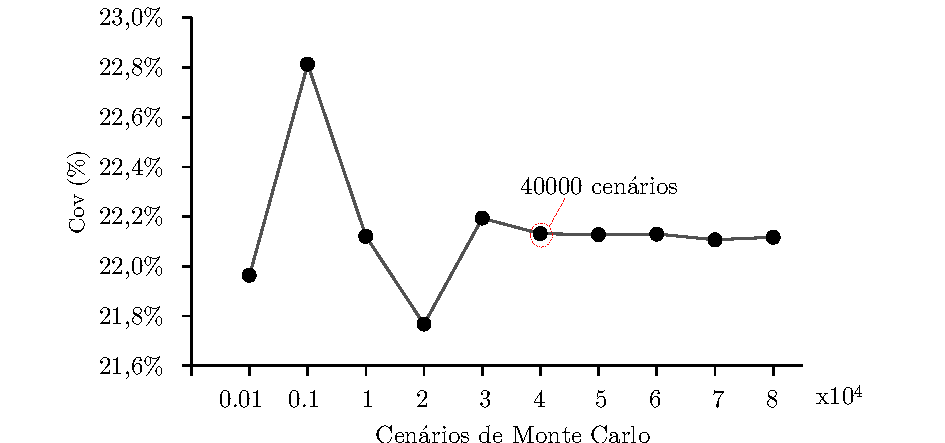
\includegraphics[width=0.83\textwidth]{Figuras/mcsorteios.pdf}  
    \caption{Coeficiente de variação para os cenários de Monte Carlo.}  
    \legend{Fonte: o autor.}
    \label{fig:mc}  
\end{figure}

 É possível verificar através da análise do Cov, que a partir de 40000 amostras, a erosão do modelo de Oka passa a produzir uma estimativa consistente da função de distribuição de probabilidade. A Figura \ref{fig:mca} demonstra as distribuições de probabilidade de diferentes quantidades amostrais obtidas por Monte Carlo.

\begin{figure}[H] 
    \begin{minipage}[!]{0.50\linewidth}
    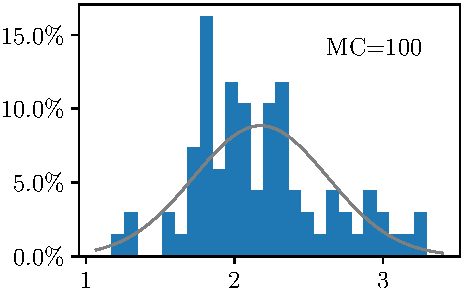
\includegraphics[\width=\linewidth]{Figuras/100.pdf}
    \end{minipage}
    \begin{minipage}[!]{0.50\linewidth}
    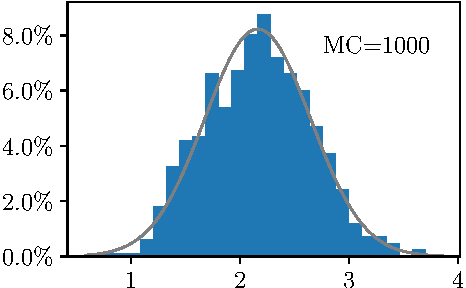
\includegraphics[\width=\linewidth]{Figuras/1000.pdf}
    \end{minipage}
    \begin{minipage}[!]{0.50\linewidth}
    \centering
    \includegraphics[\width=\linewidth]{marca}\\ {Erosão kg/m.s² (x10^{-5})}
    \end{minipage}
    \begin{minipage}[!]{0.50\linewidth}
    \centering
    \includegraphics[\width=\linewidth]{marca}\\ {Erosão kg/m.s² (x10^{-5})}
    \end{minipage}
   

    \begin{minipage}[!]{0.50\linewidth}
    \includegraphics[\width=\linewidth]{Figuras/40000.pdf}
    \end{minipage}
    \begin{minipage}[!]{0.50\linewidth}
    \includegraphics[\width=\linewidth]{Figuras/60000.pdf}
    \end{minipage}
    \begin{minipage}[!]{0.50\linewidth}
    \centering
    \includegraphics[\width=\linewidth]{marca}\\ {Erosão kg/m.s² (x10^{-5})}
    \end{minipage}
    \begin{minipage}[!]{0.50\linewidth}
    \centering
    \includegraphics[\width=\linewidth]{marca}\\ {Erosão kg/m.s² (x10^{-5})}
    \end{minipage}
    \caption{Distribuição da resposta de Erosão em diferentes cenários de Monte Carlo.}
    \legend{Fonte: o autor.}
    \label{fig:mca}
\end{figure}

Através das distribuições de probabilidade, é verificado que em 100 cenários de Monte carlo a curva de distribuição ainda não apresenta uma estimativa consistente da distribuição da resposta, conforme aumenta o número de cenários é possível constatar que a média e desvio-padrão se estabilizam e a curva apresenta distribuição estável e consistente. A Figura \ref{fig:mc222} demonstra as comparações das distribuições segundo as diferentes combinações de cenários de Monte Carlo, o que reforça o indicativo de estabilização a partir de 40.000 cenários de combinações das variáveis para geração da resposta. 


\begin{figure}[H] 
    \centering  
    \includegraphics{Figuras/boxplots.pdf}  
    \caption{Box plots da Distribuição da resposta de Erosão em diferentes cenários de Monte Carlo.}  
    \legend{Fonte: o autor.}
    \label{fig:mc222}  
\end{figure}

A partir das respostas obtidas foram plotadas curvas de risco geradas pelos diferentes cenários
de sorteios, para avaliar a influência na qualidade da curva de risco. A Figura \ref{fig:mc2} apresenta a curva de risco de falha por erosão, obtidas por Árvore de derivação (CFD) e as obtidas pelos cenários gerados por Monte Carlo.


\begin{figure}[H] 
    \centering  
    \includegraphics{Figuras/mc.pdf}  
    \caption{Curvas de risco Monte Carlo e Árvore de derivação.}  
    \legend{Fonte: o autor.}
    \label{fig:mc2}  
\end{figure}



Os sorteios gerados pelo método de Monte Carlo com as distribuições das variáveis contínuas, e com a aplicação da superfície de resposta, apresentaram curvas muito próximas da obtida pela Árvore de derivação gerada com 81 simulações fluidodinâmicas, especialmente as curvas com 40000 sorteios e 60000 sorteios. Como não houve grande variação entre os sorteios de 40000 e 60000 é aceitável determinar que 40000 cenários evidencia o número de sorteios ideal para reprodução da distribuição dos atributos para previsão do desgaste erosivo. A Tabela \ref{tab:percentisadmc} apresenta a comparação dos percentis (P10, P50 e P90) entre a curva de risco da Árvore de derivação, obtida pela simulação numérica e as curvas de Monte Carlo geradas pelo modelo de superfície de resposta.


\begin{table}[h]
\caption{Comparação entre os percentis das curvas de risco de falha por simulação CFD e Metamodelo (SR) para cenários de Monte Carlo.}
\begin{tabular*}{\textwidth}{@{\extracolsep{\stretch{1}}}*{5}{c}@{}}
 
  \toprule
    Percentil&  MC 1000 (SR) & MC 40000 (SR)& MC 60000 (SR)&MC 80000(SR)  \\
 (\%) &   Variação(\%) &Variação(\%)& Variação(\%)& Variação(\%)  \\
  \midrule
   P10	& 8.41\%&1,45\%&1.43\%&1.52\%\\
  P50 	& 0.47\%&0.62\%& 0.59\%&0.61\%\\
 P90 	& 16.03\%&1.99\%&2.08\%&2.11\%\\

  \bottomrule   
\end{tabular*}
\label{tab:percentisadmc}
\subcaption{Diferenças percentuais em módulo.}
\legend {Fonte: o autor.}

\end{table*}
\end{table}

A curva de risco obtida através da técnica de Monte Carlo com 1000 sorteios apresenta diferença de 16.03\% em relação ao percentil P90, 8.41\% em relação ao P10 e 0.47\% para P50 da curva gerada por Simulação computacional para Árvore de derivação. Porém, as curvas de risco geradas com 40000, 60000 e 80000 sorteios de Monte Carlo se encontram muito próximas entre si e em relação à curva de risco de Árvore de derivação de referência.  Deste modo, é possível verificar que as variações percentuais atingiram estabilização, não havendo grandes mudanças nas magnitudes dos percentis com o aumento de sorteios a partir de 40000 combinações de Monte Carlo, o que reitera as análises gráficas das Figuras \ref{fig:mc}, \ref{fig:mca} e \ref{fig:mc222}.

As diferenças percentuais entre os valores obtidos para os percentis da Árvore de derivação e Monte Carlo, ocorre pelas diferenciações que as técnicas apresentam quanto ao método de combinação dos atributos aleatórios para geração dos cenários de erosão. Neste sentido, o método de Monte Carlo apresenta maior confiabilidade do ponto de vista amostral, uma vez que as são obtidas quantidades amostrais sificientemente representativas para composição das simulações até que se alcance estabilidade numérica na resposta. Por outro lado, os cenários obtidos através do método de Árvore de derivação gerados a partir da discretização dos atributos, embora seja mais simples do ponto de vista amostral, obteve os resultados de desgaste erosivo diretamente a partir de simulações numéricas por CFD, não sendo necessário obrigatoriamente uma aplicação de um modelo de regressão para previsão dos dados de resposta.

Ademais, as obtenções dos desgastes erosivos de \citeonline{oka} para o método de Monte Carlo, foram obtidas pelo metamodelo de regressão, o que apresenta erros de aproximação inerentes aos métodos de regressão. Estes resultados demostram que a técnica de Monte Carlo e a técnica de Árvore de derivação apresentam resultados similares para obtenção de curva de risco de falha por erosão, uma vez que sejam utilizados metamodelos validados estatísticamente e sorteios amostrais suficientemente representativos das distribuições das variáveis aleatórias. Sendo métodos que podem ser aplicados concomitantemente para uma análise de risco mais rigorosa e com maior confiabilidade para a tomada de decisão referente à projetos do setor petrolífero.

  





\chapter{Conclusão}

Este trabalho realizou um estudo de análise de risco de falha por erosão para uma tubulação de 3 polegadas de diâmetro nominal utilizada em sistemas hidráulicos de perfuração de poços petrolíferos. 
Para obtenção e comparação dos cenários provenientes da combinação das variáveis aleatórias que influenciam no desgaste erosivo, foram aplicados os seguintes métodos de análise de risco: (1) método da árvore de derivação com simulações computacionais CFD, (2) o método da árvore de derivação com metamodelo de superfície de resposta e (3) método de Monte Carlo com metamodelo de superfície de resposta.

Com intuito de obter as previsões quantitativas do desgaste erosivo, foram realizadas simulações fluidodinâmicas computacionais que propiciaram a modelagem de escoamentos multifásicos complexos com fluido e cascalhos de perfuração, com objetivo de obter as regiões mais propensas ao impacto dos particulados em determinadas condições de fluxo. Através da modelagem do escoamento, foi possível identificar o local de maior desgaste erosivo na tubulação curva e quantificar esse desgaste. Essa análise possibilitou a estimativa do tempo de falha do material em condições operacionais específicas, abrangendo as diversas condições requeridas para o estudo.

Com objetivo de realizar a triagem dos atributos que mais influenciam no Desgaste erosivo para as faixas estudadas das variáveis aleatórias, o método de planejamento de Plackett-Burman forneceu respostas semelhantes em relação à análise de sensibilidade. A análise de sensibilidade demonstrou apenas o impacto que a variação de níveis dos atributos causaram no desgaste erosivo, ficando a critério do pesquisador a seleção da quantidade de atributos para aplicação da análise de risco. Por outro lado, o Planejamento de Plackett Burman, forneceu os efeitos dos atributos mais significativos no desgaste erosivo através de testes estatísticos, sendo em geral, mais confiável para seleção dos atributos críticos, além de apresentar um critério de corte de variáveis com base na significância estatística.

A etapa de análise de risco foi viabilizada através da utilização de um metamodelo de regressão obtido por meio do Planejamento Estatístico Box Behnken. O desempenho desse metamodelo foi avaliado comparando suas previsões com os resultados obtidos por Simulação fluidodinâmica. Os resultados revelaram que o metamodelo apresentou uma capacidade satisfatória de prever os cenários de Desgaste erosivo, quando comparado aos resultados da simulação. Essa conclusão é suportada pelas métricas de avaliação, como R2, RMSE e MAE, que indicam uma boa capacidade de generalização do modelo, permitindo fazer previsões para cenários que não foram utilizados durante a construção do metamodelo. Além disso, foi constatado que o metamodelo se ajustou adequadamente às variações das respostas dos 81 cenários simulados pela Árvore de Derivação pela comparação dos percentis P10, P50 e P90 com redução de 69\% no número de simulações fluidodinâmicas. 

No estudo de análise de risco utilizando a abordagem do Método de Monte Carlo (MC), foram gerados 301.100 cenários acumulados para verificação da estabilização da resposta. Através da análise de Cov foi constatado equilibrio de resposta em aproximadamente 40.000 iterações, o que se mostraria impraticável do ponto de vista computacional, caso realizadas as simulações numéricas por CFD. Portanto, a utilização do metamodelo para o método de Monte Carlo foi fundamental para a obtenção dos cenários de erosão e realização da análise de risco. Dessa forma, o metamodelo fundamentado na Superfície de Resposta desempenhou um papel satisfatório ao substituir o simulador fluidodinâmico na obtenção das curvas de risco relacionadas ao desgaste erosivo. Ao oferecer confiabilidade estatística e reduzir significativamente a carga computacional, essa abordagem se estabelece como uma ferramenta confiável para a previsão do fenômeno de desgaste erosivo para análise de risco de um projeto petrolífero.

As diferenças percentuais entre os valores obtidos para os percentis da Árvore de derivação e Monte Carlo ocorreu devido às diferentes abordagens utilizadas para combinar os atributos aleatórios na geração dos cenários de erosão. O método de Monte Carlo oferece maior confiabilidade amostral, por apresentar um grande número de amostras das variáveis aleatórias e exercer uma análise de estabilização da resposta. Por outro lado, a Árvore de derivação completa propicia a geração de cenários diretamente a partir de simulações numéricas por CFD, sem a necessidade de utilização de um modelo de regressão para previsão dos dados. Os resultados indicaram que Monte Carlo e Árvore de derivação apresentam respostas similares de curva de risco de falha por erosão, desde que sejam utilizados metamodelos validados estatisticamente e sorteios amostrais representativos das distribuições das variáveis aleatórias, o que contribui para a tomada de decisão de um projeto.
 
Dessa forma, por meio da aplicação e análise de uma metodologia de análise de risco, é viável determinar o tempo estimado até a falha dos materiais empregados na perfuração de poços, considerando o espectro de probabilidades de falha decorrente do desgaste erosivo ao qual a tubulação do sistema hidráulico está sujeita sob condições operacionais incertas. Essa análise fornece uma base sólida para a tomada de decisões relacionadas à manutenção e substituição das tubulações antes do rompimento. Com base no tempo de falha indicado pela curva de risco e considerando o projeto de perfuração específico, é possível considerar a utilização de materiais mais resistentes à erosão, como os Flanges Alvo ("Target Flanges"), que possuem um custo de aquisição mais elevado em comparação com as tubulações curvas convencionais. No entanto, esses materiais oferecem uma maior durabilidade, o que pode resultar em economia ao reduzir a necessidade de substituições frequentes. Ao optar pelos Flanges Alvo, é possível obter uma maior vida útil operacional, o que compensa os custos iniciais mais altos e contribui para uma gestão mais eficiente dos recursos e do orçamento relacionados à manutenção das tubulações.
 
\section{Sugestões de trabalhos futuros}

Como sugestão de trabalhos futuros, seguem as recomendações:

a) Estudar outros métodos de obtenção de metamodelos como, por exemplo, Aprendizado de máquinas e Planejamento de Composto Central;

b) Realizar análise econômica de um projeto, a partir da Análise de risco, para avaliar a vantagem da utilização de material com maior resistência ao desgaste erosivo (\textlit{Target Flanges}) em substituição à curva de Aço-carbono;

c) Avaliar desgaste erosivo através de outros modelos, tais como: Finnie, DNV, Tulsa;

d) Realizar estudo de Simulação Fluidodinâmica transiente para obtenção do desgaste erosivo para realização da Análise de risco.

e) Obtenção de dados reais de perfuração em campo para caracterização amostral das variáveis aleatórias que influenciam no desgaste erosivo e realizar testes de aderência amostrais. 

f) Avaliar a correlação e interdependência entre as variáveis aleatórias.

g) Validação experimental das Simulações Numéricas e do metamodelo de Superfície de resposta para previsão do desgaste erosivo.


% ----------------------------------------------------------
% Referências bibliográficas
% ----------------------------------------------------------
\bibliography{abntex2-modelo-references}

\end{document}
